\newcommand*{\BeamerSuffix}{-pres}
\newcommand*{\TransSuffix}{-slides}
% \documentclass{beamerswitch}
\documentclass[handout]{beamer}
\setbeamertemplate{navigation symbols}{}

\usepackage{movie15}
\usepackage{amssymb,amsmath}
\usepackage{hyperref}
\usepackage{natbib} 
\usepackage{pgf} 
\usepackage{mathtools}
\usepackage{tikz}
\usepackage{bbm}

\usetheme{Madrid}	% clean, nice.  7/12 page numbers




%\newtheorem{example}{Example}

\newcommand{\expect}{\mathbb{E}}
\newcommand{\variance}{\mathrm{Var}}
\DeclareMathOperator*{\Var}{Var}
\newcommand{\covariance}{\mathrm{Cov}}
\DeclareMathOperator*{\Cov}{Cov}
\newcommand{\prob}{\mathrm{Pr}}
\newcommand{\zeroVec}{\mathbf{0}}
\newcommand{\zeroMat}{\mathbf{0}}
\newcommand{\onesVec}{\mathbf{1}}
\newcommand{\ident}{\mathbf{I}}
\newcommand{\deriv}{\mathrm{d}}
\newcommand{\transpose}{\top}
\newcommand{\costDeriv}[1]{\overline{#1}}
\newcommand{\lossDeriv}{\costDeriv}
\newcommand{\normal}{\mathcal{N}}
\newcommand{\data}{\mathcal{D}}

\newcommand{\dataIdx}{i}
\newcommand{\featIdx}{j}
\newcommand{\dimIdx}{\featIdx}
\newcommand{\paramIdx}{\dimIdx}
\newcommand{\hidIdx}{i}
\newcommand{\classIdx}{k}
\newcommand{\outputIdx}{k}
\newcommand{\classIdxTwo}{\ell}
\newcommand{\featIdxTwo}{j^\prime}
\newcommand{\nfeat}{D}
\newcommand{\ndim}{\nfeat}
\newcommand{\ndata}{N}
\newcommand{\numClasses}{K}
\newcommand{\nout}{\numClasses}
\newcommand{\layerIdx}{\ell}
\newcommand{\numLayers}{L}
\newcommand{\nhid}{M}
\newcommand{\timeIdx}{t}
\newcommand{\ntime}{T}
\newcommand{\contextLen}{K}


\newcommand{\inputIJ}[2]{x^{(#1)}_{#2}}
\newcommand{\inputI}[1]{{\bf x}^{(#1)}}
\newcommand{\inputJ}[1]{x_{#1}}
\newcommand{\inputVec}{{\bf x}}
\newcommand{\inputVecT}[1]{\inputVec^{(#1)}}
\newcommand{\inputVecI}[1]{\inputVec^{(#1)}}
\newcommand{\inputUni}{x}
\newcommand{\inputUniI}[1]{x^{(#1)}}
\newcommand{\inputUniT}[1]{x^{(#1)}}
\newcommand{\inputMatrix}{\mathbf{X}}
\newcommand{\inputMatrixT}[1]{\inputMatrix^{(#1)}}
\newcommand{\targetI}[1]{t^{(#1)}}
\newcommand{\target}{t}
\newcommand{\targetK}[1]{\target_{#1}}
\newcommand{\targets}{\mathbf{t}}
\newcommand{\prediction}{y}
\newcommand{\predictionI}[1]{y^{(#1)}}
\newcommand{\predictionK}[1]{y_{#1}}
\newcommand{\predictionT}[1]{y^{(#1)}}
\newcommand{\predictions}{\mathbf{y}}
\newcommand{\predictionMatrix}{\mathbf{Y}}
\newcommand{\predictionMatrixT}[1]{\predictionMatrix^{(#1)}}
\newcommand{\intermediate}{z}
\newcommand{\intermediateI}[1]{\intermediate^{(#1)}}
\newcommand{\intermediateT}[1]{\intermediate^{(#1)}}
\newcommand{\intermediateK}[1]{\intermediate_{#1}}
\newcommand{\intermediates}{\mathbf{z}}
\newcommand{\intermediateMatrix}{\mathbf{Z}}
\newcommand{\intermediateMatrixT}[1]{\intermediateMatrix^{(#1)}}
\newcommand{\outIntermediate}{r}
\newcommand{\outIntermediateT}[1]{r^{(#1)}}
\newcommand{\outIntermediateK}[1]{\outIntermediate_{#1}}
\newcommand{\outIntermediates}{\mathbf{r}}
\newcommand{\outIntermediateMat}{\mathbf{R}}
\newcommand{\outIntermediateMatrix}{\mathbf{R}}
\newcommand{\outIntermediateMatrixT}[1]{\outIntermediateMatrix^{(#1)}}
\newcommand{\hiddenI}[1]{h_{#1}}
\newcommand{\hiddenT}[1]{h^{(#1)}}
\newcommand{\hiddenIT}[2]{h_{#1}^{(#2)}}
\newcommand{\hiddenLI}[2]{h_{#2}^{(#1)}}
\newcommand{\hiddens}{\mathbf{h}}
\newcommand{\hiddensL}[1]{\hiddens^{(#1)}}
\newcommand{\hiddensT}[1]{\hiddens^{(#1)}}
\newcommand{\hiddenMatrix}{\mathbf{H}}
\newcommand{\hiddenMat}{\hiddenMatrix}
\newcommand{\hiddenMatrixT}[1]{\hiddenMatrix^{(#1)}}
\newcommand{\hiddenMatL}[1]{\hiddenMat^{(#1)}}
\newcommand{\weights}{{\bf w}}
\newcommand{\weightsL}[1]{\weights^{(#1)}}
\newcommand{\weightJ}[1]{w_{#1}}
\newcommand{\weightLIJ}[3]{w^{(#1)}_{#2 #3}}
\newcommand{\weightLKI}[3]{w^{(#1)}_{#2 #3}}
\newcommand{\weightLJ}[2]{w^{(#1)}_{#2}}
\newcommand{\weightKJ}[2]{w_{#1 #2}}
\newcommand{\weightIJ}{\weightKJ}
\newcommand{\weightUni}{w}
\newcommand{\weightMat}{\mathbf{W}}
\newcommand{\weightMatL}[1]{\weightMat^{(#1)}}
\newcommand{\bias}{b}
\newcommand{\biasLI}[2]{\bias^{(#1)}_{#2}}
\newcommand{\biasLK}{\biasLI}
\newcommand{\biasL}[1]{\bias^{(#1)}}
\newcommand{\biasK}[1]{\bias_{#1}}
\newcommand{\biasJ}[1]{\bias_{#1}}
\newcommand{\biases}{\mathbf{b}}
\newcommand{\biasesL}[1]{\biases^{(#1)}}
\newcommand{\threshold}{r}
\newcommand{\featureJ}[1]{\psi_{#1}}
\newcommand{\featureVec}{{\boldsymbol \psi}}
\newcommand{\loss}{\mathcal{L}}
\newcommand{\lossI}[1]{\loss^{(#1)}}
\newcommand{\zeroOneLoss}{\loss_{\rm 0-1}}
\newcommand{\squaredErrorLoss}{\loss_{\rm SE}}
\newcommand{\crossEntropyLoss}{\loss_{\rm CE}}
\newcommand{\logisticCrossEntropyLoss}{\loss_{\rm LCE}}
\newcommand{\softmaxCrossEntropyLoss}{\loss_{\rm SCE}}
\newcommand{\hingeLoss}{\loss_{\rm H}}
\newcommand{\cost}{\mathcal{J}}
\newcommand{\regularizer}{\mathcal{R}}
\newcommand{\lrate}{\alpha}
\newcommand{\learningRate}{\lrate}
\newcommand{\featureMap}{{\boldsymbol \psi}}
\newcommand{\featureMapJ}[1]{\psi_{#1}}
\newcommand{\sigmoid}{\sigma}
\newcommand{\logistic}{\sigmoid}
\newcommand{\activationFunction}{\phi}
\newcommand{\activationFunctionL}[1]{\activationFunction^{(#1)}}
\newcommand{\activationFunctionTwo}{\psi}
\newcommand{\parityFunction}{f_{\rm par}}
\newcommand{\function}{f}
\newcommand{\functionL}[1]{\function^{(#1)}}
\newcommand{\indicatorOf}[1]{\mathbbm{1}_{#1}}
\newcommand{\softmax}{\mathrm{softmax}}
\newcommand{\weightCost}{\lambda}
\newcommand{\genCost}{\mathcal{C}}
\newcommand{\momentumVec}{\mathbf{p}}
\newcommand{\momentumJ}[1]{p_{#1}}
\newcommand{\momentumParam}{\mu}
\newcommand{\genParams}{{\boldsymbol \theta}}
\newcommand{\genParamJ}[1]{\theta_{#1}}
\newcommand{\pData}{p_{\mathcal{D}}}
\newcommand{\bestPrediction}{\prediction_\star}

\newcommand{\obs}{\mathbf{x}}
\newcommand{\obsJ}[1]{x_{#1}}
\newcommand{\obsI}[1]{\obs^{(#1)}}
\newcommand{\pfn}{\mathcal{Z}}
\newcommand{\happiness}{H}
\newcommand{\latents}{\mathbf{z}}

\newcommand{\state}{\mathbf{s}}
\newcommand{\stateT}[1]{\state_{#1}}
\newcommand{\act}{\mathbf{a}}
\newcommand{\actT}[1]{\act_{#1}}
\newcommand{\reward}{r}
\newcommand{\policy}{\pi}
\newcommand{\policyParams}{\boldsymbol{\theta}}
\newcommand{\policyTh}{{\policy_{\policyParams}}}
\newcommand{\MDP}{\mathcal{M}}
\newcommand{\rollout}{\tau}
\newcommand{\expectedReturn}{R}

\newcommand{\discReturn}{G}
\newcommand{\discFactor}{\gamma}
\newcommand{\valueFunc}{V}
\newcommand{\valueFuncPi}{\valueFunc^{\policy}}
\newcommand{\valueFuncPiTh}{\valueFunc^{\policyTh}}
\newcommand{\qFunc}{Q}
\newcommand{\qFuncPi}{\qFunc^{\policy}}
\newcommand{\optPolicy}{\policy^*}
\newcommand{\optQ}{\qFunc^*}

\newcommand{\subspace}{\mathcal{S}}
\newcommand{\projectedInput}{\tilde{\inputVec}}
\newcommand{\projectedInputI}[1]{\projectedInput^{(#1)}}
\newcommand{\codeVec}{\mathbf{z}}
\newcommand{\codeVecI}[1]{\codeVec^{(#1)}}
\newcommand{\dataMean}{\boldsymbol{\mu}}
\newcommand{\dataCov}{\boldsymbol{\Sigma}}
\newcommand{\pcaVec}{\mathbf{u}}

\newcommand{\featureMatrix}{{\boldsymbol \Psi}}
\newcommand{\smootherMatrix}{{\boldsymbol \Omega}}
\newcommand{\smootherMatrixEntry}{\Omega}
\newcommand{\hypothesis}{\mathcal{H}}
\newcommand{\priorMean}{\mathbf{m}}
\newcommand{\priorCov}{\mathbf{S}}
\newcommand{\priorVar}{\eta}
\newcommand{\postMean}{\boldsymbol{\mu}}
\newcommand{\postCov}{\boldsymbol{\Sigma}}
\newcommand{\predMean}{\mu_{\rm pred}}
\newcommand{\predVar}{\sigma^2_{\rm pred}}
\newcommand{\predStd}{\sigma_{\rm pred}}


\newcommand{\given}{\,|\,}
\newcommand{\TODO}[1]{{\color{red} {\bf [[#1]]}}}
\newcommand{\high}[1]{{\color{blue}{#1}}}



\newcommand{\naive}{na{\"\i}ve }





























%\newcommand{\Perp}{\perp\!\!\! \perp}


\newcommand{\Ep}[2]{\ensuremath{E_{#1}\left[{#2}\right]}}
\def\hpY{\mathbf{\bar{\beta}}}

\newcommand{\gaus}[2]{\mathcal{N}\left({#1};\,{#2}\right)}

\newcommand{\comment}[1]{}

\newcommand{\trace}{\text{trace}}
%\newcommand{\det}{\text{det}}

%\newcommand{\bm}{{\mathbf{m}}}
\newcommand{\loss}{{\cal L}}
\newcommand{\cG}{{\cal G}}
\newcommand{\cV}{{\cal V}}
\newcommand{\cE}{{\cal E}}
\newcommand{\cP}{{\cal P}}
\newcommand{\X}{{\cal X}}
\newcommand{\Y}{{\cal Y}}
\newcommand{\bK}{\mathbf{K}}
\newcommand{\bX}{\mathbf{X}}
\newcommand{\bY}{\mathbf{Y}}
\newcommand{\bk}{\mathbf{k}}
\newcommand{\bx}{\mathbf{x}}
\newcommand{\by}{\mathbf{y}}
\newcommand{\bhy}{\hat{\mathbf{y}}}
\newcommand{\bty}{\tilde{\mathbf{y}}}
\newcommand{\bG}{\mathbf{G}}
\newcommand{\bI}{\mathbf{I}}
\newcommand{\bg}{\mathbf{g}}
\newcommand{\bS}{\mathbf{S}}
\newcommand{\bs}{\mathbf{s}}
\newcommand{\bM}{\mathbf{M}}
\newcommand{\bw}{\mathbf{w}}
\newcommand{\eye}{\mathbf{I}}
\newcommand{\bU}{\mathbf{U}}
\newcommand{\bV}{\mathbf{V}}
\newcommand{\bW}{\mathbf{W}}
\newcommand{\bn}{\mathbf{n}}
\newcommand{\bv}{\mathbf{v}}
\newcommand{\bq}{\mathbf{q}}
\newcommand{\bR}{\mathbf{R}}
\newcommand{\bi}{\mathbf{i}}
\newcommand{\bj}{\mathbf{j}}
\newcommand{\bp}{\mathbf{p}}
\newcommand{\bt}{\mathbf{t}}
\newcommand{\bJ}{\mathbf{J}}
\newcommand{\bu}{\mathbf{u}}
\newcommand{\bB}{\mathbf{B}}
\newcommand{\bD}{\mathbf{D}}
\newcommand{\bz}{\mathbf{z}}
\newcommand{\bP}{\mathbf{P}}
\newcommand{\bC}{\mathbf{C}}
\newcommand{\bA}{\mathbf{A}}
\newcommand{\bZ}{\mathbf{Z}}
\newcommand{\bff}{\mathbf{f}}
\newcommand{\bF}{\mathbf{F}}
\newcommand{\bo}{\mathbf{o}}
\newcommand{\bc}{\mathbf{c}}
\newcommand{\bm}{\mathbf{m}}
\newcommand{\bT}{\mathbf{T}}
\newcommand{\bQ}{\mathbf{Q}}
\newcommand{\bL}{\mathbf{L}}
\newcommand{\bl}{\mathbf{l}}
\newcommand{\ba}{\mathbf{a}}
\newcommand{\bE}{\mathbf{E}}
\newcommand{\bH}{\mathbf{H}}
\newcommand{\bN}{\mathbf{N}}
\newcommand{\bd}{\mathbf{d}}
\newcommand{\br}{\mathbf{r}}
\newcommand{\be}{\mathbf{e}}
\newcommand{\bb}{\mathbf{b}}
\newcommand{\bh}{\mathbf{h}}
\newcommand{\bhh}{\hat{\mathbf{h}}}

\newcommand{\graph}{{\cal H}}
\newcommand{\bayes}{{\cal B}}
\newcommand{\cx}{{\cal X}}
\newcommand{\cg}{{\cal G}}
\newcommand{\cm}{{\cal M}}
\newcommand{\ci}{{\cal I}}
\newcommand{\ct}{{\cal T}}
\newcommand{\co}{{\cal O}}
\newcommand{\ck}{{\cal K}}
\newcommand{\cu}{{\cal U}}
\newcommand{\cv}{{\cal V}}
\newcommand{\ce}{{\cal E}}
\newcommand{\cf}{{\cal F}}
\newcommand{\cb}{{\cal B}}
\newcommand{\cq}{{\cal Q}}
\newcommand{\cd}{{\cal D}}

\newcommand{\btheta}{\boldsymbol{\theta}}
\newcommand{\bpi}{\boldsymbol{\pi}}
\newcommand{\bphi}{\boldsymbol{\phi}}
\newcommand{\bPhi}{\boldsymbol{\Phi}}
\newcommand{\bmu}{\boldsymbol{\mu}}
\newcommand{\bSigma}{\boldsymbol{\Sigma}}
\newcommand{\bGamma}{\boldsymbol{\Gamma}}
\newcommand{\bbeta}{\boldsymbol{\beta}}
\newcommand{\bomega}{\boldsymbol{\omega}}
\newcommand{\blambda}{\boldsymbol{\lambda}}
\newcommand{\bkappa}{\boldsymbol{\kappa}}
\newcommand{\btau}{\boldsymbol{\tau}}
\newcommand{\balpha}{\boldsymbol{\alpha}}
\def\bgamma{\boldsymbol\gamma}

\newcommand{\argmin}{\operatornamewithlimits{argmin}}

%\newcommand{\animal}[2]{\item[\bf #1] {\em #2}}
 \newcommand{\ikron}[1] {\bI\otimes #1}
  \newcommand{\val}{\bar{\bx}}
    \newcommand{\train}[1]{{\phi(\bx_{#1})}}
    \newcommand{\ikronval}[1]{(\ikron{\phi(\val_{#1}))}}
\newcommand{\ikronvalT}[1]{(\ikron{\phi(\val_{#1})^T)}}
\newcommand{\ikrontrainT}{(\ikron{\train{i}^T)}}
\newcommand{\ikrontrain}[1]{(\ikron{\train{#1})}}
\newcommand{\ikrontrainAT}{(\ikron{\phi(\bx)^T)}}
\newcommand{\ikrontrainA}{(\ikron{\phi(\bx))}}
  \newcommand{\half}{\frac{1}{2}}
  \newcommand{\con}{C^{(c)}}
    \newcommand{\ig}{\frac{1}{\gamma}}
      \newcommand{\Bi}{\bB^{-1}}
 \newcommand{\kernel}{\hat{\bK}}    
 \newcommand{\ikrontestT}{(\ikron{\test^T)}}
   \newcommand{\test}{\phi(\bx_*)}

% partial derivatives
 \newcommand{\pardev}[2]{\frac{\partial #1}{\partial #2}}
  \newcommand{\dev}[2]{\frac{d #1}{d #2}}
  \newcommand{\dw}{\delta\bw}
  
    \newcommand{\lab}{\mathcal{L}}
      \newcommand{\unlab}{\mathcal{U}}
      
      
  \newcommand{\ind}{1{\hskip -2.5 pt}\hbox{I}}
  
 \newcommand{\ff}[2]{   \cf_{\prec (#1 \rightarrow #2)}}
 \newcommand{\vv}[2]{   \cv_{\prec (#1 \rightarrow #2)}}
  \newcommand{\dd}[2]{   \delta_{#1 \rightarrow #2}}
    \newcommand{\ld}[2]{   \lambda_{#1 \rightarrow #2}}
    \newcommand{\en}[2]{  \bD(#1|| #2)}
       \newcommand{\ex}[3]{  \bE_{#1 \sim #2}\left[ #3\right]} 
       \newcommand{\exd}[2]{  \bE_{#1 }\left[ #2\right]} 
  
%  \newtheorem{theorem}{Theorem}
%\newtheorem{proposition}{Prop}
%\newtheorem{lemma}{Lemma}
%\newtheorem{lemma-ap}{Lemma}
%\newtheorem{definition}{Definition}
%\newtheorem{corollary}{Corollary}
%\newtheorem{claim}{Claim}
%\newtheorem{claim-ap}{Claim}
%\newcommand{\argmin}[1]{\underset{#1}{\mathrm{argmin}} \:}
\newcommand{\argmax}[1]{\underset{#1}{\mathrm{argmax}} \:}
\DeclareMathOperator*{\Max}{max}
\def\eop {{\noindent\framebox[0.5em]{\rule[0.25ex]{0em}{0.75ex}}}}

\newcommand{\tr}[1]{\ensuremath{\mathrm{tr}\left(#1\right)}}
\def\Xdim{{d}}
\def\Ydim{{D}}
\def\Zdim{{S}}

\setbeamertemplate{itemize subitem}{\tiny\raise1.5pt\hbox{\donotcoloroutermaths$\blacktriangleright$}}
\setbeamertemplate{itemize subsubitem}{\tiny\raise1.5pt\hbox{\donotcoloroutermaths$\blacktriangleright$}}
\setbeamertemplate{enumerate item}{\insertenumlabel.}
\setbeamertemplate{enumerate subitem}{\insertenumlabel.\insertsubenumlabel}
\setbeamertemplate{enumerate subsubitem}{\insertenumlabel.\insertsubenumlabel.\insertsubsubenumlabel}
\setbeamertemplate{enumerate mini template}{\insertenumlabel}

\newcommand{\book}[1]{{\it{#1}}}

\newcommand{\high}[1]{{\color{blue}{#1}}}
\newcommand{\raquel}[1]{{\color{red}{#1}}}

\newcommand{\paramVec}{\mathbf{\theta}}

%%% From defs
\newcommand{\bw}{\mathbf{w}}

%%%
%From Commands.tex

\newcommand{\eqdef}{\triangleq}
\newcommand{\EE}[1]{{\mathbb E}\left[#1\right]}
\newcommand{\EEX}[2]{{\mathbb E}_{#1}\left[#2\right]}

\newcommand{\Qopt}{Q^*}
\newcommand{\Vpi}{V^\pi}
\newcommand{\Qpi}{Q^\pi}
\newcommand{\Vopt}{V^*}

\newcommand{\Qhat}{\hat{Q}}

\newcommand{\Tpi}{T^\pi}
\newcommand{\Topt}{{T^*}}

\newcommand{\piopt}{{\pi^*}}

% \newcommand{\argmin}{\mathop{\textrm{argmin}}}
% \newcommand{\argmax}{\mathop{\textrm{argmax}}}
\newcommand{\argmin}{\mathop{\text{argmin}}}
\newcommand{\argmax}{\mathop{\text{argmax}}}

\newcommand{\States}{\mathcal{S}}
\newcommand{\Actions}{\mathcal{A}}
\newcommand{\PKernel}{\mathcal{P}}
\newcommand{\RKernel}{\mathcal{R}}

\newcommand{\SA}{\States\times\Actions}

\newcommand{\dx}{\mathrm{d}x}
\newcommand{\dy}{\mathrm{d}y}
\newcommand{\dz}{\mathrm{d}z}
\newcommand{\dmu}{\mathrm{d}\mu}
\newcommand{\dnu}{\mathrm{d}\nu}
\newcommand{\drho}{\mathrm{d}\rho}

\newcommand{\ds}{\mathrm{d}s}

\newcommand{\ra}{\rightarrow}


\newcommand{\norm}[1]{\left\Vert#1\right\Vert}


\renewcommand{\high}{\textbf}
%%%%


% \title[CSC 411: XXX 21-22-Reinforcement Learning]{CSC 411 Lecture 21-22: Reinforcement Learning}
% \author[UofT]{Roger Grosse, Amir-massoud Farahmand, and Juan Carrasquilla}
% \institute[]{University of Toronto}
% %\date{Jan 26, 2016} 
% \date{}

\title[CSC411 2019 Winter Lecture 21-22]{CSC 411: Introduction to Machine Learning}
\subtitle{CSC 411 Lecture 21-22: Reinforcement Learning}
\author[UofT]{Mengye Ren and Matthew MacKay}
\institute[]{University of Toronto}
\date{}


%\beamersetuncovermixins{\opaqueness<1>{25}}{\opaqueness<2->{15}}
\begin{document}


\begin{frame}
  \titlepage
\end{frame}
\setbeamercovered{invisible}





%%%%%%%%%%%%%%%%%%%%%%%%%%%%%%%%%%%%%%%%%%%% 
%%%%%%%%%%%%%%%%%%%%%%%%%%%%%%%%%%%%%%%%%%%% 

%%%%%%%%%%%%%%%%%%%%%%%%%%%%%%%%%%%%%%%%%%%% 
%%%%%%%%%%%%%%%%%%%%%%%%%%%%%%%%%%%%%%%%%%%% 

%%%%%%%%%%%%%%%%%%%%%%%%%%%%%%%%%%%%%%%%%%%% 
%%%%%%%%%%%%%%%%%%%%%%%%%%%%%%%%%%%%%%%%%%%% 

%%%%%%%%%%%%%%%%%%%%%%%%%%%%%%%%%%%%%%%%%%%% 
%%%%%%%%%%%%%%%%%%%%%%%%%%%%%%%%%%%%%%%%%%%% 

%%%%%%%%%%%%%%%%%%%%%%%%%%%%%%%%%%%%%%%%%%%% 
%%%%%%%%%%%%%%%%%%%%%%%%%%%%%%%%%%%%%%%%%%%% 



%%%%%%%%%%%%%%%%%%%%%%%%%%%%%%%%%%%%%%%%%%%% 
\begin{frame}\frametitle{Reinforcement Learning Problem}\small
\begin{itemize}
	\item In supervised learning, the problem is to predict an output $t$ given an input $x$.
	\item But often the ultimate goal is not to predict, but to make decisions, i.e., take actions.
	\item And we need to take a sequence of actions.
	\item The actions have long-term consequences.
\end{itemize}

\begin{figure}
	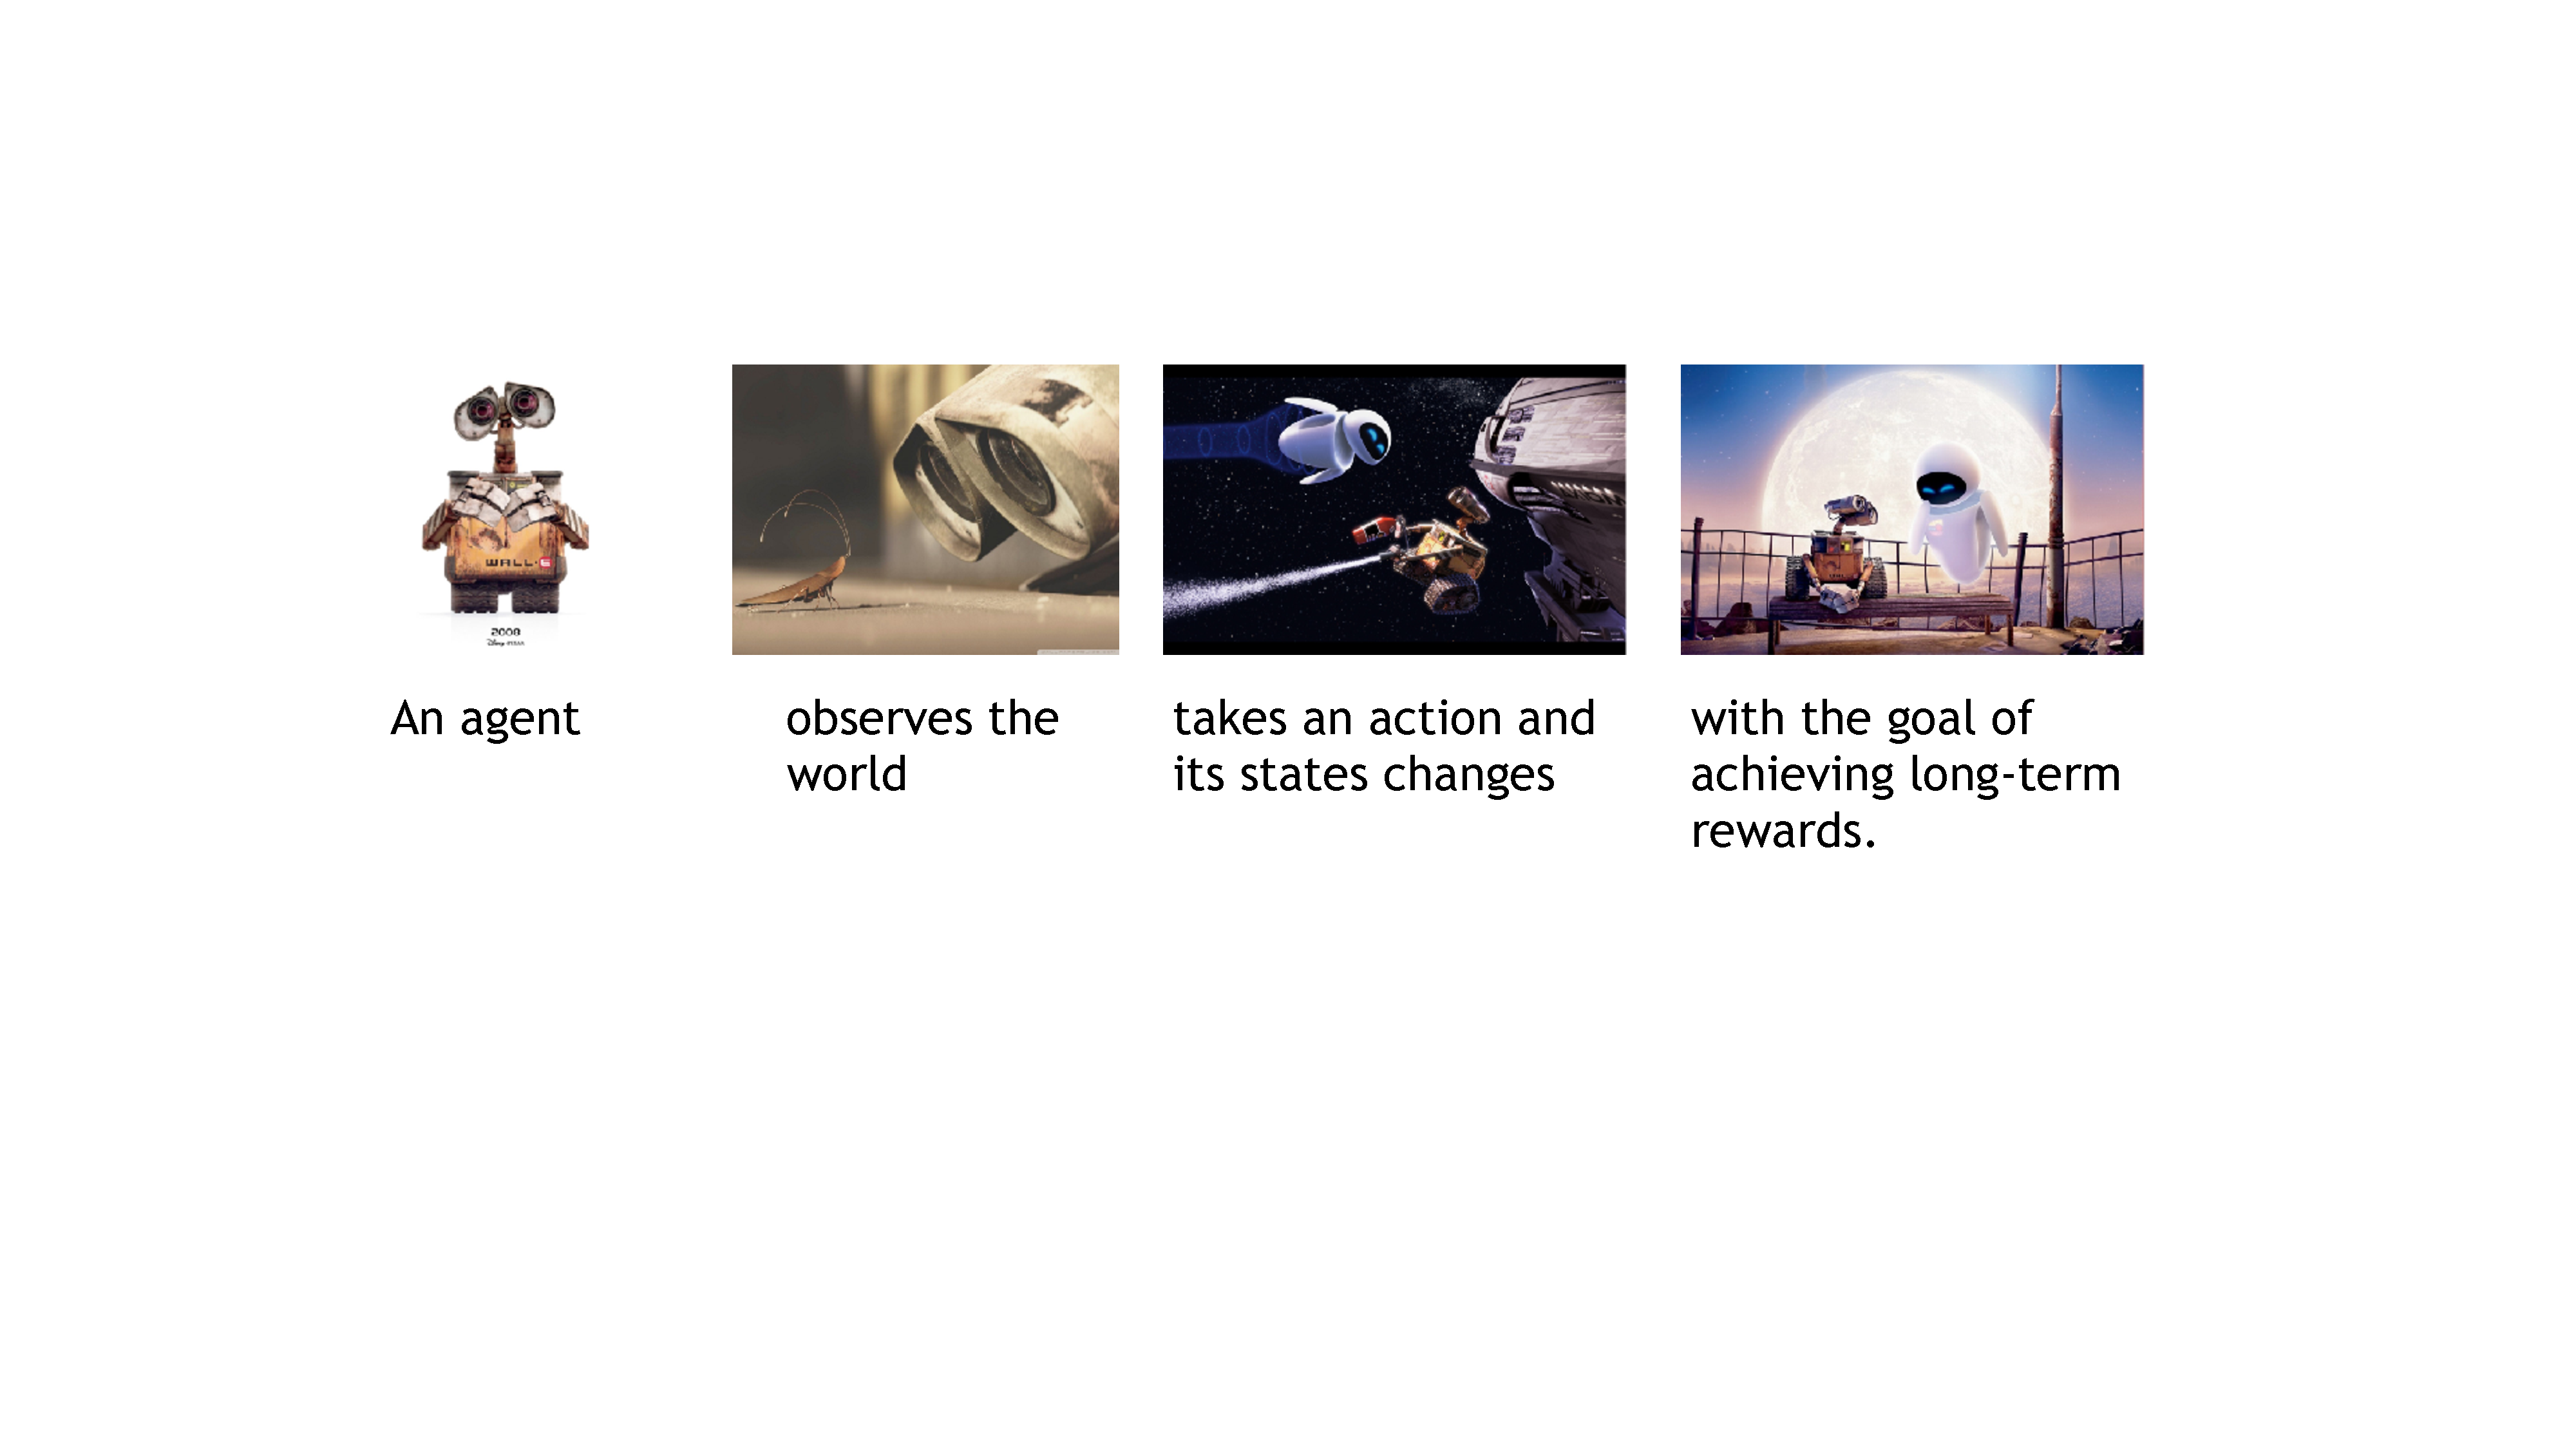
\includegraphics[width=0.75\linewidth]{Figures/RL_Problem}
\end{figure}

Reinforcement Learning Problem: An agent continually interacts with the environment. How should it choose its actions so that its long-term rewards are maximized?	
\end{frame}



%%%%%%%%%%%%%%%%%%%%%%%%%%%%%%%%%%%%%%%%%%%% 

\begin{frame}\frametitle{Playing Games: Atari}\small
\begin{figure}
\href{run:videos/intro/deep_mind.mp4}{
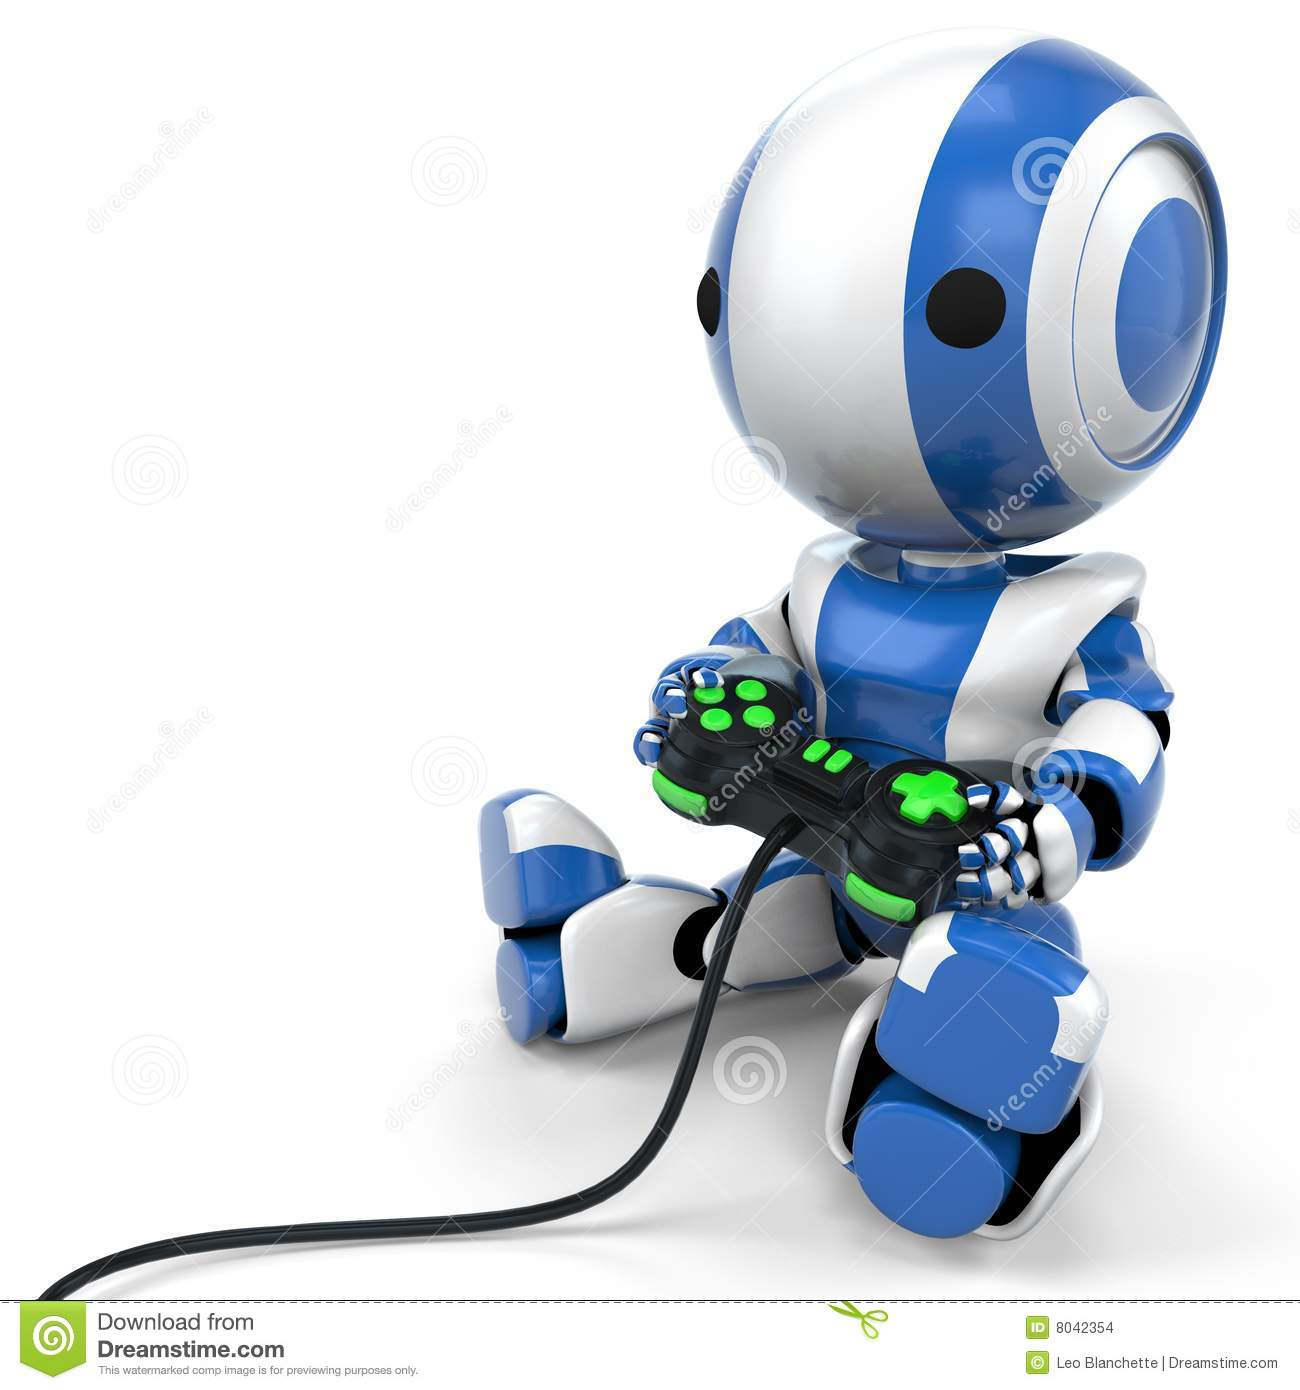
\includegraphics[width =0.6\linewidth,trim=0 69 0 0,clip]{Figures/robot_game.jpg}\\
{\color{magenta}{\url{https://www.youtube.com/watch?v=V1eYniJ0Rnk}}}
}
\end{figure}
\end{frame}

\begin{frame}\frametitle{Playing Games: Super Mario}\small
\begin{figure}
\href{run:videos/intro/super_mario.mp4}{
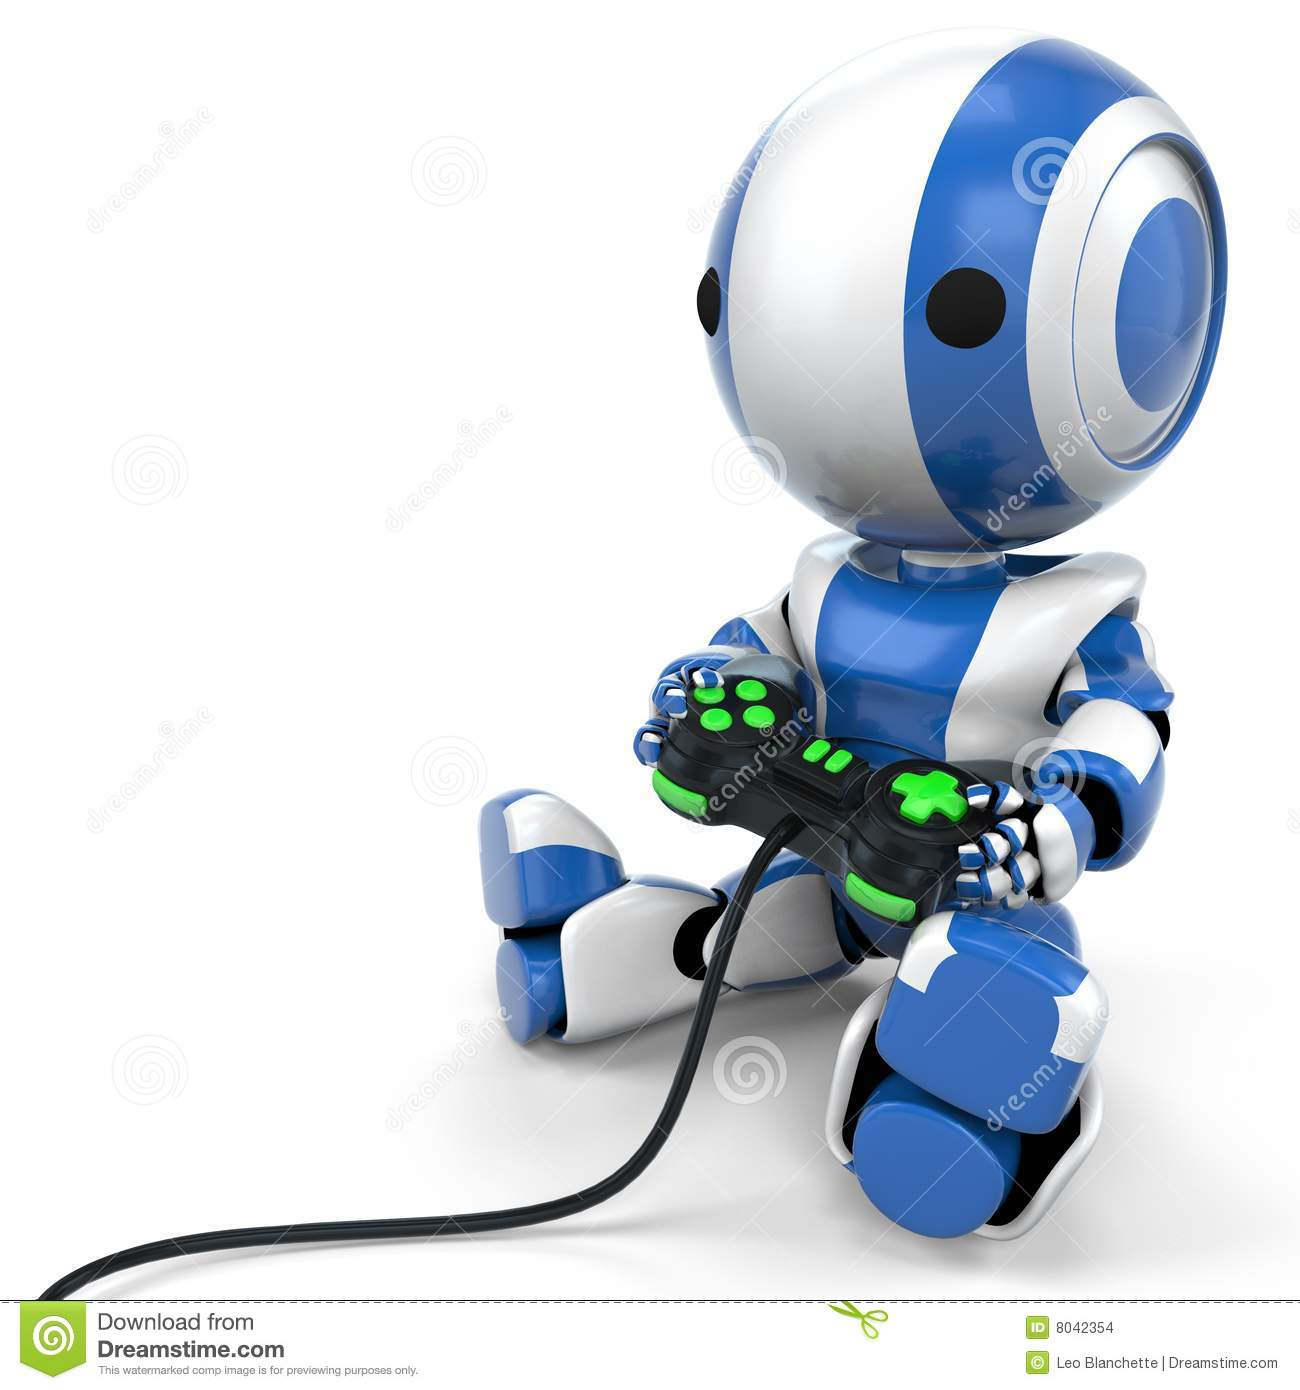
\includegraphics[width =0.6\linewidth,trim=0 69 0 0,clip]{Figures/robot_game.jpg}\\
{\color{magenta}{\url{https://www.youtube.com/watch?v=wfL4L_l4U9A}}}
}
\end{figure}
\end{frame}

\begin{frame}\frametitle{Making Pancakes!}\small
\begin{figure}
\href{run:videos/lecture19/pancakes.mp4}{
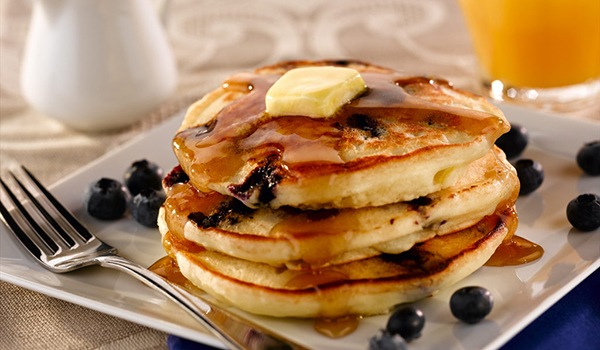
\includegraphics[width=0.9\linewidth]{Figures/pancakes1}\\
{\color{magenta}{\url{https://www.youtube.com/watch?v=W_gxLKSsSIE}}}
}
\end{figure}
\end{frame}


\begin{frame}\frametitle{Reinforcement Learning Resources}\small
\begin{itemize}

\item {\it Reinforcement Learning: An Introduction second edition}, Sutton \& Barto Book (2018)
\item  \href{https://www.youtube.com/watch?v=2pWv7GOvuf0}{Video lectures by David Silver}
\end{itemize}
\end{frame}

% \begin{frame}\frametitle{What is Reinforcement Learning?}\small
% \begin{figure}
% 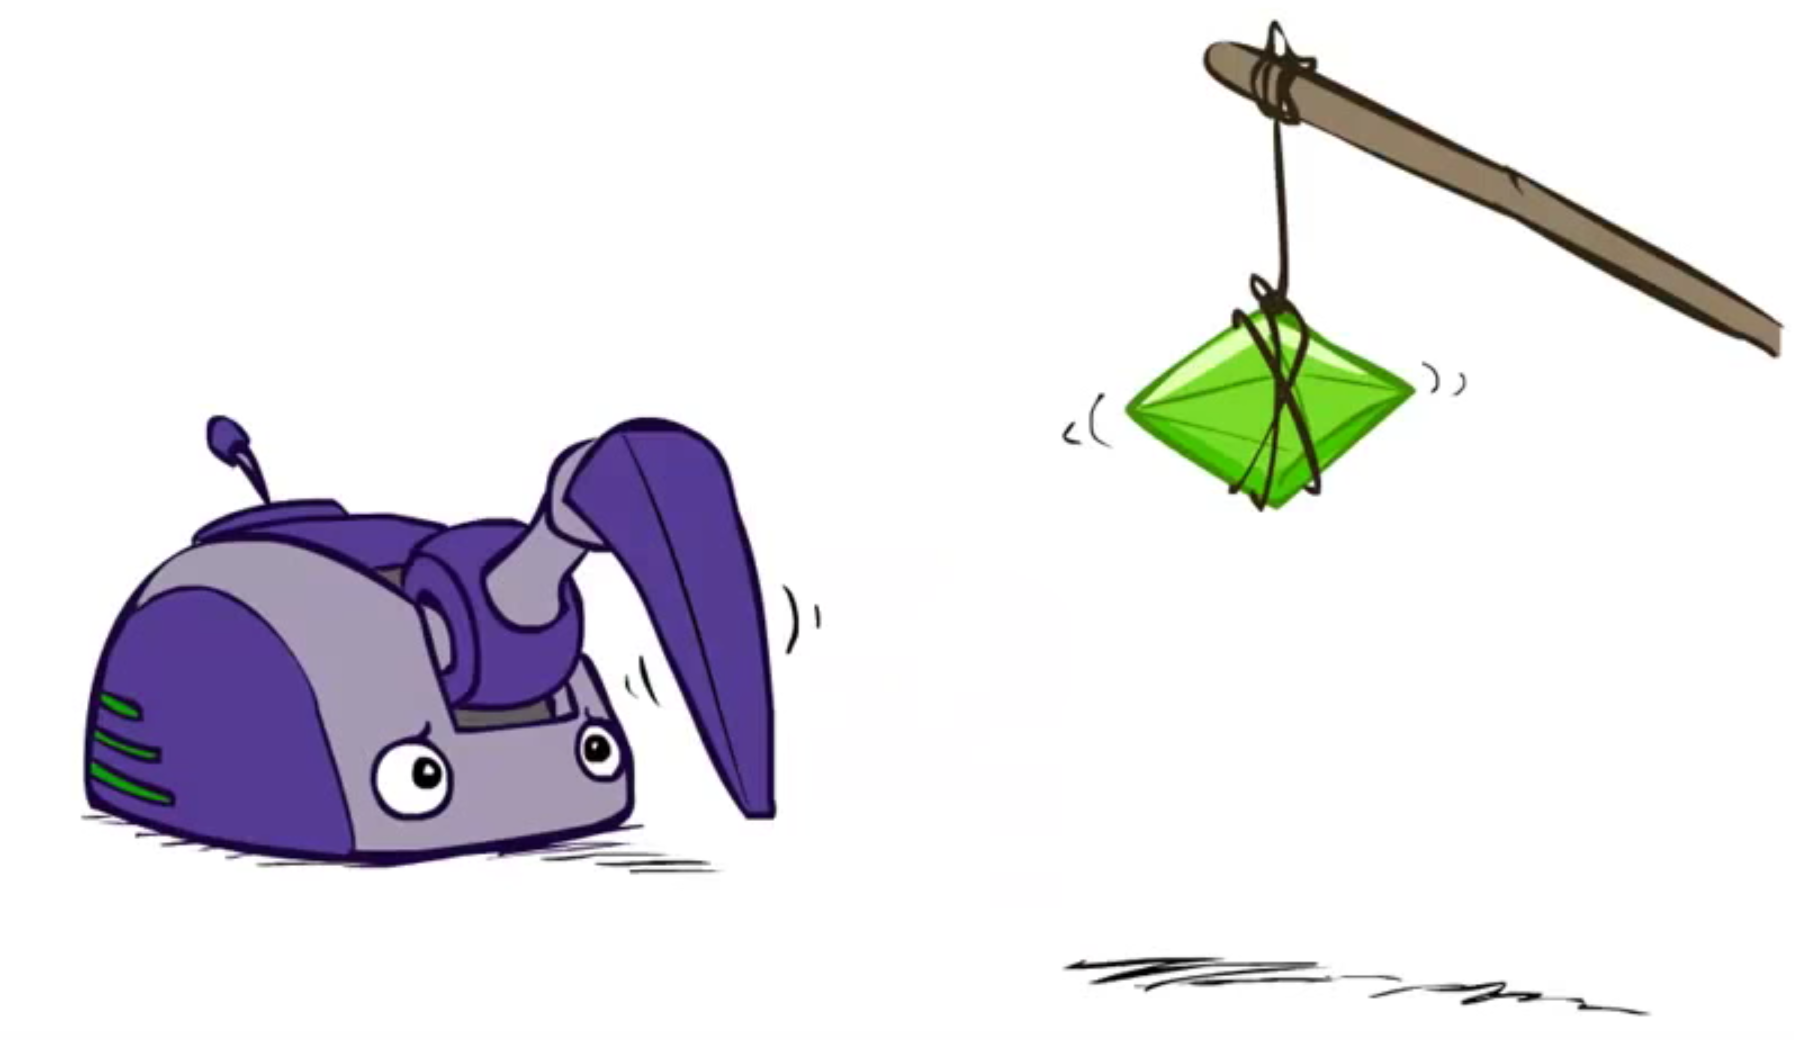
\includegraphics[width=0.9\linewidth]{../old_course_material/slides/figs/lecture19/rll2}
% \end{figure}
% \vspace{5mm}
% \scriptsize [pic from: Peter Abbeel]
% \end{frame}
% 

\begin{frame}\frametitle{Reinforcement Learning}\small
\begin{itemize}
\item Learning algorithms differ in the information available to learner
\begin{itemize}
\setlength\itemsep{1em}
\onslide<2->\item \high{Supervised}: correct outputs, e.g., class label
\onslide<3->\item \high{Unsupervised}: no feedback, must construct measure of good output
\onslide<4->\item \high{Reinforcement learning}: Reward (or cost)
\end{itemize}
\onslide<5->\item More realistic learning scenario: 
\begin{itemize}
\setlength\itemsep{1em}
\item Continuous stream of input information, and actions\\[0.7mm] 
\onslide<6->\item Effects of action depend on state of the world\\[0.7mm] 
\onslide<7->\item Obtain reward that depends on world state and actions\\[0.7mm] 
\begin{itemize}
\onslide<8->\item You know the reward for your action, not other actions.
\onslide<9->\item Could be a delay between action and reward.
\end{itemize}
\end{itemize}
\end{itemize}
\end{frame}

\begin{frame}\frametitle{Reinforcement Learning}\small
%\vspace{8mm}

\begin{figure}
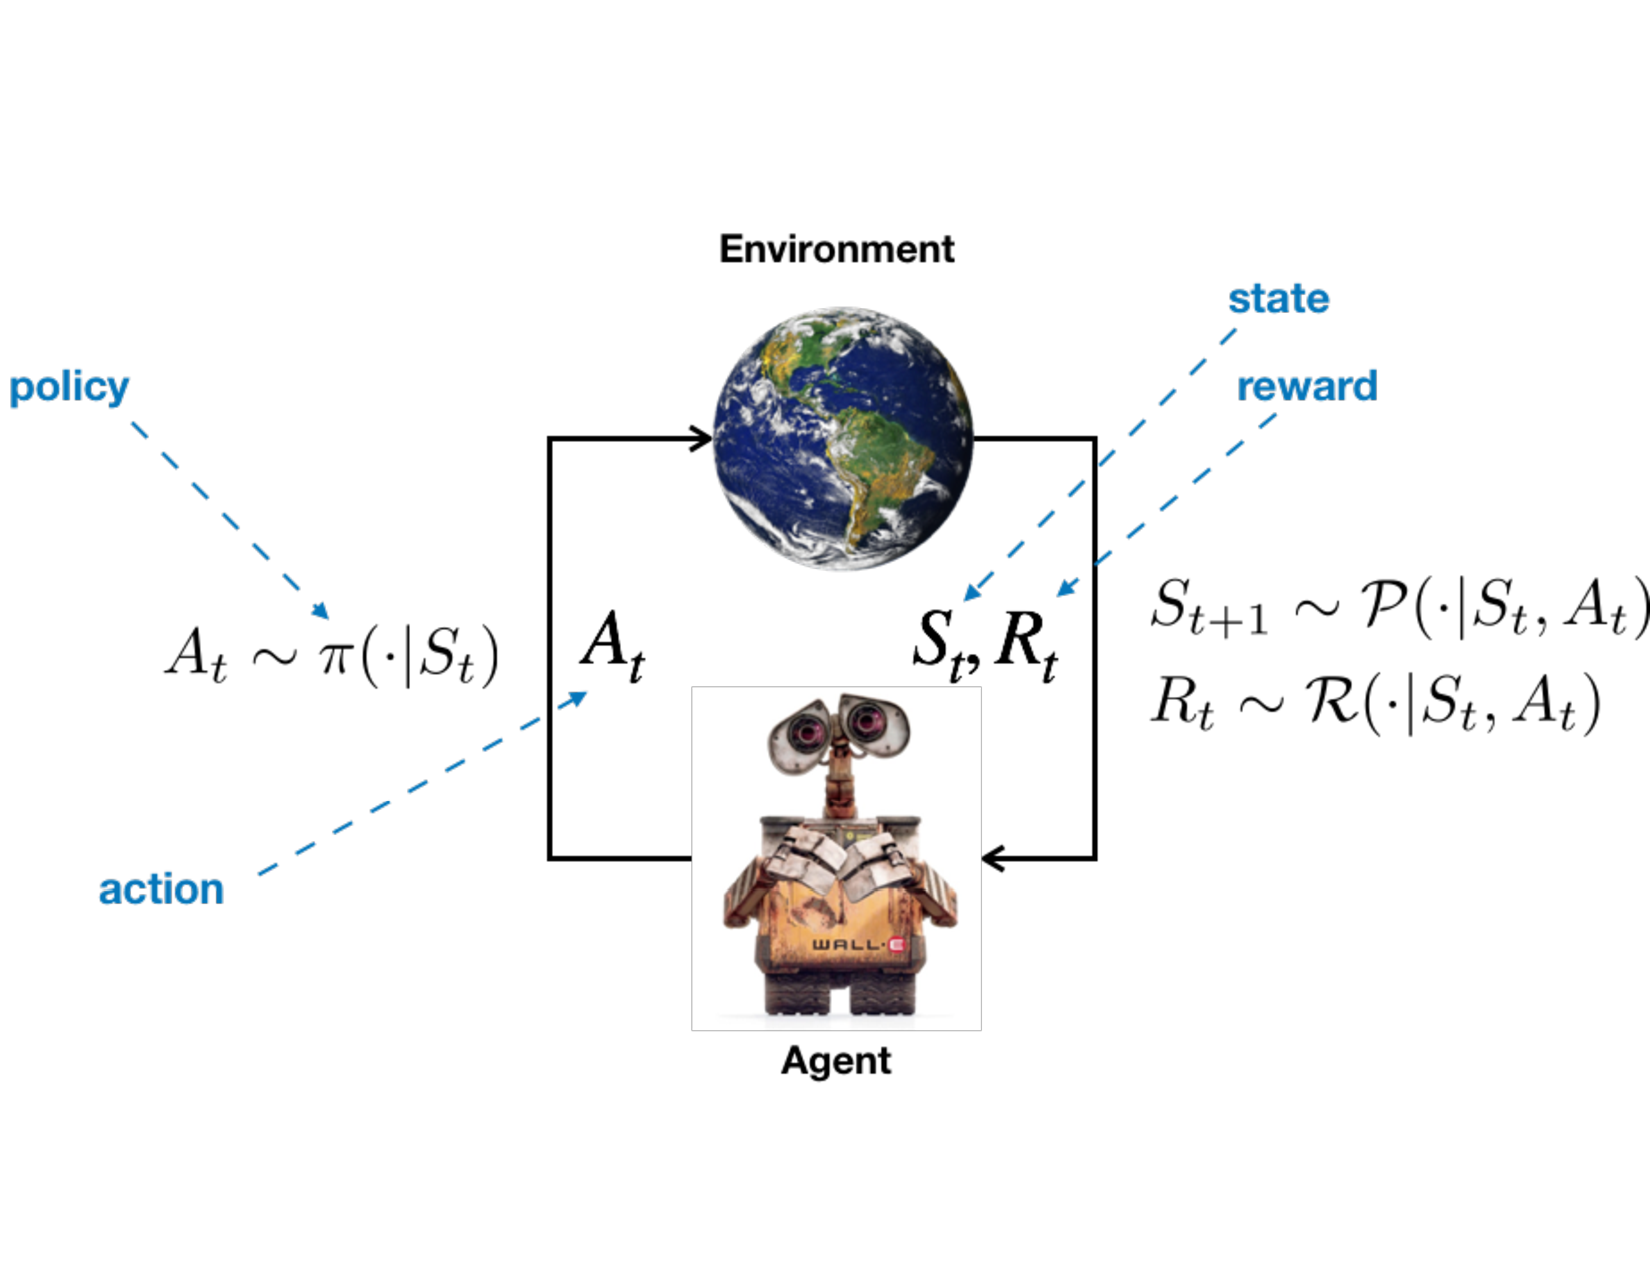
\includegraphics[width=0.85\linewidth]{Figures/RL_agent}
\end{figure}

%\begin{figure}
%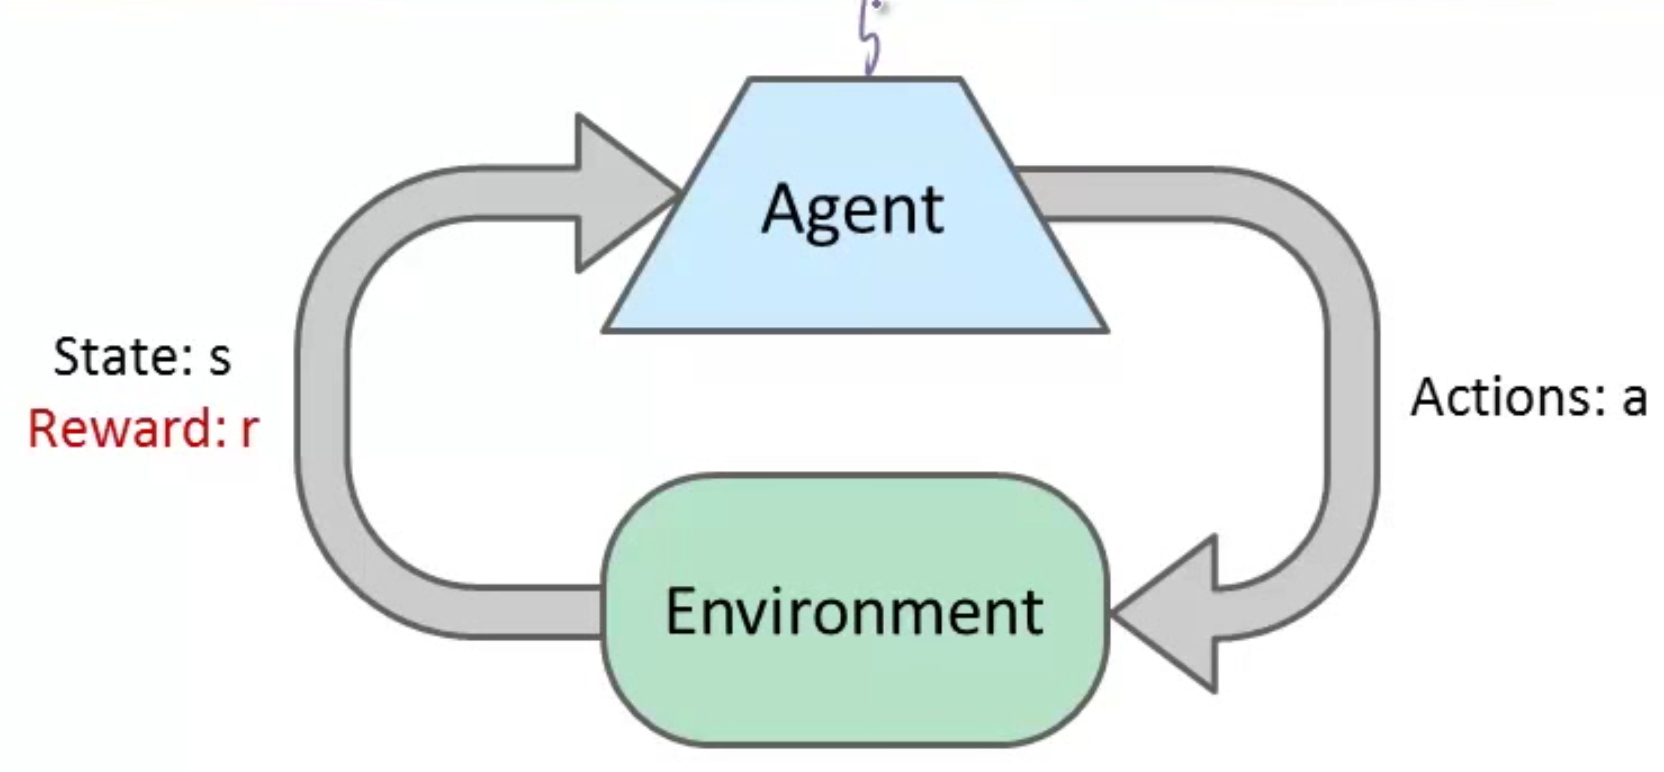
\includegraphics[width=0.85\linewidth]{Figures/rll3}
%\end{figure}
%\vspace{7mm}
%
%\scriptsize [pic from: Peter Abbeel]
\end{frame}

\begin{frame}\frametitle{Example: Tic Tac Toe, Notation}\small
\vspace{4mm}
\begin{figure}
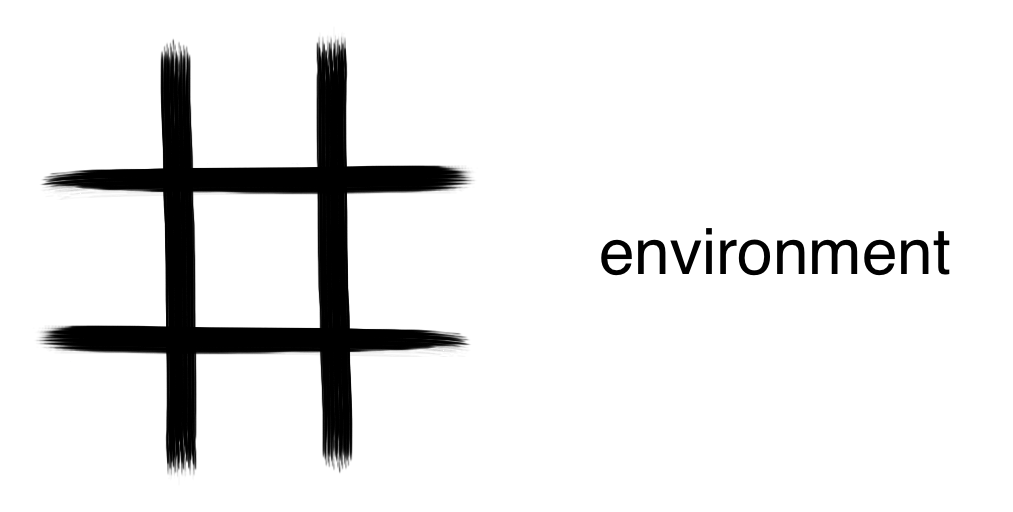
\includegraphics[width=0.75\linewidth]{Figures/tic1d}
\end{figure}
\vspace{5mm}
\end{frame}

\begin{frame}\frametitle{Example: Tic Tac Toe, Notation}\small
\vspace{4mm}

\begin{figure}
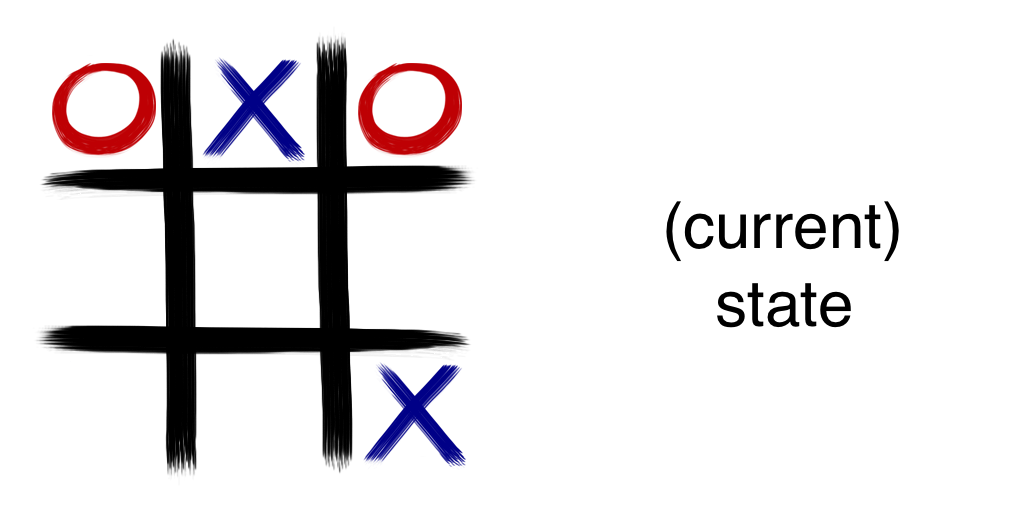
\includegraphics[width=0.75\linewidth]{Figures/tic1c}
\end{figure}
\vspace{5mm}
\end{frame}

\begin{frame}\frametitle{Example: Tic Tac Toe, Notation}\small
\vspace{4mm}

\begin{figure}
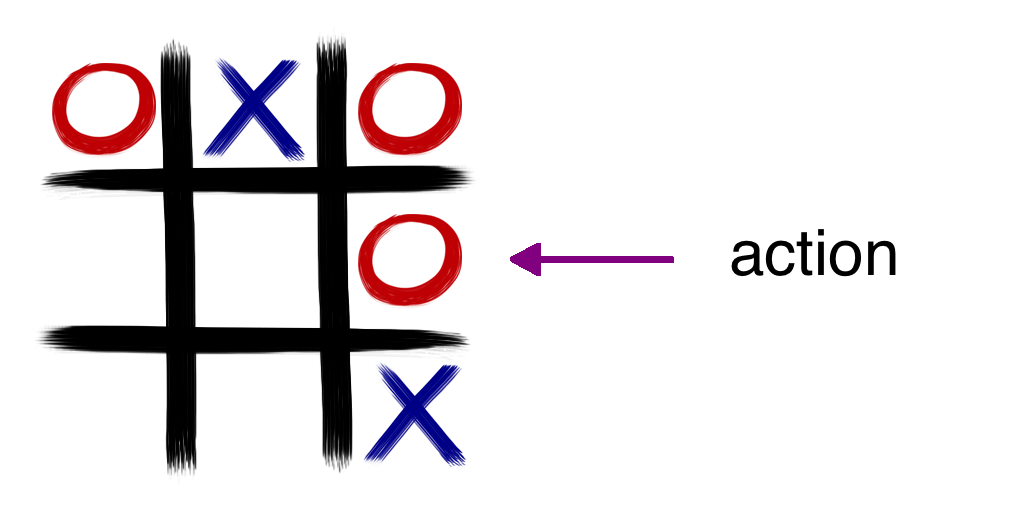
\includegraphics[width=0.75\linewidth]{Figures/tic1b}
\end{figure}
\vspace{5mm}
\end{frame}

\begin{frame}\frametitle{Example: Tic Tac Toe, Notation}\small
\vspace{4mm}

\begin{figure}
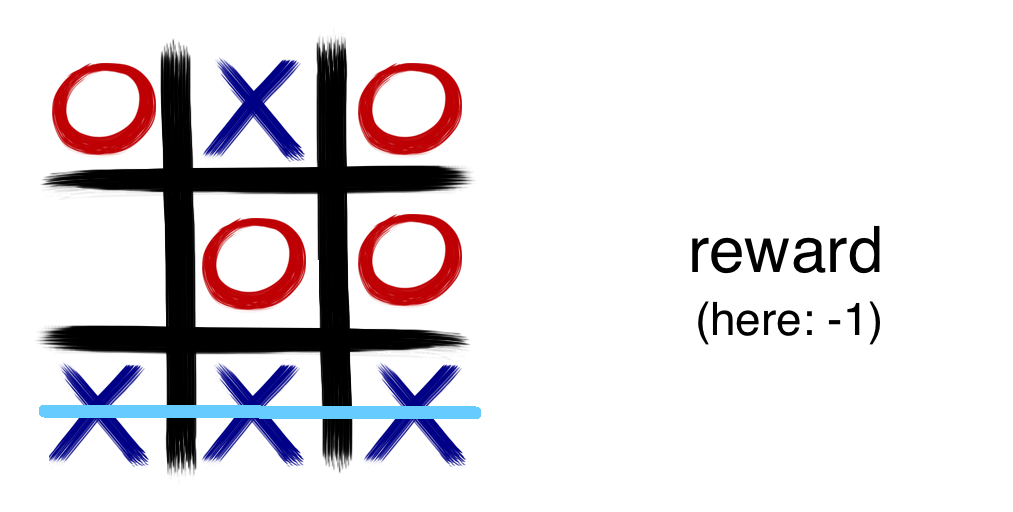
\includegraphics[width=0.75\linewidth]{Figures/tic1e}
\end{figure}
\vspace{5mm}
\end{frame}


%%%%%%%%%%%%%%%%%%%%%%%%%%%%%%%%%%%%%%%%%%%% 
\begin{frame}\frametitle{Formalizing Reinforcement Learning Problems}\small
\begin{itemize}
\item Markov Decision Process (MDP) is the mathematical framework to describe RL problems
\item A discounted MDP is defined by a tuple $(\States, \Actions, \PKernel, \RKernel, \gamma)$.
\begin{itemize}
	\item $\States$: State space. Discrete or continuous
	\item $\Actions$: Action space. Here we consider finite action space, i.e., $\Actions = \{a_1, \dotsc, a_{|\Actions|} \}$.
	\item $\PKernel$: Transition probability
	\item $\RKernel$: Immediate reward distribution
	\item $\gamma$: Discount factor ($0 \leq \gamma < 1$)
\end{itemize}
\end{itemize}

\end{frame}


%%%%%%%%%%%%%%%%%%%%%%%%%%%%%%%%%%%%%%%%%%%% 
\begin{frame}\frametitle{Formalizing Reinforcement Learning Problems}\small
\begin{itemize}
\item The agent has a \high{state} $s \in \mathcal{S}$ in the environment, e.g., the location of X and O in tic-tac-toc, or the location of a robot in a room.
\item At every time step $t = 0, 1, \dotsc$, the agent is at state $s_t$.
	\begin{itemize}
	\item Takes an \high{action} $a_t$
	\item Moves into a new state $s_{t+1}$, according to the dynamics of the environment and the selected action, i.e., $s_{t+1} \sim \PKernel(\cdot|s_t, a_t)$
	\item Receives some \high{reward} $r_{t+1} \sim \RKernel(\cdot|s_t, a_t, s_{t+1})$
	\end{itemize}
\end{itemize}

\begin{figure}
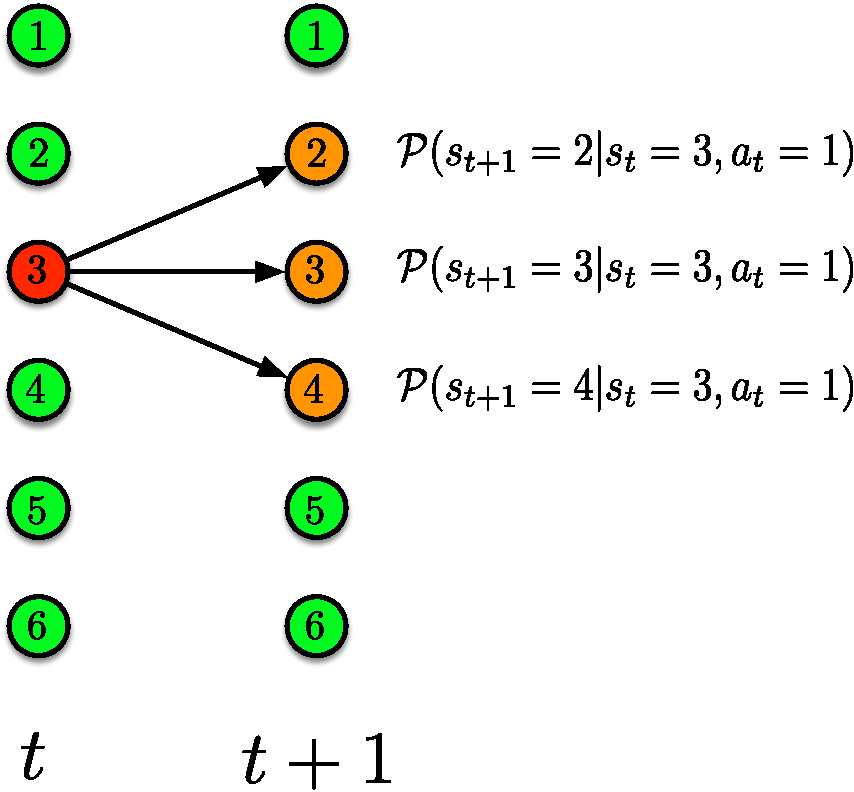
\includegraphics[width=0.3\linewidth]{Figures/MDP_transition}
\end{figure}

\end{frame}




%%%%%%%%%%%%%%%%%%%%%%%%%%%%%%%%%%%%%%%%%%%% 
\begin{frame}\frametitle{Formulating Reinforcement Learning}\small

%\begin{figure}
%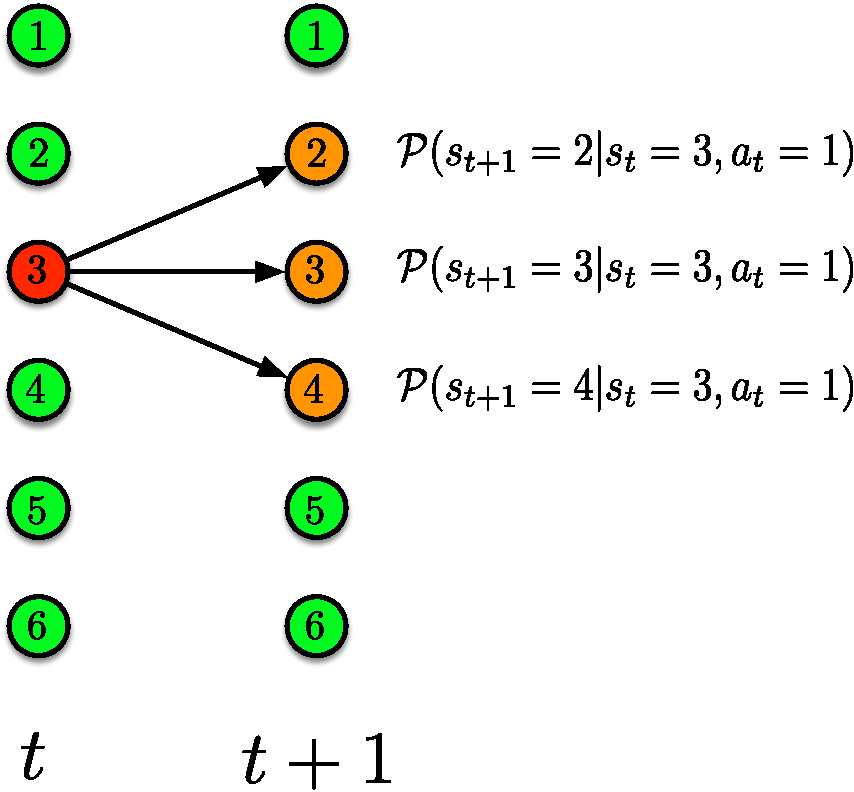
\includegraphics[width=0.1\linewidth]{Figures/MDP_transition}
%\end{figure}

\begin{itemize}
\item The action selection mechanism is described by a \high{policy} $\pi$
\begin{itemize}
\item Policy $\pi$ is a mapping from states to actions, i.e., $a_t = \pi(s_t)$
\end{itemize}
\item The goal is to find a policy $\pi$ such that \high{long-term rewards} of the agent is maximized. 
\item Different notations of long-term reward:
	\begin{itemize}
	\item
	Average reward:
	\[
	r_{t}+r_{t+1}+r_{t+2}+\dots
	\]
	\item Sometimes a future reward is discounted by $\gamma^{k-1}$, where $k$ is the number of time-steps in the future when it is received:
		\[
	r_{t}+\gamma r_{t+1}+\gamma^2 r_{t+2}+\dots
	\]
		\begin{itemize}
			\item If $\gamma$ close to $1$, rewards further in the future count more, and we say that the agent is ``farsighted''
			\item $\gamma$ is less than $1$ because there is usually a time limit to the sequence of actions needed to solve a task (we prefer rewards sooner rather than 
		\end{itemize}
	\end{itemize}
\end{itemize}
\end{frame}


%%%%%%%%%%%%%%%%%%%%%%%%%%%%%%%%%%%%%%%%%%% 
\begin{frame}\frametitle{Transition Probability (or Dynamics)}\small
\begin{itemize}
\item The transition probability describes the changes in the state of the agent when it chooses actions
\[
	\PKernel(s_{t+1}=s', r_{t+1}=r' | s_t = s, a_t = a)
\]
%
\item This model has \high{Markov property}: the future depends on the past only through the current state
%
\end{itemize}
\begin{figure}
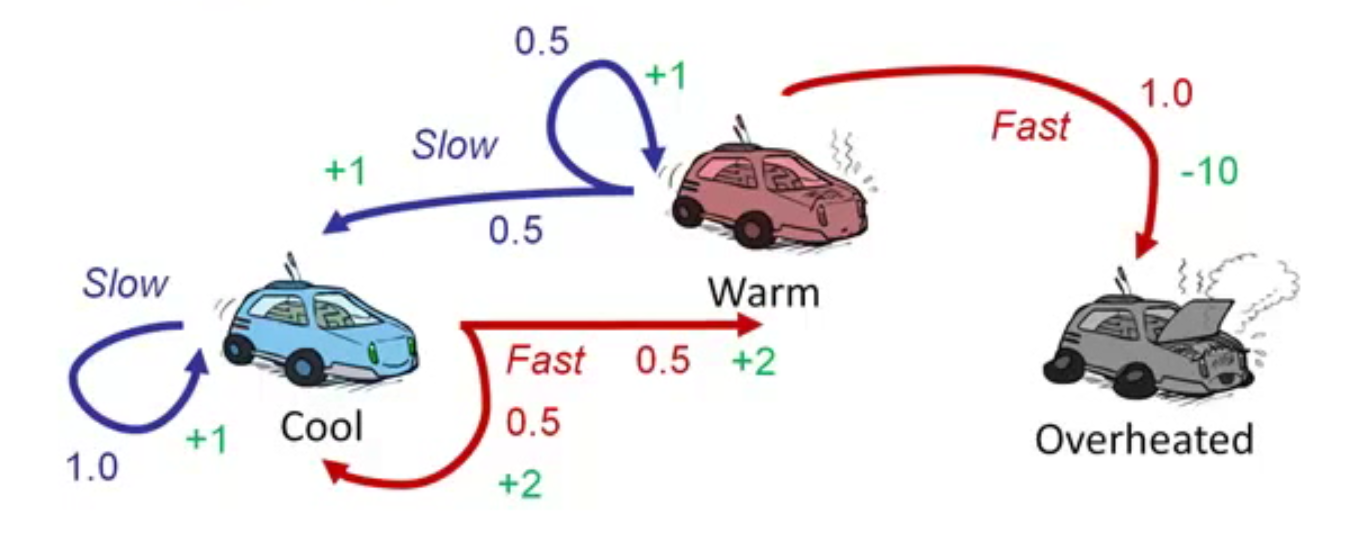
\includegraphics[width=0.7\linewidth]{Figures/rll6} 
\end{figure}
\end{frame}


%%%%%%%%%%%%%%%%%%%%%%%%%%%%%%%%%%%%%%%%%%% 
\begin{frame}\frametitle{Policy}\small
\begin{itemize}
\item A \high{policy} is the action selection mechanism of the agent, and describes its behaviour.
\item Policy can be deterministic or stochastic:
	\begin{itemize}
		\item Deterministic policy: $a = \pi(s)$
		\item Stochastic policy: $A \sim \pi(\cdot|s)$
	\end{itemize}
\end{itemize}

\end{frame}


%%%%%%%%%%%%%%%%%%%%%%%%%%%%%%%%%%%%%%%%%%% 
\begin{frame}\frametitle{Value Function}\small
\begin{itemize}
\item \high{Value function} is the expected future reward, and is used to evaluate the desirability of states.
\item State-value function $\Vpi$ (or simply value function) for policy $\pi$ is a function defined as
\begin{align*}
	\Vpi(s) \eqdef \EEX{\pi}{\sum_{t \geq 0} \gamma^t R_t \mid S_0 = s}.
\end{align*}
It describes the expected discounted reward if the agent starts from state $s$ and follows policy $\pi$.

\item The action-value function $\Qpi$ for policy $\pi$ is
\begin{align*}
	\Qpi(s,a) \eqdef \EEX{\pi}{\sum_{t \geq 0} \gamma^t R_t \mid S_0 = s, A_0 = a}.
\end{align*}
It describes the expected discounted reward if the agent starts from state $s$, takes action $a$, and afterwards follows policy $\pi$.

\end{itemize}

\end{frame}

%%%%%%%%%%%%%%%%%%%%%%%%%%%%%%%%%%%%%%%%%%% 
\begin{frame}\frametitle{Value Function}\small

\begin{itemize}

	\item Our aim will be to find a policy $\pi$ that maximizes the value function (the total reward we receive over time): find the policy with the highest expected reward


	\item Optimal value function:
	\[
	  \Qopt(s,a) = \sup_\pi \Qpi(s,a)
	\]

	\item Given $\Qopt$, the optimal policy can be obtained as
	\[
	  \piopt(s) \leftarrow \argmax_a \Qopt(s,a)
	\]

	\item The goal of an RL agent is to find a policy $\pi$ that is close to optimal, i.e., $\Qpi \approx \Qopt$.
\end{itemize}

\end{frame}



%%%%%%%%%%%%%%%%%%%%%%%%%%%%%%%%%%%%%%%%%%% 
\begin{frame}\frametitle{Bellman Equation}\small
The value function satisfies the following recursive relationship:
\begin{align*}
  \Qpi(s,a) & = \EE{\sum_{t=0}^\infty \gamma^t R_t | S_0 = s, A_0 = a }
  \\
  &
  = \EE{R(S_0, A_0) + \gamma \sum_{t = 0}^\infty \gamma^t R_{t+1} | s_0 = s, a_0 = a }
  \\
  &  
  = \EE{R(S_0, A_0) + \gamma \Qpi(S_1, \pi(S_1)) | S_0 = s, A_0 = a }
  \\
  &
  =
  \underbrace{
  r(s,a) + \gamma \int_\States \PKernel(\ds' | s, a) \Qpi (s', \pi(s')) }_{\eqdef (\Tpi \Qpi)(s,a) }
\end{align*}


This is called the Bellman equation and $\Tpi: B(\SA) \ra B(\SA)$ is the Bellman operator.
Similarly, we define the Bellman \emph{optimality} operator:
\begin{align*}
  (\Topt Q)(s,a) \eqdef r(s,a) + \gamma \int_\States \PKernel(\ds' | s,a) \max_{a' \in \Actions} Q(s',a')
\end{align*}
\end{frame}


%%%%%%%%%%%%%%%%%%%%%%%%%%%%%%%%%%%%%%%%%%% 
\begin{frame}\frametitle{Bellman Equation}\small

\begin{itemize}

	\item Key observation:
	\begin{align*}
	  & \Qpi = \Tpi \Qpi \\
	  & \Qopt = \Topt \Qopt
	\end{align*}

	\item Value-based approaches try to find a $\Qhat$ such that
	\[
	  \Qhat \approx \Topt \Qhat
	\]

	\item The greedy policy of $\Qhat$ is close to the optimal policy:
	\[
		  % Q^{\pi(x;\Qhat)} \approx Q^{\piopt} = \Qopt
		  Q^{\pi(x;\Qhat)} \approx \Qopt
	\]
	where the greedy policy is defined as
	\[
	  \pi(s; \Qhat) \leftarrow \argmax_{a \in \Actions} \Qhat(s,a)
	\]
\end{itemize}
\end{frame}


%%%%%%%%%%%%%%%%%%%%%%%%%%%%%%%%%%%%%%%%%%% 
\begin{frame}\frametitle{Finding the Optimal Value Function: Value Iteration}\small
\begin{itemize}
	\item Assume that we know the model $\PKernel$ and $\RKernel$. How can we find the optimal value function?
	\item This is the problem of \high{Planning}.
	\item We can benefit from the Bellman optimality equation and use a method called \high{Value Iteration}
		\[
			Q_{k+1} \leftarrow \Topt Q_k
		\]
	\begin{figure}
		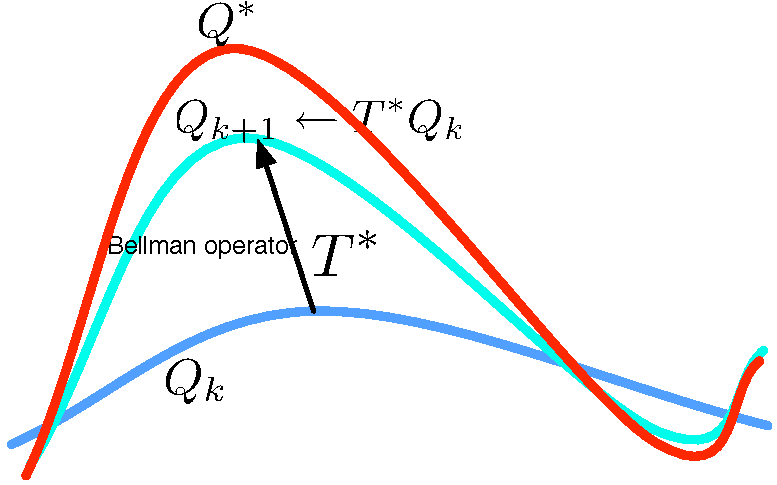
\includegraphics[width=0.4\linewidth]{Figures/VI} 
	\end{figure}
\end{itemize}
\vspace{-0.5cm}
\begin{align*}
	&
	Q_{k+1}(s,a) \leftarrow r(s,a) + \gamma \int_{\States} \PKernel(\ds' | s,a) \max_{a' \in \AA} Q_k(s',a')
	\\
	& Q_{k+1}(s,a) \leftarrow r(s,a) + \gamma \sum_{s' \in \States} \PKernel(s' | s,a) \max_{a' \in \AA} Q_k(s',a')
\end{align*}



\end{frame}



%%%%%%%%%%%%%%%%%%%%%%%%%%%%%%%%%%%%%%%%%%% 
\begin{frame}\frametitle{Value Iteration}\small
\begin{itemize}
	\item The Value Iteration converges to the optimal value function.
	\item This is because of the contraction property of the Bellman (optimality) operator, i.e., $\norm{\Topt Q_1 - \Topt Q_2}_\infty \leq \gamma \norm{Q_1 - Q_2}_\infty$.
\end{itemize}
	\begin{figure}
		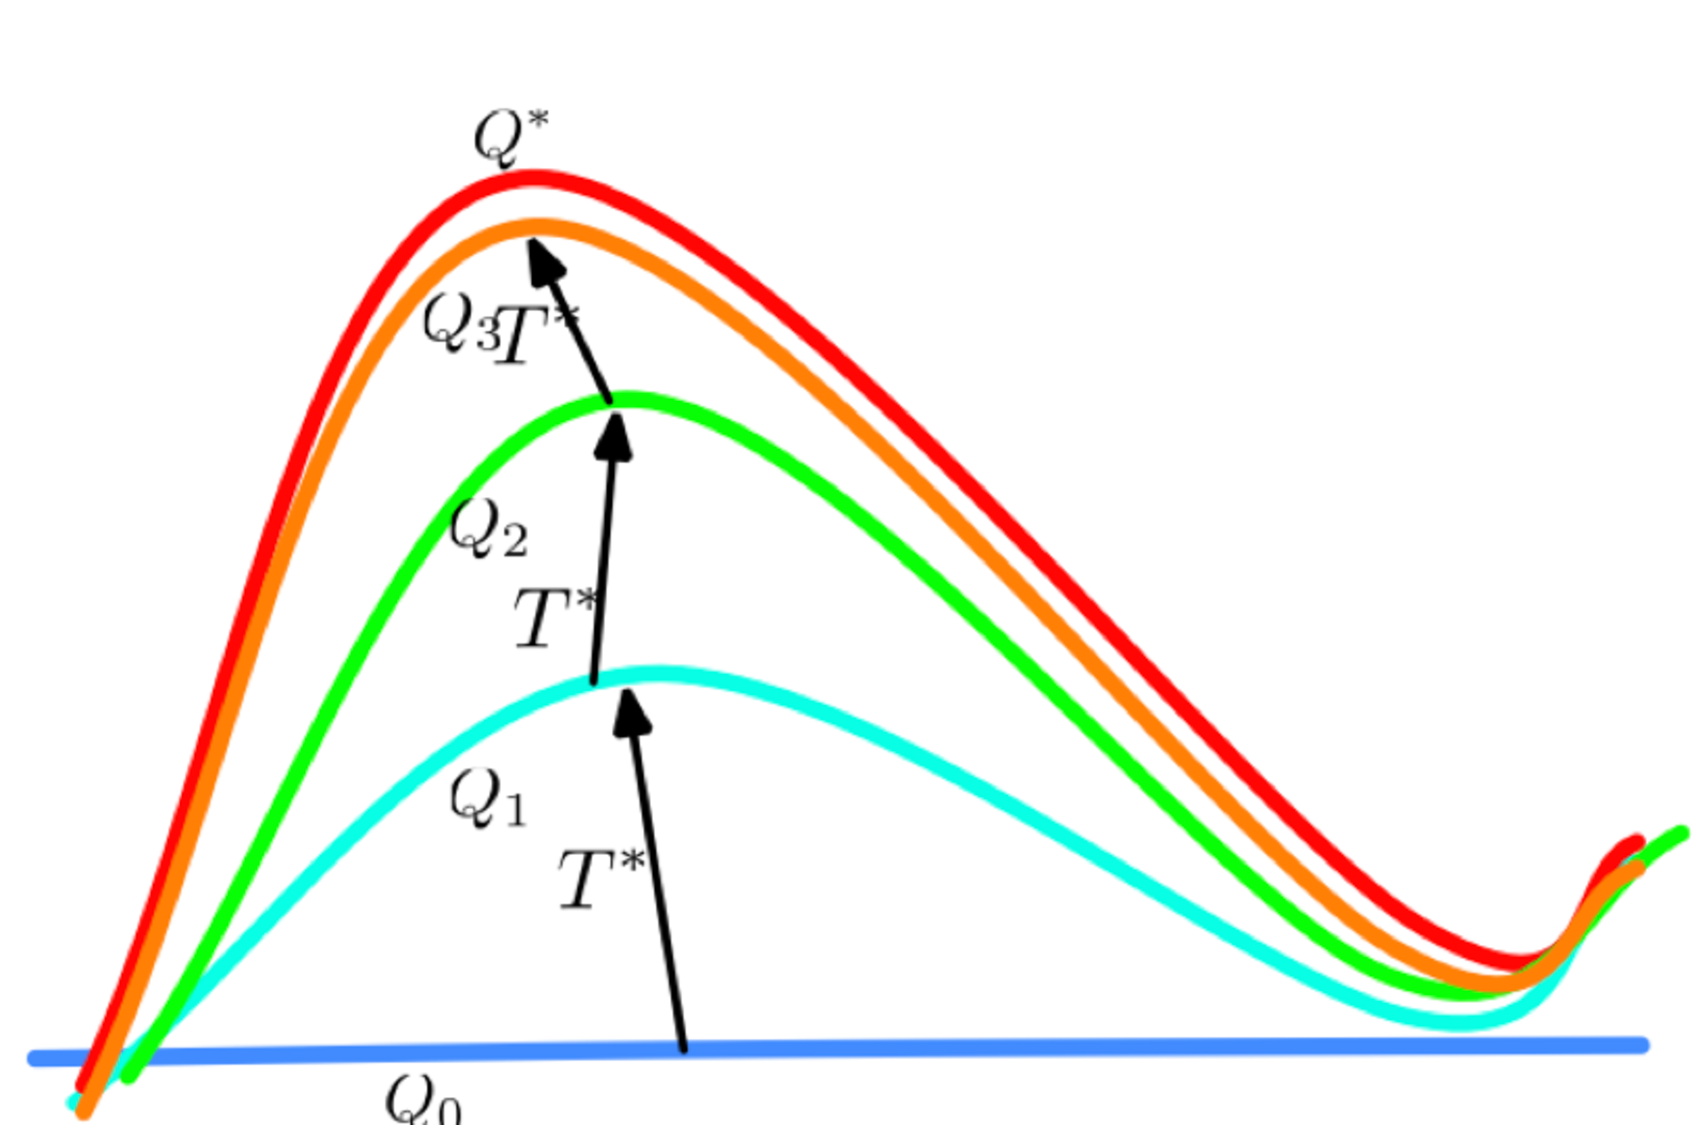
\includegraphics[width=0.4\linewidth]{Figures/VI_Convergence} 
		\vspace{-0.2in}
	\end{figure}
\[
	Q_{k+1} \leftarrow \Topt Q_k
\]


\begin{align*}
	&
	Q_{k+1}(s,a) \leftarrow r(s,a) + \gamma \int_{\States} \PKernel(\ds' | s,a) \max_{a' \in \AA} Q_k(s',a')
	\\
	& Q_{k+1}(s,a) \leftarrow r(s,a) + \gamma \sum_{s' \in \States} \PKernel(s' | s,a) \max_{a' \in \AA} Q_k(s',a')
\end{align*}



\end{frame}



\begin{frame}\frametitle{Maze Example}\small
\begin{figure}
\begin{minipage}{0.5\linewidth}
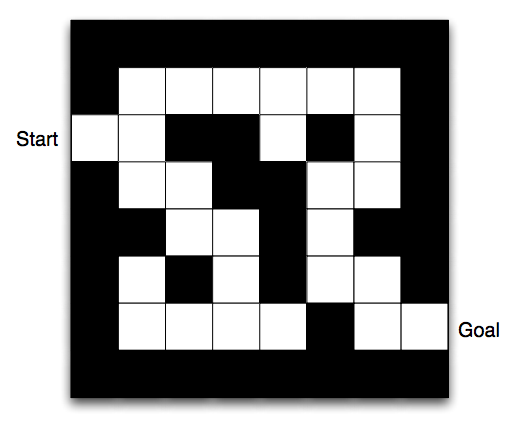
\includegraphics[width=\linewidth]{Figures/maze1}
\end{minipage}
\hspace{3mm}
\begin{minipage}{0.45\linewidth}
\begin{itemize}
\item Rewards: \onslide<2-> $-1$ per time-step
\item Actions: \onslide<3-> N, E, S, W
\item States: \onslide<4-> Agent's location
\end{itemize}
\end{minipage}
\end{figure}

\vspace{12mm}
\scriptsize [Slide credit: D. Silver]
\end{frame}

\begin{frame}\frametitle{Maze Example}\small
\begin{figure}
\begin{minipage}{0.5\linewidth}
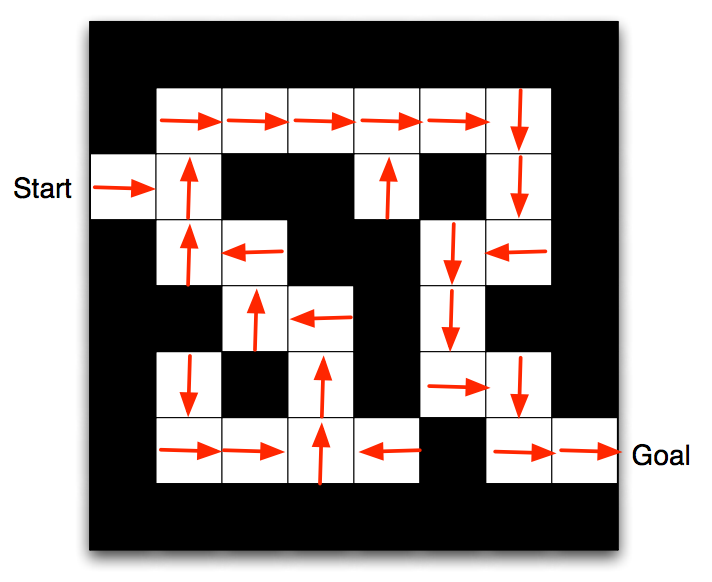
\includegraphics[width=\linewidth]{Figures/maze2}
\end{minipage}
\hspace{3mm}
\begin{minipage}{0.45\linewidth}
\begin{itemize}
\item Arrows represent policy $\pi(s)$ for each state $s$
\end{itemize}
\end{minipage}
\end{figure}

\vspace{14mm}
\scriptsize [Slide credit: D. Silver]
\end{frame}

\begin{frame}\frametitle{Maze Example}\small
\begin{figure}
\begin{minipage}{0.5\linewidth}
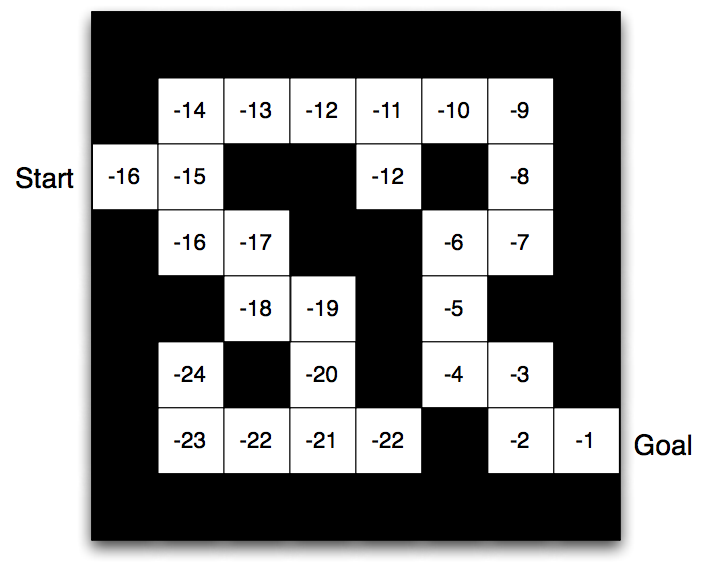
\includegraphics[width=\linewidth]{Figures/maze3}
\end{minipage}
\hspace{3mm}
\begin{minipage}{0.45\linewidth}
\begin{itemize}
\item Numbers represent value $V^{\pi}(s)$ of each state $s$
\end{itemize}
\end{minipage}
\end{figure}

\vspace{14mm}
\scriptsize [Slide credit: D. Silver]
\end{frame}



\begin{frame}\frametitle{Example: Tic-Tac-Toe}\small
\begin{itemize}
\item Consider the game tic-tac-toe:
\begin{itemize}
 \setlength\itemsep{1em}
\onslide<2->\item \high{reward}: \onslide<3-> win/lose/tie the game $(+1/-1/0)$ [only at final move in given game]
\onslide<4->\item \high{state}: \onslide<5->positions of X's and O's on the board
\onslide<6->\item \high{policy}: mapping from states to actions 
\begin{itemize}
\onslide<7->\item based on rules of game: choice of one open position
\end{itemize}
\onslide<8->\item \high{value function}: prediction of reward in future, based    on current state
\end{itemize}
\onslide<9->\item In tic-tac-toe, since state space is tractable, we can use a table to represent value function 
\end{itemize}
\end{frame}

\begin{frame}\frametitle{RL \& Tic-Tac-Toe}\small
%\vspace{-0.3cm}
\begin{itemize}
\item Each board position (taking into account symmetry) has some probability
\end{itemize}
\begin{minipage}{4cm}
\begin{center}
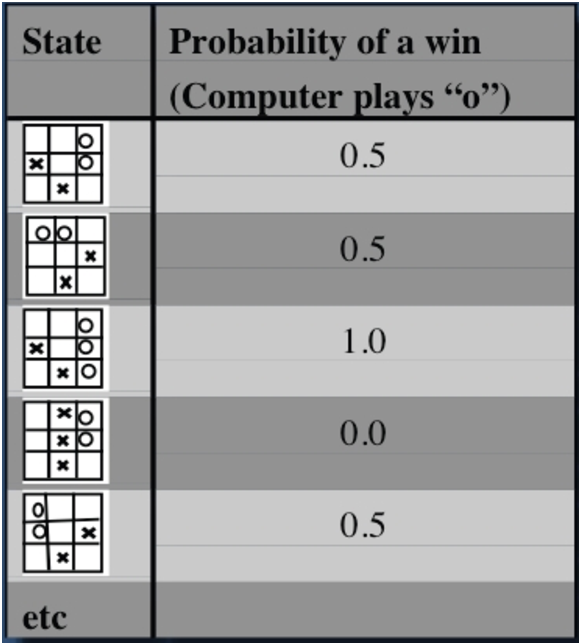
\includegraphics[width=1.0\linewidth]{Figures/tic_tac} 
\end{center}
\end{minipage}
\begin{minipage}{7cm}
\begin{itemize}
%\item Each board position (taking into account symmetry) has some probability
\onslide<2->\item Simple learning process: 
\begin{itemize}
\onslide<3->\item start with all values = 0.5
\onslide<4->\item \high{policy}: choose move with highest probability of winning given current legal moves from current state
\onslide<5->\item update entries in table based on outcome of each game
\onslide<6->\item After many games value function will represent true probability of winning from each state
\end{itemize}
%\item Can try alternative policy: sometimes select moves randomly (exploration)
\end{itemize}
\end{minipage}
\begin{itemize}
\onslide<7->\item Can try alternative policy: sometimes select moves randomly (exploration)
\end{itemize}
\end{frame}



\begin{frame}\frametitle{MDP}\small
\begin{itemize}
\item Markov Decision Problem (MDP): tuple $(S,A,P,\gamma)$ where $P$ is
\[
P(s_{t+1}=s', r_{t+1}=r' | s_t = s, a_t = a)
\]
\onslide<2->\item Main assumption: Markovian dynamics and reward.
\onslide<3->\item Standard MDP problems:
\begin{enumerate}
\onslide<4->\item  \high{Planning}: given complete Markov decision problem as input, compute policy with optimal expected return
\begin{figure}
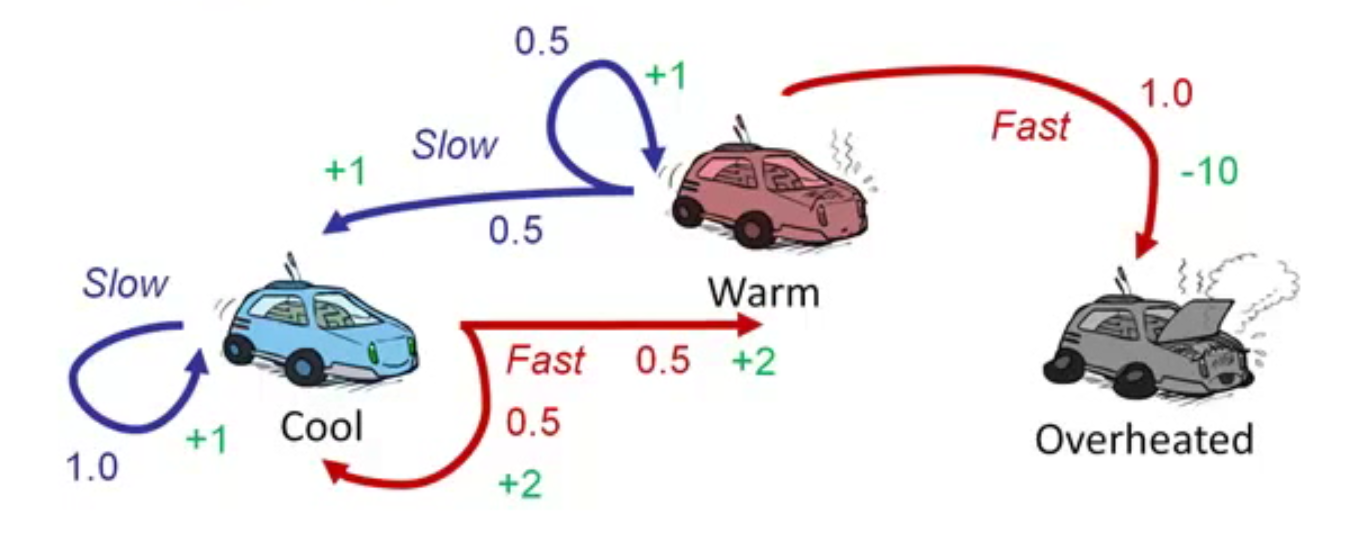
\includegraphics[width=0.7\linewidth]{Figures/rll6} 
\end{figure}
\end{enumerate}
\end{itemize}
\scriptsize [Pic: P. Abbeel]
\end{frame}


\begin{frame}\frametitle{Basic Problems}\small
\begin{itemize}
\item Markov Decision Problem (MDP): tuple $(S,A,P,\gamma)$ where $P$ is
\[
P(s_{t+1}=s', r_{t+1}=r' | s_t = s, a_t = a)
\]
\item Standard MDP problems:
\begin{enumerate}
\item  \high{Planning}: given complete Markov decision problem as input, compute policy with optimal expected return\\[1mm]
\item \high{Learning}: We don't know which states are good or what the actions do. We must try out the actions and states to learn what to do
\end{enumerate}
\end{itemize}
\vspace{28mm}

\scriptsize [P. Abbeel]
\end{frame}

\begin{frame}\frametitle{Example of Standard MDP Problem}\small
\begin{center}
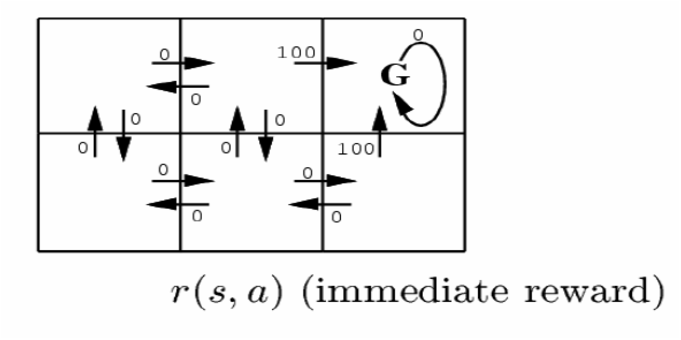
\includegraphics[width=0.54\linewidth]{Figures/tic_tac_rl} 
\end{center}
\begin{enumerate}
\item  \high{Planning}: given complete Markov decision problem as input, compute policy with optimal expected return
\item \high{Learning}: Only have access to experience in the MDP, learn a near-optimal strategy
\end{enumerate}
%We will focus on learning, but discuss planning along the way
\end{frame}

\begin{frame}\frametitle{Example of Standard MDP Problem}\small
\begin{center}
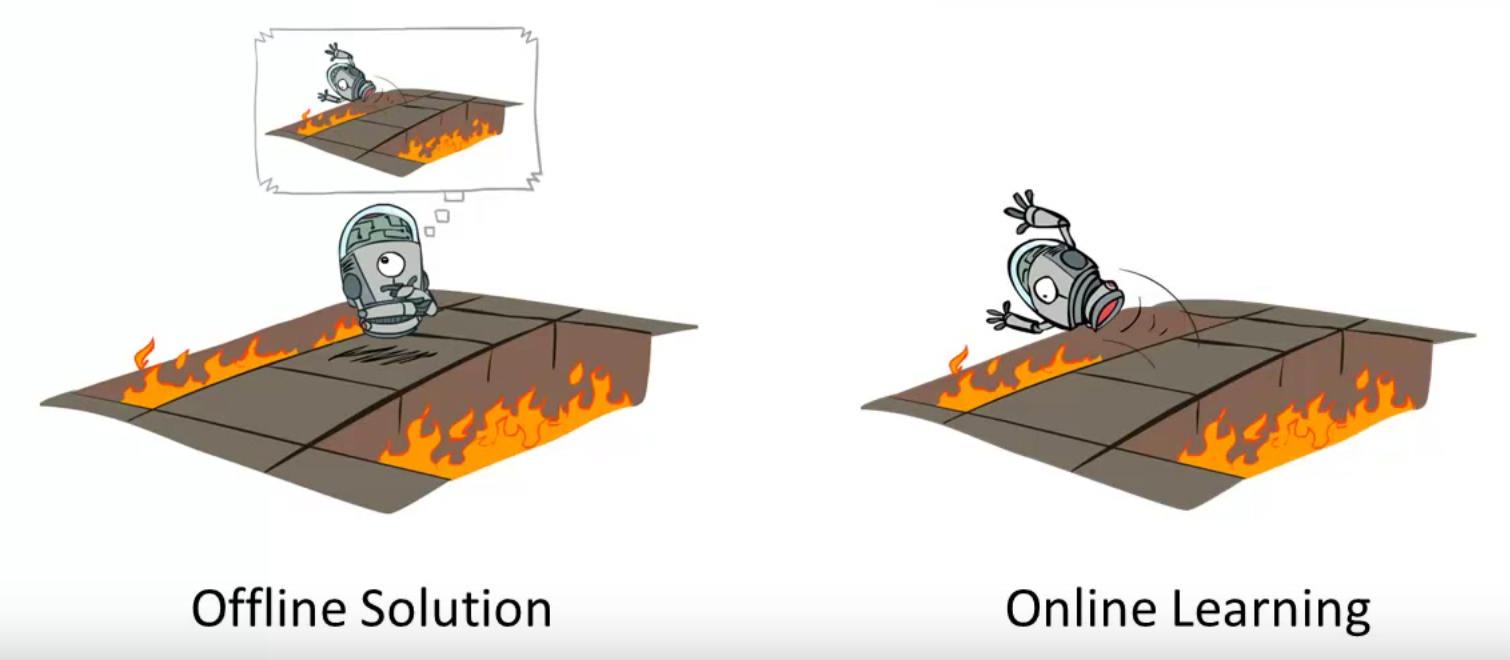
\includegraphics[width=0.785\linewidth,trim=0 50 0 0,clip]{Figures/rll4} 
\end{center}
\begin{enumerate}
\item  \high{Planning}: given complete Markov decision problem as input, compute policy with optimal expected return
\item \high{Learning}: Only have access to experience in the MDP, learn a near-optimal strategy
\end{enumerate}
We will focus on learning, but discuss planning along the way
\end{frame}

\begin{frame}\frametitle{Exploration vs. Exploitation}\small
\begin{itemize}
\item If we knew how the world works (embodied in $P$), then the policy should be deterministic 
\begin{itemize}
\onslide<2->\item  just select optimal action in each state
\end{itemize}
\onslide<3->\item Reinforcement learning is like trial-and-error learning
\onslide<4->\item The agent should discover a good policy from its experiences of the environment
\onslide<4->\item Without losing too much reward along the way

\onslide<5->\item Since we do not have complete knowledge of the world, taking what appears to be the optimal action may prevent us from finding better states/actions
\onslide<6->\item Interesting trade-off: 
\begin{itemize}
\item immediate reward (\high{exploitation}) vs. gaining knowledge that might enable higher future reward (\high{exploration})
\end{itemize}
\end{itemize}
\end{frame}

\begin{frame}\frametitle{Examples}\small
\begin{itemize}
\item Restaurant Selection
\begin{itemize}
\item \high{Exploitation}: Go to your favourite restaurant
\item \high{Exploration}: Try a new restaurant
\end{itemize}
\item Online Banner Advertisements
\begin{itemize}
\item \high{Exploitation}: Show the most successful advert
\item \high{Exploration}: Show a different advert
\end{itemize}
\item Oil Drilling
\begin{itemize}
\item \high{Exploitation}: Drill at the best known location
\item \high{Exploration}: Drill at a new location
\end{itemize}
\item Game Playing
\begin{itemize}
\item \high{Exploitation}: Play the move you believe is best
\item \high{Exploration}: Play an experimental move
\end{itemize}
\end{itemize}
\vspace{1mm}
\scriptsize [Slide credit: D. Silver]
\end{frame}



\begin{frame}\frametitle{Value function}\small
\begin{itemize}
\item The value function $V^\pi(s)$ assigns each state the expected reward 
\[
V^\pi(s)=\underset{a_{t},a_{t+i},s_{t+i}}{\mathbb{E}}\left[\sum_{i=1}^\infty\gamma^{i} r_{t+i} |s_t=s\right]
\]
\onslide<2->\item Usually not informative enough to make decisions.
\onslide<3->\item The $Q$-value $Q^{\pi}(s,a)$ is the expected reward of taking action $a$ in state $s$ and then continuing according to $\pi$.
\[
Q^\pi(s,a)=\underset{a_{t+i},s_{t+i}}{\mathbb{E}}\left[\sum_{i=1}^\infty\gamma^{i} r_{t+i} |s_t=s,a_t=a\right]
\]
\end{itemize}
\end{frame}

\begin{frame}\frametitle{Bellman equations}\small
\begin{itemize}
	\item The foundation of many RL algorithms
	{\footnotesize
	\begin{align*}\footnotesize
	V^\pi(s)&=\underset{a_{t},a_{t+i},s_{t+i}}{\mathbb{E}}\left[\sum_{i=1}^\infty\gamma^{i} r_{t+i} |s_t=s\right] \\
	&=\underset{a_{t}}{\mathbb{E}}\left[r_{t+1} |s_t=s\right]  +\gamma \underset{a_{t},a_{t+i},s_{t+i}}{\mathbb{E}}\left[\sum_{i=1}^\infty\gamma^{i} r_{t+i+1} |s_t=s\right] \\
	& = \underset{a_{t}}{\mathbb{E}}\left[r_{t+1} |s_t=s\right] +\gamma \underset{s_{t+1}}{\mathbb{E}}\left[V^{\pi}(s_{t+1})|s_t=s\right] \\
	& = \sum_{a,r}P^{\pi}(a|s_t)p(r|a,s_t)\cdot r+\gamma \sum_{a,s'}P^{\pi}(a|s_t)p(s'|a,s_t)\cdot V^{\pi}(s')
	\end{align*}}
	\item Similar equation holds for $Q$
		{\footnotesize
		\begin{align*}\footnotesize
		&Q^\pi(s,a)=\underset{a_{t+i},s_{t+i}}{\mathbb{E}}\left[\sum_{i=1}^\infty\gamma^{i} r_{t+i} |s_t=s,a_t=a\right] \\
		& = \sum_{r}p(r|a,s_t)\cdot r+ \gamma\sum_{s'}p(s'|a,s_t)\cdot V^{\pi}(s') \\
		&=\sum_{r}p(r|a,s_t)\cdot r+ \gamma\sum_{a',s'}p(s'|a,s_t)p(a'|s')\cdot Q^{\pi}(s',a')
		\end{align*}}
\end{itemize}
\end{frame}

\begin{frame}\frametitle{Solving Bellman equations}\small
\begin{itemize}
	\item The Bellman equations are a set of linear equations with a unique solution.
	\onslide<2->\item Can solve fast(er) because the linear mapping is a contractive mapping.
	\onslide<3->\item This lets you know the quality of each state/action under your policy - \high{policy evaluation}.
	\onslide<4->\item You can improve by picking $\pi'(s)=\max_a Q^{\pi}(s,a)$ - \high{policy improvement}.
	\onslide<5->\item Can show the iterative policy evaluation and improvement converges to the optimal policy.
	\onslide<6->\item Are we done? \onslide<7-> Why isn't this enough?
	\onslide<8->
	\begin{itemize}
		\item Need to know the model! Usually isn't known.
		\item Number of states is usually huge (how many unique states does a chess game have?) 
	\end{itemize}
\end{itemize}
\end{frame}

\begin{frame}\frametitle{Optimal Bellman equations}\small
\begin{itemize}
	\item First step is understand the Bellman equation for the optimal policy $\pi^*$
	\onslide<2->\item Under this policy $V^*(s)=\max_a Q^*(s,a)$
		{\footnotesize
		\begin{align*}\footnotesize
		V^*(s)& = \max_a\left[\mathbb{E}\left[r_{t+1} |s_t=s,a_t=a\right] +\gamma \underset{s_{t+1}}{\mathbb{E}}\left[V^{*}(s_{t+1})|s_t=s,a_t=a\right]\right] \\
		&= \max_a\left[\sum_{r}p(r|a,s_t)\cdot r+\gamma \sum_{s'}p(s'|a,s_t)\cdot V^*(s')\right] \\
		Q^*(s,a)&=\mathbb{E}\left[r_{t+1} |s_t=s,a_t=a\right]+ \gamma\underset{s_{t+1}}{\mathbb{E}}\left[\max_{a'}Q^{*}(s_{t+1},a')|s_t=s,a_t=a\right] \\
		&= \sum_{r}p(r|a,s_t)\cdot r+\gamma \sum_{s'}p(s'|a,s_t)\cdot\max_{a'} Q^*(s',a')
		\end{align*}}
	\onslide<3-> \item Set on nonlinear equations.
	\onslide<4-> \item Same issues as before.
	
\end{itemize}
\end{frame}


\begin{frame}\frametitle{Q-learning intuition}\small
\begin{itemize}
	\item Q-learning is a simple algorithm to find the optimal policy without knowing the model.
		\onslide<2->\item $Q^*$ is the unique solution to the optimal Bellman equation.
	\[
	Q^*(s,a)=\mathbb{E}\left[r_{t+1} |s_t=s,a_t=a\right]+ \gamma\underset{s_{t+1}}{\mathbb{E}}\left[\max_{a'}Q^{*}(s_{t+1},a')|s_t=s,a_t=a\right]
	\]
	\onslide<3->\item We don't know the model and don't want to update all states simultaneously.
	\onslide<4->\item Solution - given sample $s_t,a_t,r_{t+1},s_{t+1}$ from the environment update your $Q$-values so they are closer to satisfying the bellman equation.
	\begin{itemize}
		\item \high{off-policy} method: Samples don't have to be from the optimal policy.

	\end{itemize} 
	\item Samples need to be diverse enough to see everything - exploration.
\end{itemize}
\end{frame}

\begin{frame}\frametitle{Exploration vs exploitation}\small
\begin{itemize}
	\item Given $Q$-value the best thing we can do (given our limited knowledge) is to take $a=\arg\max_{a'}Q(s,a')$ - \high{exploitation}
	\onslide<2->\item How do we balance exploration with exploitation?
	\onslide<3->\item Simplest solution: $\epsilon$-greedy. 
	\begin{itemize}
		\item With probability $1-\epsilon$ pick $a=\arg\max_{a'}Q(s,a')$ (i.e. greedy)
		\item With probability $\epsilon$ pick any other action uniformly.
	\end{itemize} 
	\onslide<4->\item Another idea - softmax using $Q$ values
	\begin{itemize}
		\item With probability $1-\epsilon$ pick $a=\arg\max_{a'}Q(s,a')$ (i.e. greedy)
		\item With probability $\epsilon$ pick any other action with probability $\propto\exp(\beta Q(s,a))$.
	\end{itemize} 
	\onslide<5->\item Other fancier solutions exist, many leading methods use simple $\epsilon$-greedy sampling.
	
\end{itemize}
\end{frame}


\begin{frame}\frametitle{Q-learning algorithm}\small
\vspace{-0.5cm}
\begin{figure}
	 \includegraphics[width=0.9\linewidth]{Figures/Qalgo}
 \end{figure}
\vspace{-0.5cm}
\begin{itemize}
	\onslide<2->\item Can prove convergence to the optimal $Q^*$ under mild conditions.
	\onslide<3->\item Update is equivalent to gradient descent on loss $||R+\gamma\max_a Q(S',a)-Q(s,a)||^2$.
	\item At optimal Q, the loss is 0.
	% \onslide<4->\item Why $L_2$ loss? Optimal solution is the mean which is what we are looking for!
	
\end{itemize}
\end{frame}

\begin{frame}\frametitle{Bootstrapping}\small

\begin{itemize}
	\item Another way to think about Q-learning.
	\item $Q(s,a)$ is the expected reward, can use Monte-Carlo estimation.
	\onslide<2->\item Problem - you update only after the episode ends, can be very long (or infinite).
	\onslide<3->\item Q-learning solution - take only 1 step forward and estimate the future using our Q value - \high{bootstrapping}.
	\begin{itemize}
		\item "learn a guess from a guess"
	\end{itemize} 
	\onslide<4->\item Q-learning is just one algorithm in a family of algorithms that use this idea.
\end{itemize}
\end{frame}

\begin{frame}\frametitle{Function approximation}\small

\begin{itemize}
	\item Q-learning still scales badly with large state spaces, how many states does a chess game have? Need to save the full table!
	\onslide<2->\item Similar states, e.g. move all chess pieces two steps to the left, at treated as totally different.
	\onslide<3->\item Solution: Instead of $Q$ being a $S\times A$ table it is a parametrized function.
	\onslide<4-> \item Looking for function $\hat{Q}(s,a;\bw)\approx Q^*(s,a)$
	\begin{itemize}
		\onslide<5->\item Linear functions $Q(s,a;\bw)=\bw^T\phi(s,a)$.
		\item Neural network
	\end{itemize}
	\onslide<5->\item Hopefully can generalize to unseen states.
	\onslide<6->\item Problem: Each change to parameters changes all states/actions - can lead to instability.
	\onslide<7->\item For non-linear Q-learning can diverge.
	
\end{itemize}
\end{frame}


\begin{frame}\frametitle{Deep Q-learning}\small

\begin{itemize}
	\item We have a function approximator $Q(s,a;\theta)$, standard is neural net but doesn't have to be.
	\onslide<2->\item What is the objective that we are optimizing?
	\onslide<3->\item  We want to minimize $\mathbb{E}_{\rho}[||R+\gamma\max_{a'} Q(S',a')-Q(s,a)||^2]$
	\begin{itemize}
		\item $\rho$ is a distribution over states, depends on $\theta$!
	\end{itemize}
	\onslide<4->\item Two terms depend on $Q$, don't want to take gradients w.r. to $\gamma\max_aQ(S',a)$
	\onslide<5->\item We want to correct our previous estimation given the new information.
			\vspace{-0.2cm}
	\begin{figure}
		\includegraphics[width=0.85\linewidth]{Figures/Qalgo2}
		\vspace{-0.4cm}
		\caption{Take from:rll.berkeley.edu/deeprlcourse}
	\end{figure}
		\vspace{-0.5cm}
	\onslide<5->\item This simple approach doesn't work well as is.
	
	
\end{itemize}
\end{frame}

\begin{frame}\frametitle{Issues and solutions}\small

\begin{itemize}
	\item \high{Problem}: data in the minibatch is highly correlated
	\begin{itemize}
		\item Consecutive samples are from the same eposide and probably similar states.
		\item Solution: \high{Replay memory}.
		\item You store a large memory buffer of previous $(s,a,r,s')$ (notice this is all you need for Q-learning) and sample from it to get diverse minibatch.
	\end{itemize}
	\item \high{Problem}: The data distribution keeps changing
\begin{itemize}
	\item Since we aren't optimizing $y_i$ its like solving a different (but related) least squares each iteration.
	\item We can stabilize by fixing a \high{target network} for a few iterations 
\end{itemize}

\end{itemize}

	\begin{figure}
	\includegraphics[width=0.75\linewidth]{Figures/DQN}
	\vspace{-0.4cm}
	\caption{Take from:rll.berkeley.edu/deeprlcourse}
\end{figure}
\end{frame}

\begin{frame}\frametitle{Example: DQN on atari}\small

\begin{itemize}
	\item Trained a NN from scratch on atari games 

\begin{figure}
	\includegraphics[width=0.75\linewidth]{Figures/DQN_arc}
\end{figure}
\onslide<2->\item Ablation study
\begin{figure}
	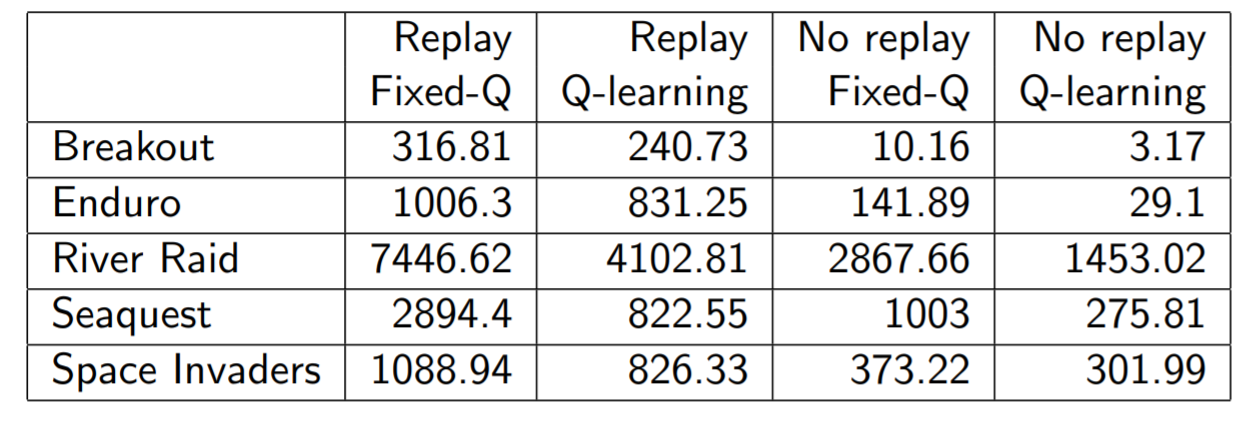
\includegraphics[width=0.75\linewidth]{Figures/ablation}
\end{figure}
\end{itemize}

\end{frame}


\begin{frame}\frametitle{RL recap}\small

\begin{itemize}
	\item Learning from experience not from labeled examples.
	\onslide<2->\item Why is RL hard?
	\begin{itemize}
		\onslide<3->\item Limited feedback.
		\onslide<4->\item Delayed rewards.
		\onslide<5->\item Your model effect what you
		 see.
		\onslide<6->\item Huge state space.
	\end{itemize}
	\onslide<7-> \item Usually solved by learning the value function or optimizing the policy (not covered)
	% \onslide<8-> \item Model based method but less successful at the moment.
	\onslide<9-> \item How do you define the rewards? Can be tricky.
	\begin{itemize}
		\item Bad rewards can lead to \high{reward hacking}
	\end{itemize}
	
\end{itemize}

\end{frame}

\begin{frame}\frametitle{Q-Learning recap}\small

\begin{itemize}
	\item Try to find $Q$ that satisfies the optimal Bellman conditions
	\onslide<2->\item \high{Off-policy} algorithm - Doesn't have to follow a greedy policy to evaluate it.
	\onslide<3->\item \high{Model free} algorithm - Doesn't have any model for instantaneous reward or dynamics.
	\onslide<4->\item Learns a seperate value for each $s,a$ pair - doesn't scale up to huge state spaces.
	\onslide<5->\item Can scale using a function approximation
	\begin{itemize}
		\item No more theoretical guarantees.
		\item Can diverge. 
		\item Some simple tricks help a lot.
	\end{itemize}
	
	
\end{itemize}

\end{frame}



%
%%%%%%%%%%%%%%%%%%%%%%%%%%%%%%%%%%%%%%%%%%%%% 
%%%%%%%%%%%%%%%%%%%%%%%%%%%%%%%%%%%%%%%%%%%%% 
%
%% PREVIOUS VERSION %
%
%%%%%%%%%%%%%%%%%%%%%%%%%%%%%%%%%%%%%%%%%%%%% 
%%%%%%%%%%%%%%%%%%%%%%%%%%%%%%%%%%%%%%%%%%%%% 
%
%\section{Introduction}
%
%
%
%\begin{frame}\frametitle{Today}\small
%\begin{itemize}
%\item Learn to play games
%\item Reinforcement Learning
%\end{itemize}
%\vspace{2mm}
%
%% \begin{figure}
%% 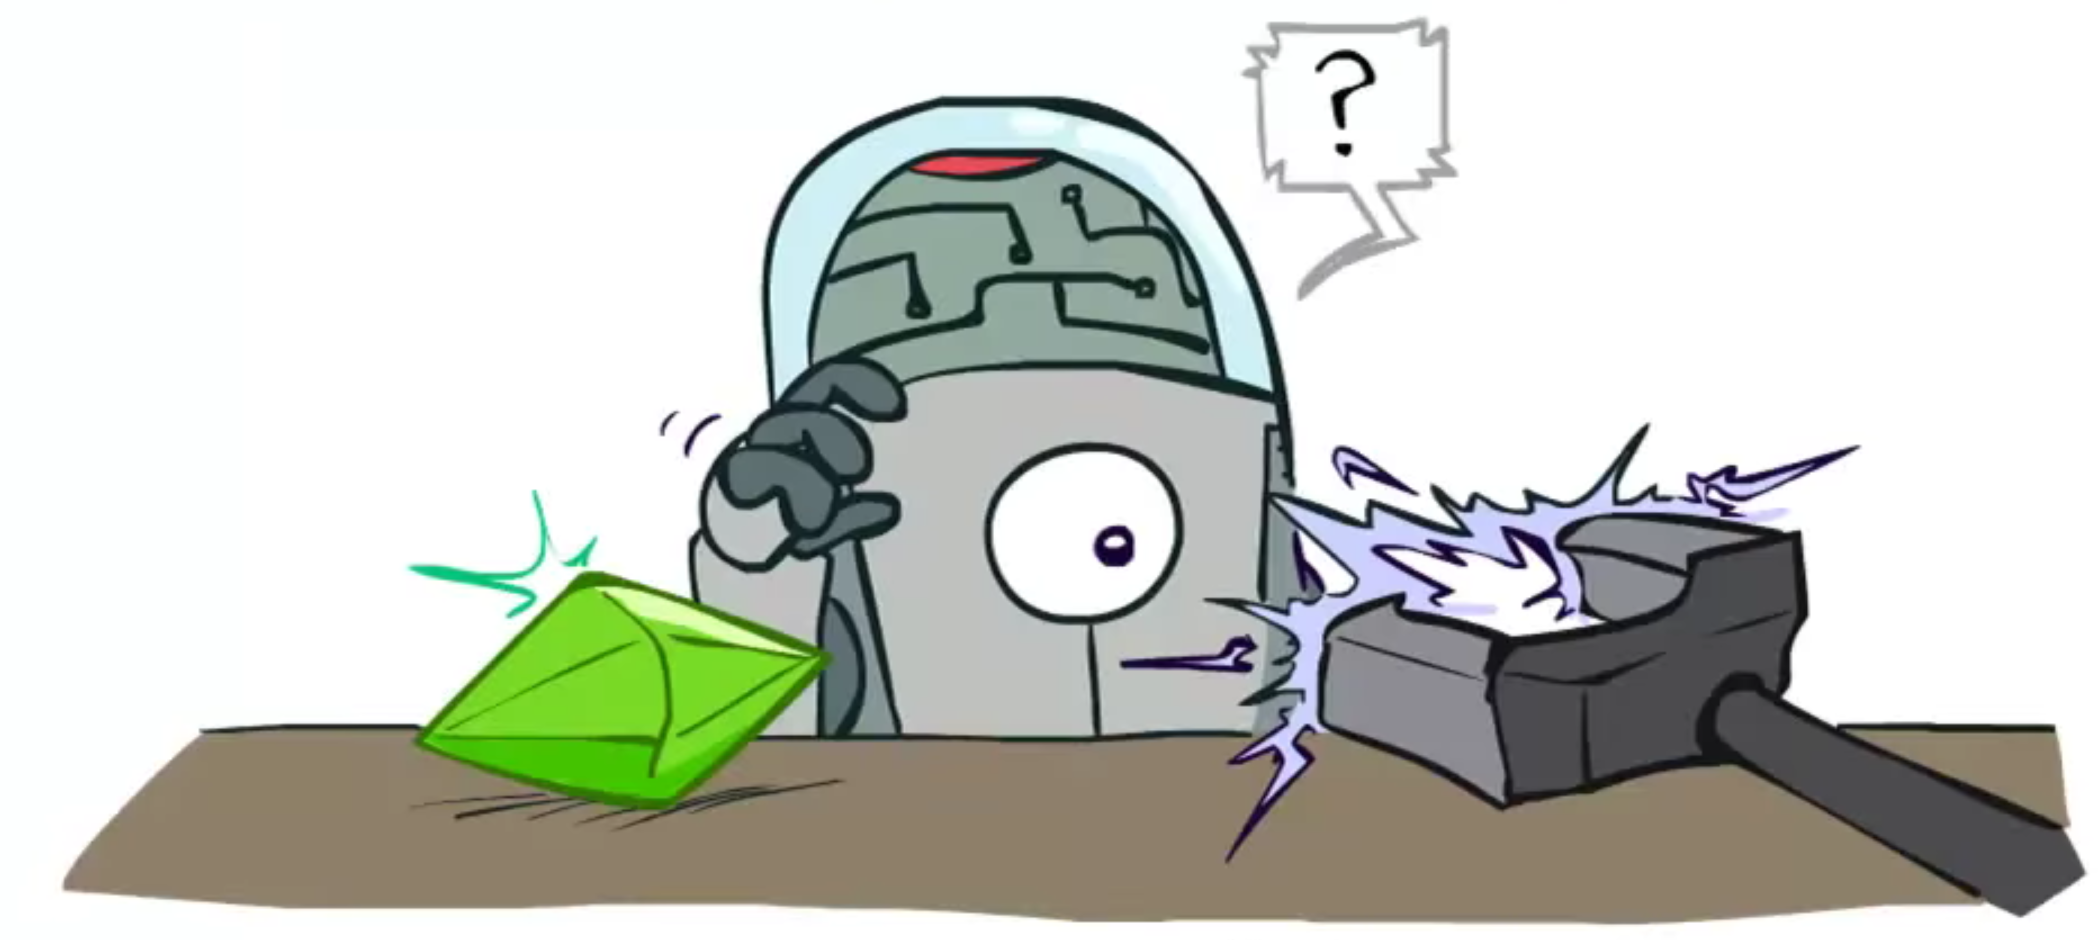
\includegraphics[width =0.78\linewidth]{../old_course_material/slides/figs/lecture19/rll1}
%% \end{figure}
%% \vspace{2mm}
%% 
%% \scriptsize [pic from: Peter Abbeel]
%\end{frame}
%
%\begin{frame}\frametitle{Playing Games: Atari}\small
%\begin{figure}
%\href{run:videos/intro/deep_mind.mp4}{
%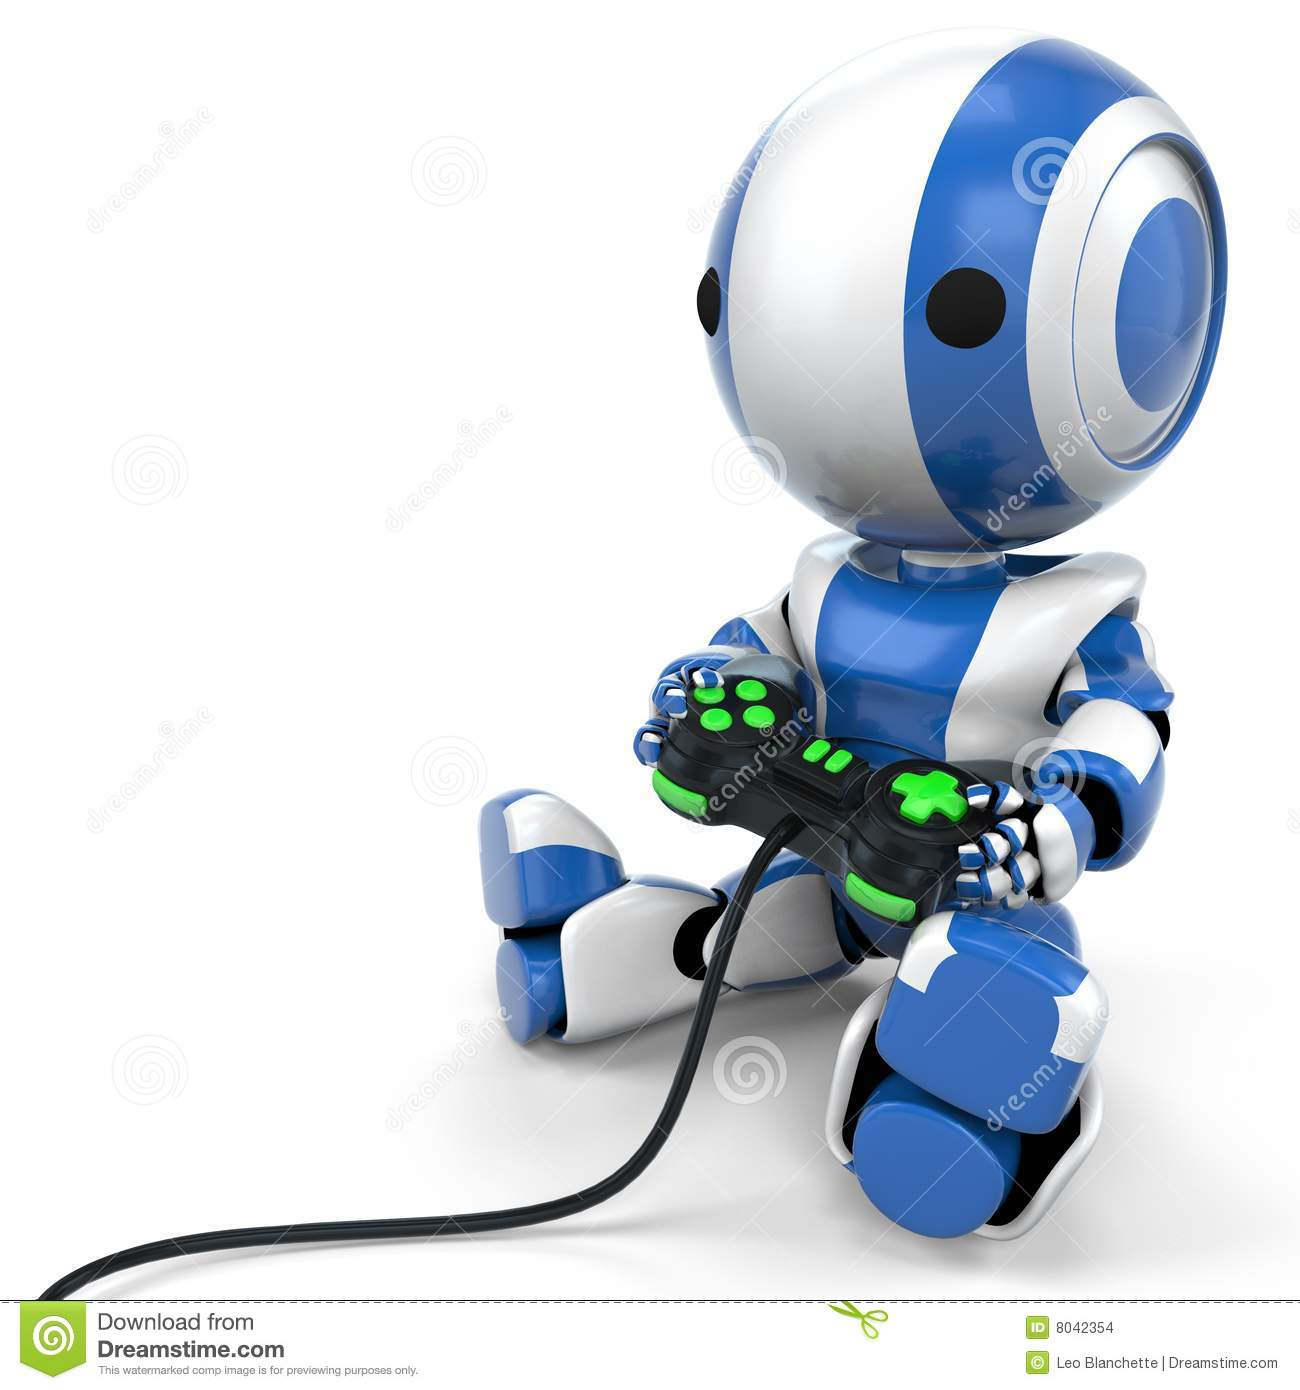
\includegraphics[width =0.6\linewidth,trim=0 69 0 0,clip]{Figures/robot_game.jpg}\\
%{\color{magenta}{\url{https://www.youtube.com/watch?v=V1eYniJ0Rnk}}}
%}
%\end{figure}
%\end{frame}
%
%\begin{frame}\frametitle{Playing Games: Super Mario}\small
%\begin{figure}
%\href{run:videos/intro/super_mario.mp4}{
%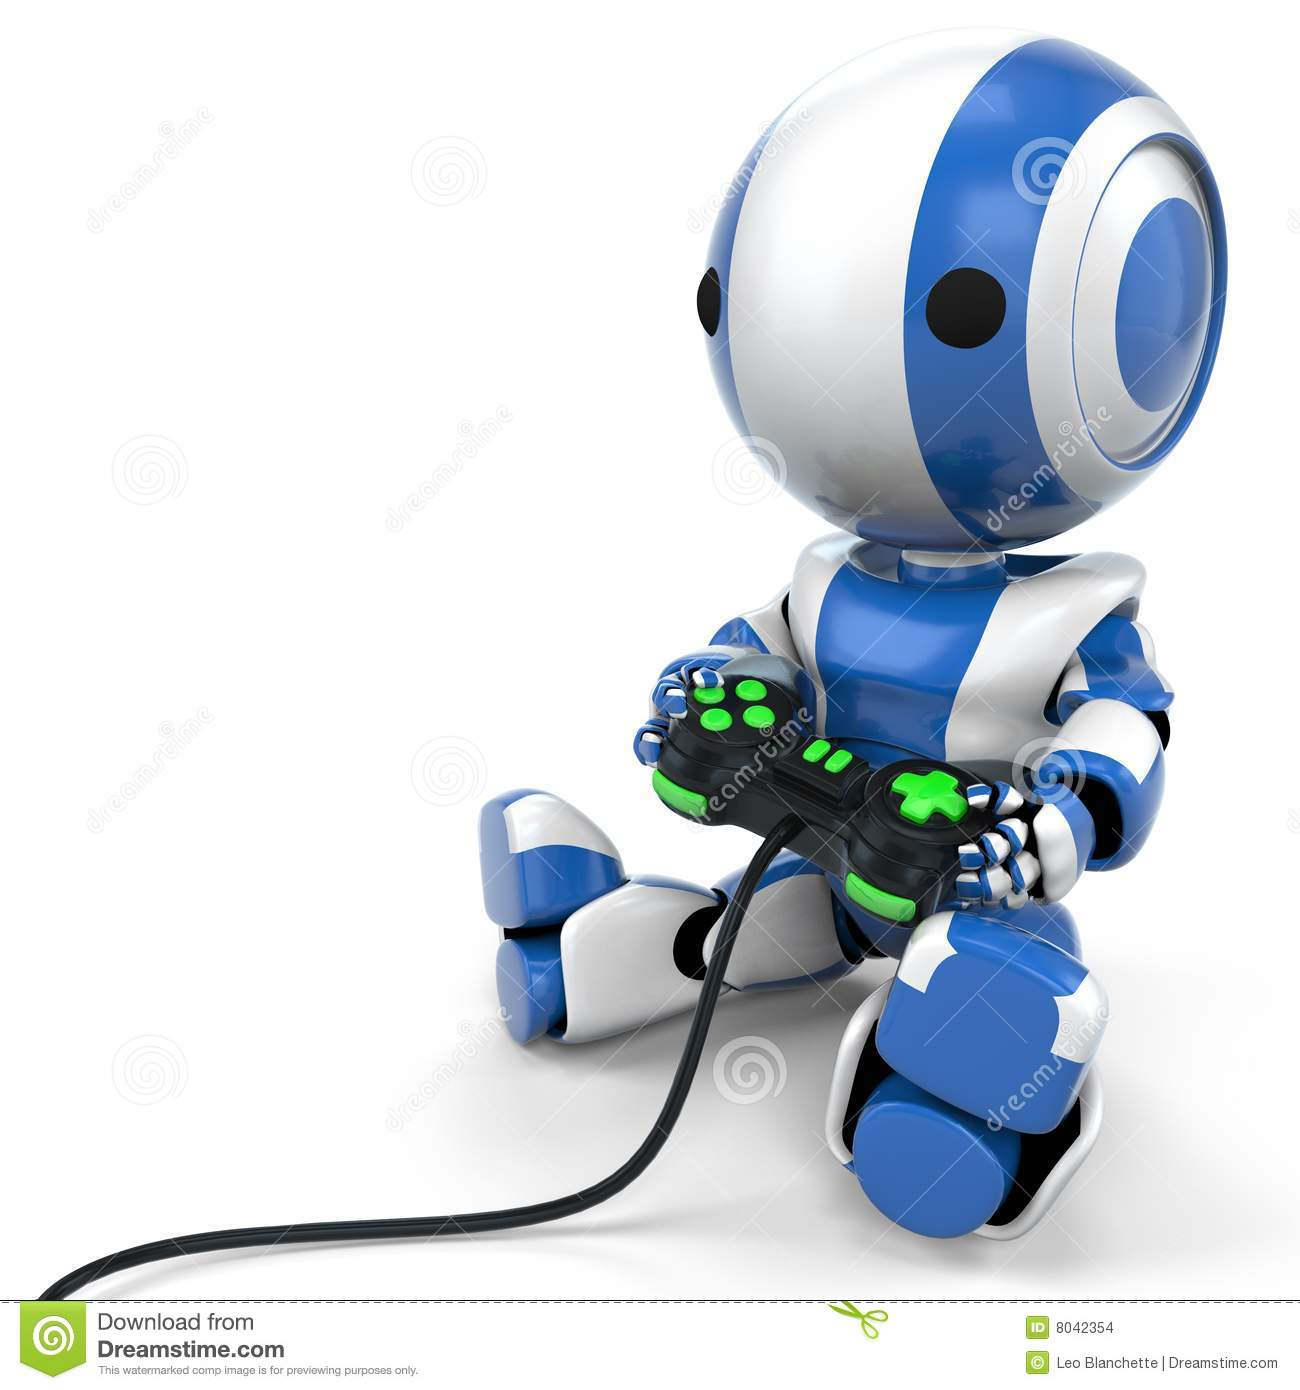
\includegraphics[width =0.6\linewidth,trim=0 69 0 0,clip]{Figures/robot_game.jpg}\\
%{\color{magenta}{\url{https://www.youtube.com/watch?v=wfL4L_l4U9A}}}
%}
%\end{figure}
%\end{frame}
%
%\begin{frame}\frametitle{Making Pancakes!}\small
%\begin{figure}
%\href{run:videos/lecture19/pancakes.mp4}{
%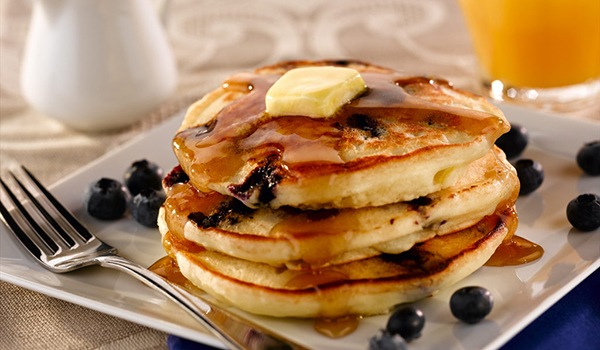
\includegraphics[width=0.9\linewidth]{Figures/pancakes1}\\
%{\color{magenta}{\url{https://www.youtube.com/watch?v=W_gxLKSsSIE}}}
%}
%\end{figure}
%\end{frame}
%
%
%\begin{frame}\frametitle{Reinforcement Learning Resources}\small
%\begin{itemize}
%
%\item {\it Reinforcement Learning: An Introduction second edition}, Sutton \& Barto Book (2016)
%\item  \href{https://www.youtube.com/watch?v=2pWv7GOvuf0}{Video lectures by David Silver}
%\end{itemize}
%\end{frame}
%
%% \begin{frame}\frametitle{What is Reinforcement Learning?}\small
%% \begin{figure}
%% 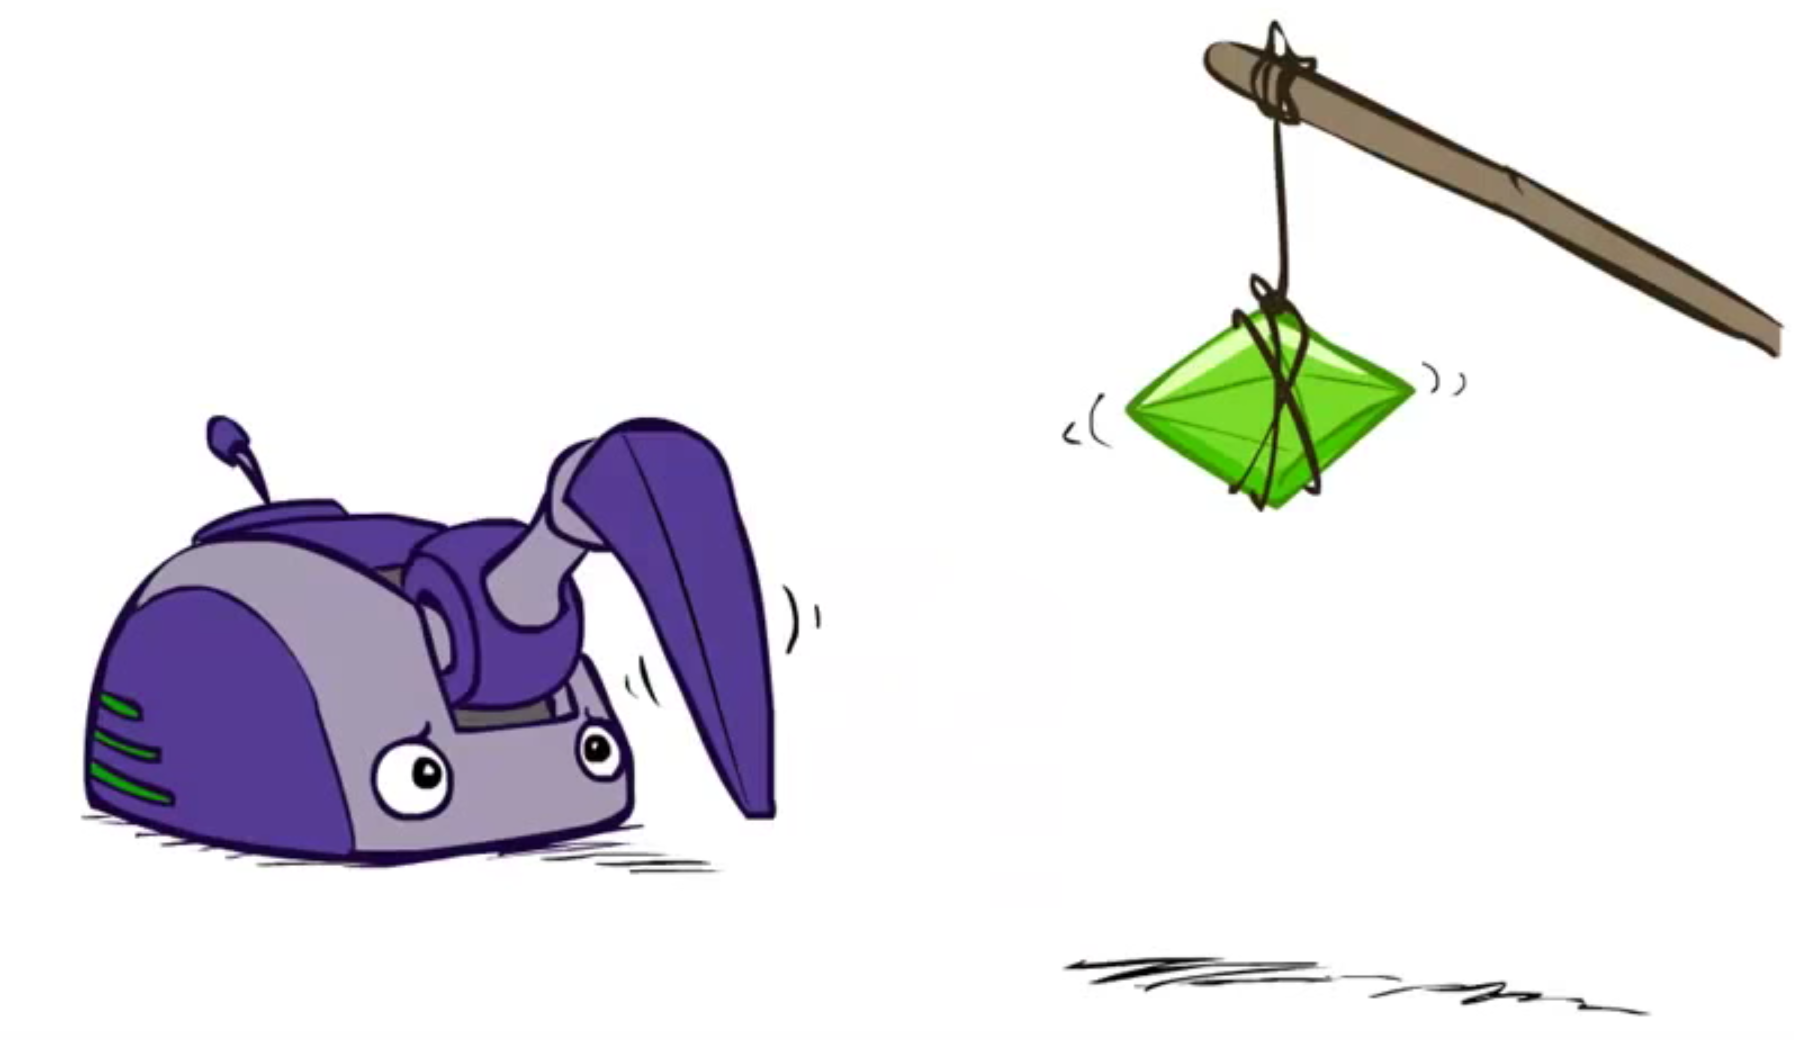
\includegraphics[width=0.9\linewidth]{../old_course_material/slides/figs/lecture19/rll2}
%% \end{figure}
%% \vspace{5mm}
%% \scriptsize [pic from: Peter Abbeel]
%% \end{frame}
%% 
%
%\begin{frame}\frametitle{Reinforcement Learning}\small
%\begin{itemize}
%\item Learning algorithms differ in the information available to learner
%\begin{itemize}
%\onslide<2->\item \high{Supervised}: correct outputs
%\onslide<3->\item \high{Unsupervised}: no feedback, must construct measure of good output
%\onslide<4->\item \high{Reinforcement learning}: Reward.
%\end{itemize}
%\onslide<5->\item More realistic learning scenario: 
%\begin{itemize}
%\item Continuous stream of input information, and actions\\[0.7mm] 
%\onslide<6->\item Effects of action depend on state of the world\\[0.7mm] 
%\onslide<7->\item Obtain reward that depends on world state and actions\\[0.7mm] 
%\begin{itemize}
%\onslide<8->\item You know the reward for your action, not other actions.
%\onslide<9->\item Could be a delay between action and reward.
%\end{itemize}
%\end{itemize}
%\end{itemize}
%\end{frame}
%
%\begin{frame}\frametitle{Reinforcement Learning}\small
%\vspace{8mm}
%
%\begin{figure}
%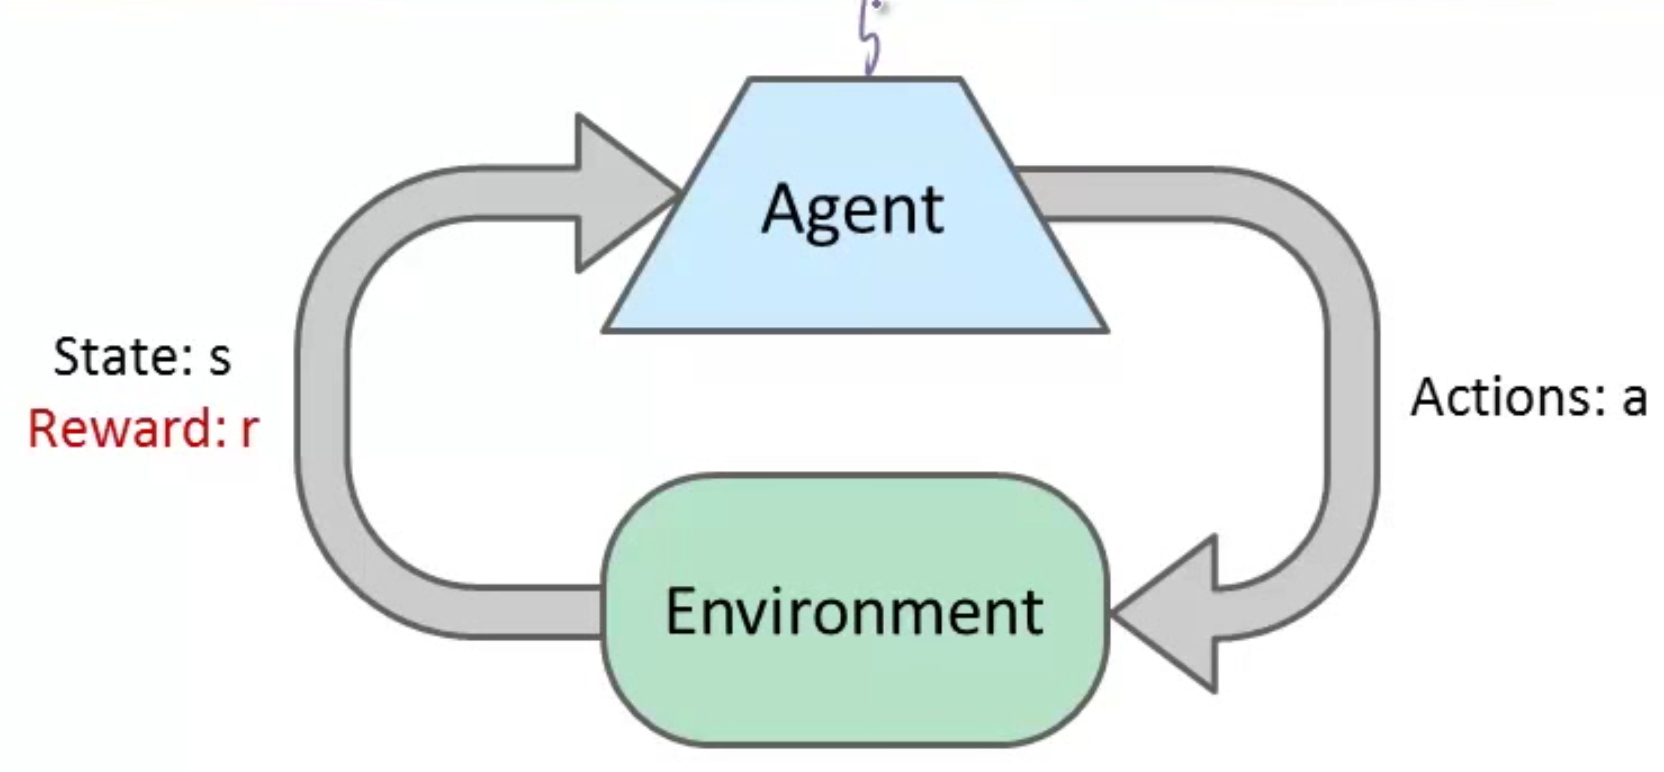
\includegraphics[width=0.85\linewidth]{Figures/rll3}
%\end{figure}
%\vspace{7mm}
%
%\scriptsize [pic from: Peter Abbeel]
%\end{frame}
%
%\begin{frame}\frametitle{Example: Tic Tac Toe, Notation}\small
%\vspace{4mm}
%\begin{figure}
%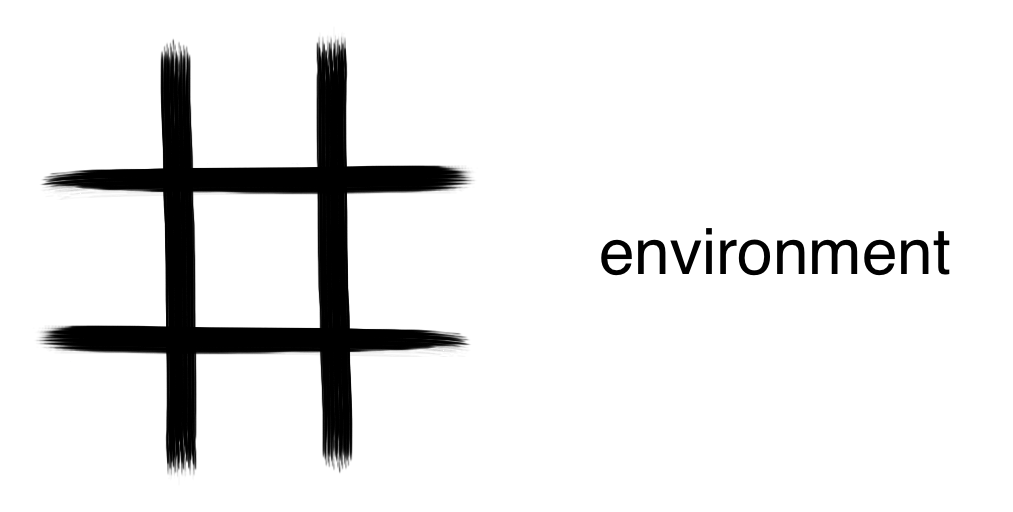
\includegraphics[width=0.75\linewidth]{Figures/tic1d}
%\end{figure}
%\vspace{5mm}
%\end{frame}
%
%\begin{frame}\frametitle{Example: Tic Tac Toe, Notation}\small
%\vspace{4mm}
%
%\begin{figure}
%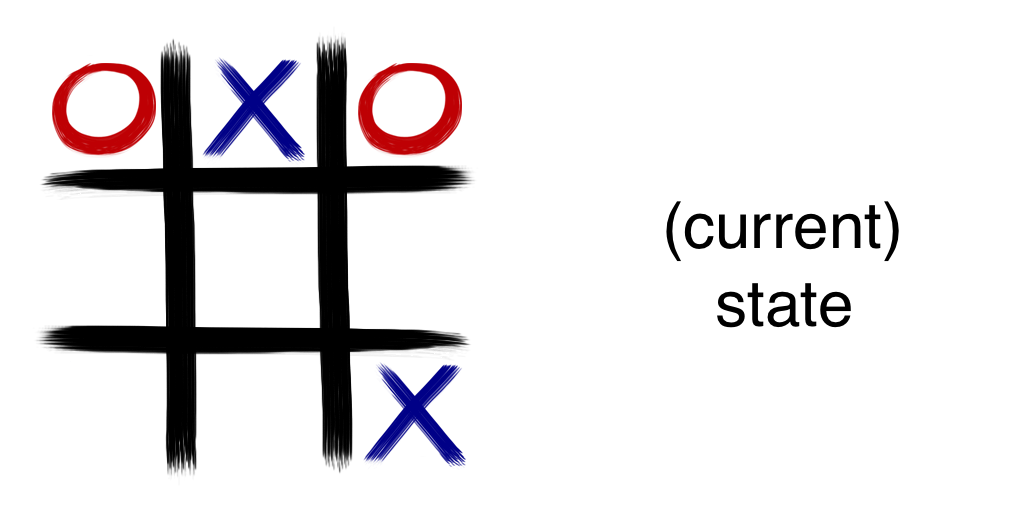
\includegraphics[width=0.75\linewidth]{Figures/tic1c}
%\end{figure}
%\vspace{5mm}
%\end{frame}
%
%\begin{frame}\frametitle{Example: Tic Tac Toe, Notation}\small
%\vspace{4mm}
%
%\begin{figure}
%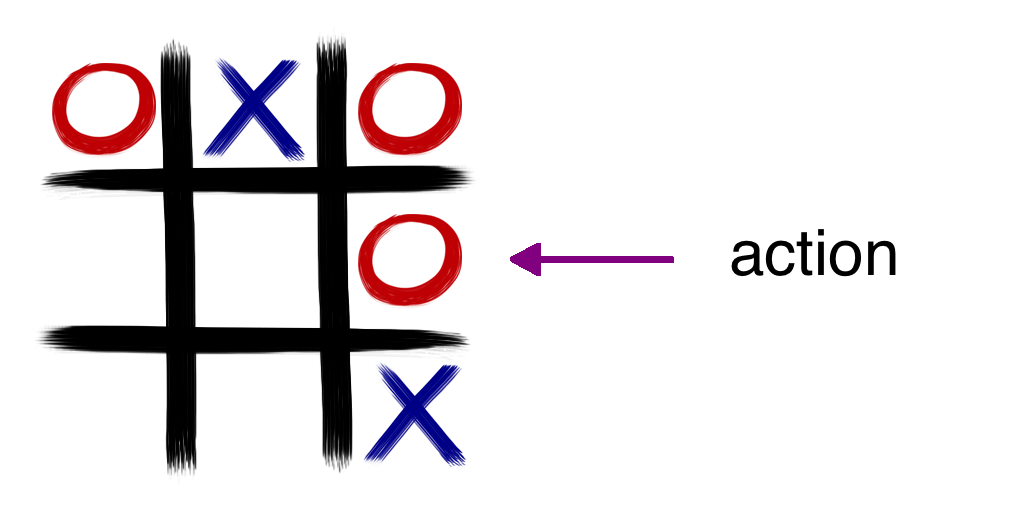
\includegraphics[width=0.75\linewidth]{Figures/tic1b}
%\end{figure}
%\vspace{5mm}
%\end{frame}
%
%\begin{frame}\frametitle{Example: Tic Tac Toe, Notation}\small
%\vspace{4mm}
%
%\begin{figure}
%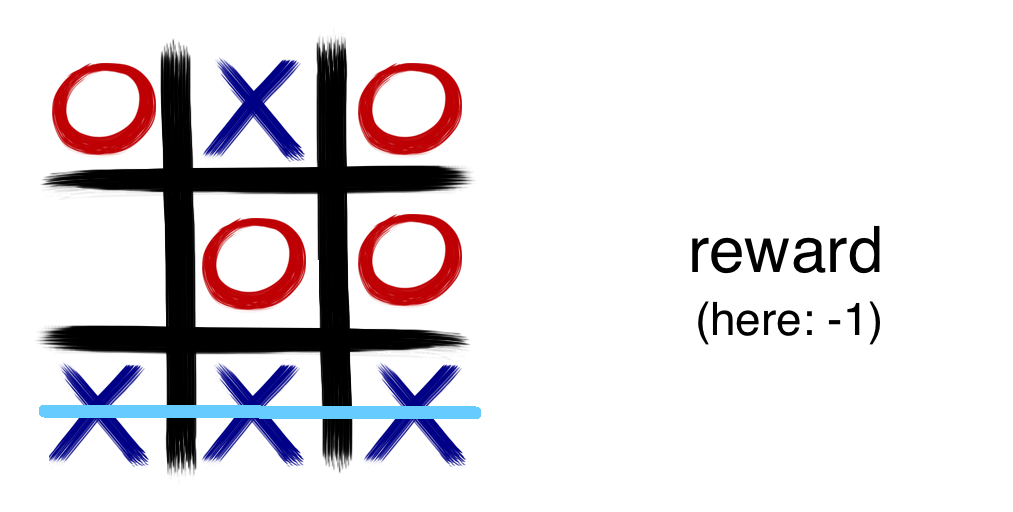
\includegraphics[width=0.75\linewidth]{Figures/tic1e}
%\end{figure}
%\vspace{5mm}
%\end{frame}
%
%\iffalse
%\begin{frame}\frametitle{Formulating Reinforcement Learning}\small
%\begin{itemize}
%\item World described by a discrete, finite set of states and actions
%\onslide<2->\item At every time step t, we are in a \high{state} $s_t$, and we:
%\begin{itemize}
%\onslide<3->\item Take an \high{action} $a_t$ (possibly null action)
%\onslide<4->\item Receive some \high{reward} $r_{t+1}$
%\onslide<5->\item Move into a new state $s_{t+1}$
%\end{itemize}
%\onslide<6->\item Decisions can be described by a \high{policy} $\pi$
%\begin{itemize}
%\onslide<7->\item  a selection of which action to take, based on the current state: $a_t=\pi(s_t)$
%\end{itemize}
%\onslide<8->\item Aim is to \high{maximize the total reward} we receive over time:
%\[
%r_{t}+r_{t+1}+r_{t+2}+\dots
%\]
%\vspace{-4mm}
%\onslide<9->\item Sometimes a future reward is discounted by $\gamma^{k-1}$, where $k$ is the number of time-steps in the future when it is received:
%\[
%r_{t}+\gamma r_{t+1}+\gamma^2 r_{t+2}+\dots
%\]
%\end{itemize}
%\end{frame}
%\fi
%
%\begin{frame}\frametitle{Formulating Reinforcement Learning}\small
%\begin{itemize}
%\item World described by a  set of states and actions
%\onslide<2->\item At every time step t, we are in a \high{state} $s_t$, and we:
%\begin{itemize}
%\onslide<3->\item Take an \high{action} $a_t$ (possibly null action)
%\onslide<4->\item Receive some \high{reward} $r_{t+1}$
%\onslide<5->\item Move into a new state $s_{t+1}$
%\end{itemize}
%\onslide<6->\item An RL agent may include one or more of these components:
%\begin{itemize}
%\item \high{Policy} $\pi$: agent's behaviour function
%\onslide<7->\item \high{Value function}: how good is each state and/or action
%\onslide<8->\item \high{Model}: agent's representation of the environment
%\end{itemize}
%\end{itemize}
%\end{frame}
%
%\begin{frame}\frametitle{Policy}\small
%\begin{itemize}
%\item A \high{policy} is the agent's behaviour.
%\item It's a selection of which action to take, based on the current state
%\item Deterministic policy: $a = \pi(s)$
%\item Stochastic policy: $\pi(a|s) = P[a_t = a|s_t = s]$
%\end{itemize}
%
%\vspace{30mm}
%\scriptsize [Slide credit: D. Silver]
%\end{frame}
%
%\begin{frame}\frametitle{Value Function}\small
%\begin{itemize}
%\item \high{Value function} is the expected future reward
%\item Used to evaluate the goodness/badness of states
%\onslide<2-> \item Our aim will be to maximize the value function (the total reward we receive over time): find the policy with the highest expected reward
%%\item And therefore to select between actions, e.g.
%\onslide<3-> \item By following a policy $\pi$, the value function is defined as:
%\begin{eqnarray}
%V^{\pi}(s_t) &=& \mathbb{E}[r_t + \gamma r_{t+1} + \gamma^2 r_{t+2} + \cdots] \nonumber
%\end{eqnarray}
%\item $\gamma$ is called a \high{discount rate}, and it is always $0\leq\gamma\leq 1$
%\onslide<4->\item If $\gamma$ close to $1$, rewards further in the future count more, and we say that the agent is ``farsighted''
%\item $\gamma$ is less than $1$ because there is usually a time limit to the sequence of actions needed to solve a task (we prefer rewards sooner rather than later)
%\end{itemize}
%
%\vspace{10mm}
%\scriptsize [Slide credit: D. Silver]
%\end{frame}
%
%
%\begin{frame}\frametitle{Model}\small
%\begin{itemize}
%\item The model describes the \high{environment} by a distribution over rewards and state transitions:
%\[
%P(s_{t+1}=s', r_{t+1}=r' | s_t = s, a_t = a)
%\]
%%\item The world and the actor may not be deterministic, or our model of the world may be incomplete
%\item We assume the \high{Markov property}: the future depends on the past only through the current state
%%\onslide<3->\item We describe the \high{environment} by a distribution over rewards and state transitions:
%%\[
%%P(s_{t+1}=s', r_{t+1}=r' | s_t = s, a_t = a)
%%\]
%%\onslide<4->\item The \high{policy} can also be non-deterministic:
%%\[
%%P(a_t = a | s_t = s)
%%\]
%%\onslide<5->\item Policy is not a fixed sequence of actions, but instead a conditional plan
%\end{itemize}
%\begin{figure}
%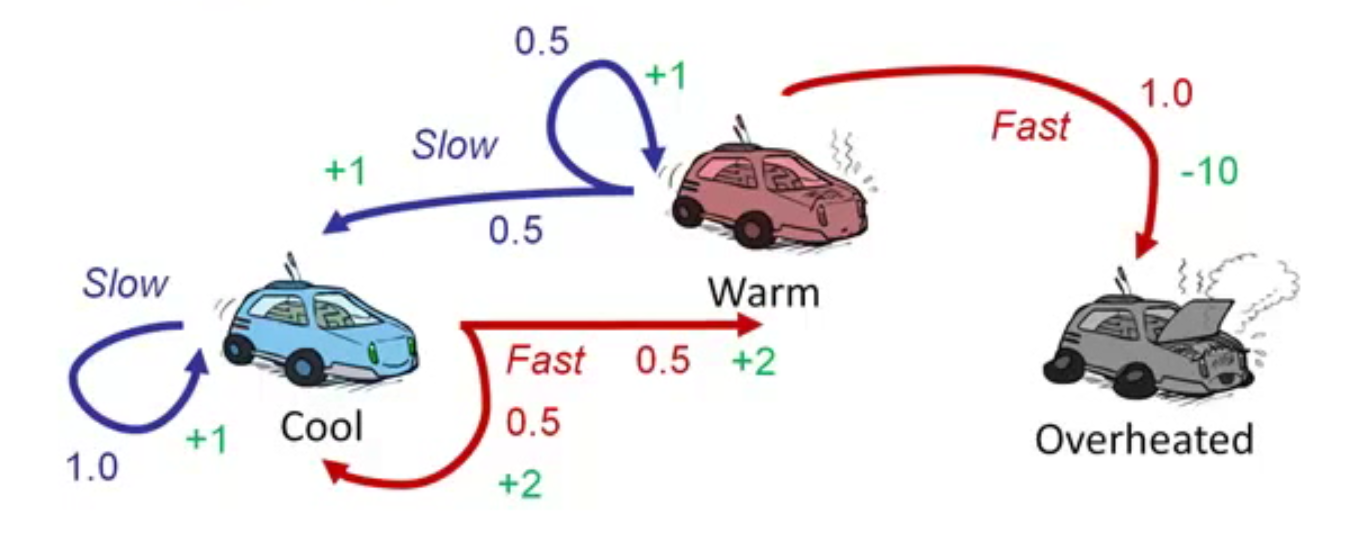
\includegraphics[width=0.7\linewidth]{Figures/rll6} 
%\end{figure}
%\end{frame}
%
%
%\begin{frame}\frametitle{Maze Example}\small
%\begin{figure}
%\begin{minipage}{0.5\linewidth}
%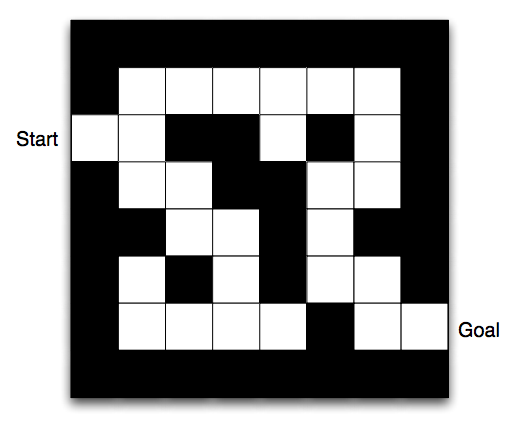
\includegraphics[width=\linewidth]{Figures/maze1}
%\end{minipage}
%\hspace{3mm}
%\begin{minipage}{0.45\linewidth}
%\begin{itemize}
%\item Rewards: \onslide<2-> $-1$ per time-step
%\item Actions: \onslide<3-> N, E, S, W
%\item States: \onslide<4-> Agent's location
%\end{itemize}
%\end{minipage}
%\end{figure}
%
%\vspace{12mm}
%\scriptsize [Slide credit: D. Silver]
%\end{frame}
%
%\begin{frame}\frametitle{Maze Example}\small
%\begin{figure}
%\begin{minipage}{0.5\linewidth}
%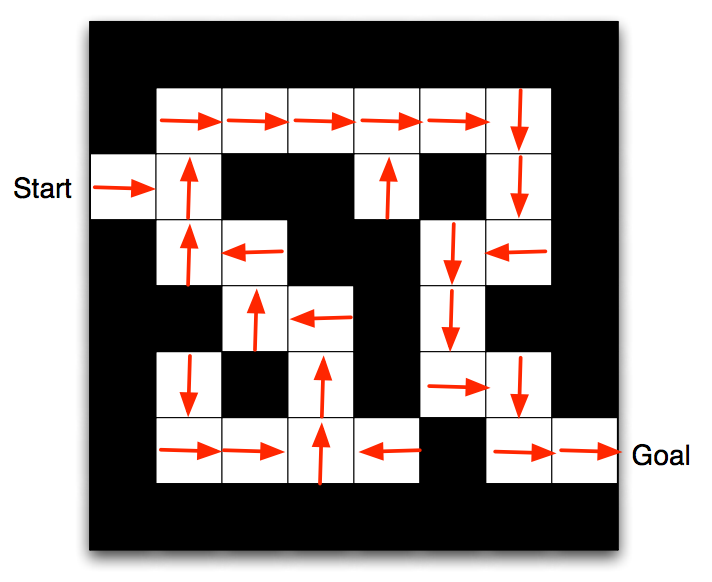
\includegraphics[width=\linewidth]{Figures/maze2}
%\end{minipage}
%\hspace{3mm}
%\begin{minipage}{0.45\linewidth}
%\begin{itemize}
%\item Arrows represent policy $\pi(s)$ for each state $s$
%\end{itemize}
%\end{minipage}
%\end{figure}
%
%\vspace{14mm}
%\scriptsize [Slide credit: D. Silver]
%\end{frame}
%
%\begin{frame}\frametitle{Maze Example}\small
%\begin{figure}
%\begin{minipage}{0.5\linewidth}
%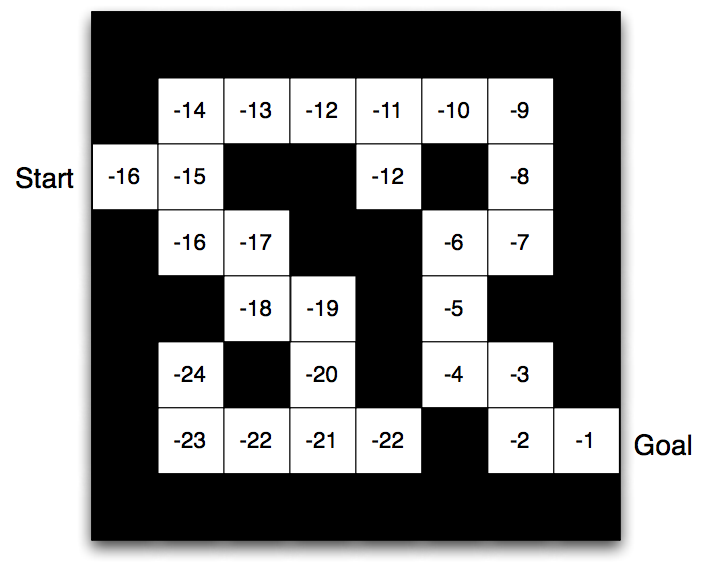
\includegraphics[width=\linewidth]{Figures/maze3}
%\end{minipage}
%\hspace{3mm}
%\begin{minipage}{0.45\linewidth}
%\begin{itemize}
%\item Numbers represent value $V^{\pi}(s)$ of each state $s$
%\end{itemize}
%\end{minipage}
%\end{figure}
%
%\vspace{14mm}
%\scriptsize [Slide credit: D. Silver]
%\end{frame}
%
%
%\iffalse
%\begin{frame}\frametitle{Formulating Reinforcement Learning}\small
%\begin{itemize}
%\item (from previous slide) Sometimes a future reward is discounted by $\gamma^{k-1}$, where $k$ is the number of time-steps in the future when it is received
%\item $\gamma$ is called a \high{discount rate}, and it is always $0\leq\gamma\leq 1$
%\onslide<2->\item If $\gamma$ close to $1$, rewards further in the future count more, and we say that the agent is ``farsighted''
%\onslide<3->\item $\gamma$ is less than $1$ because there is usually a time limit to the sequence of actions needed to solve a task (we prefer rewards sooner rather than later)
%\end{itemize}
%\end{frame}
%\fi
%
%\begin{frame}\frametitle{Example: Tic-Tac-Toe}\small
%\begin{itemize}
%\item Consider the game tic-tac-toe:
%\begin{itemize}
%\onslide<2->\item \high{reward}: \onslide<3-> win/lose/tie the game $(+1/-1/0)$ [only at final move in given game]
%\onslide<4->\item \high{state}: \onslide<5->positions of X's and O's on the board
%\onslide<6->\item \high{policy}: mapping from states to actions 
%\begin{itemize}
%\onslide<7->\item based on rules of game: choice of one open position
%\end{itemize}
%\onslide<8->\item \high{value function}: prediction of reward in future, based    on current state
%\end{itemize}
%\onslide<9->\item In tic-tac-toe, since state space is tractable, can use a table to represent value function 
%\end{itemize}
%\end{frame}
%
%\begin{frame}\frametitle{RL \& Tic-Tac-Toe}\small
%%\vspace{-0.3cm}
%\begin{itemize}
%\item Each board position (taking into account symmetry) has some probability
%\end{itemize}
%\begin{minipage}{4cm}
%\begin{center}
%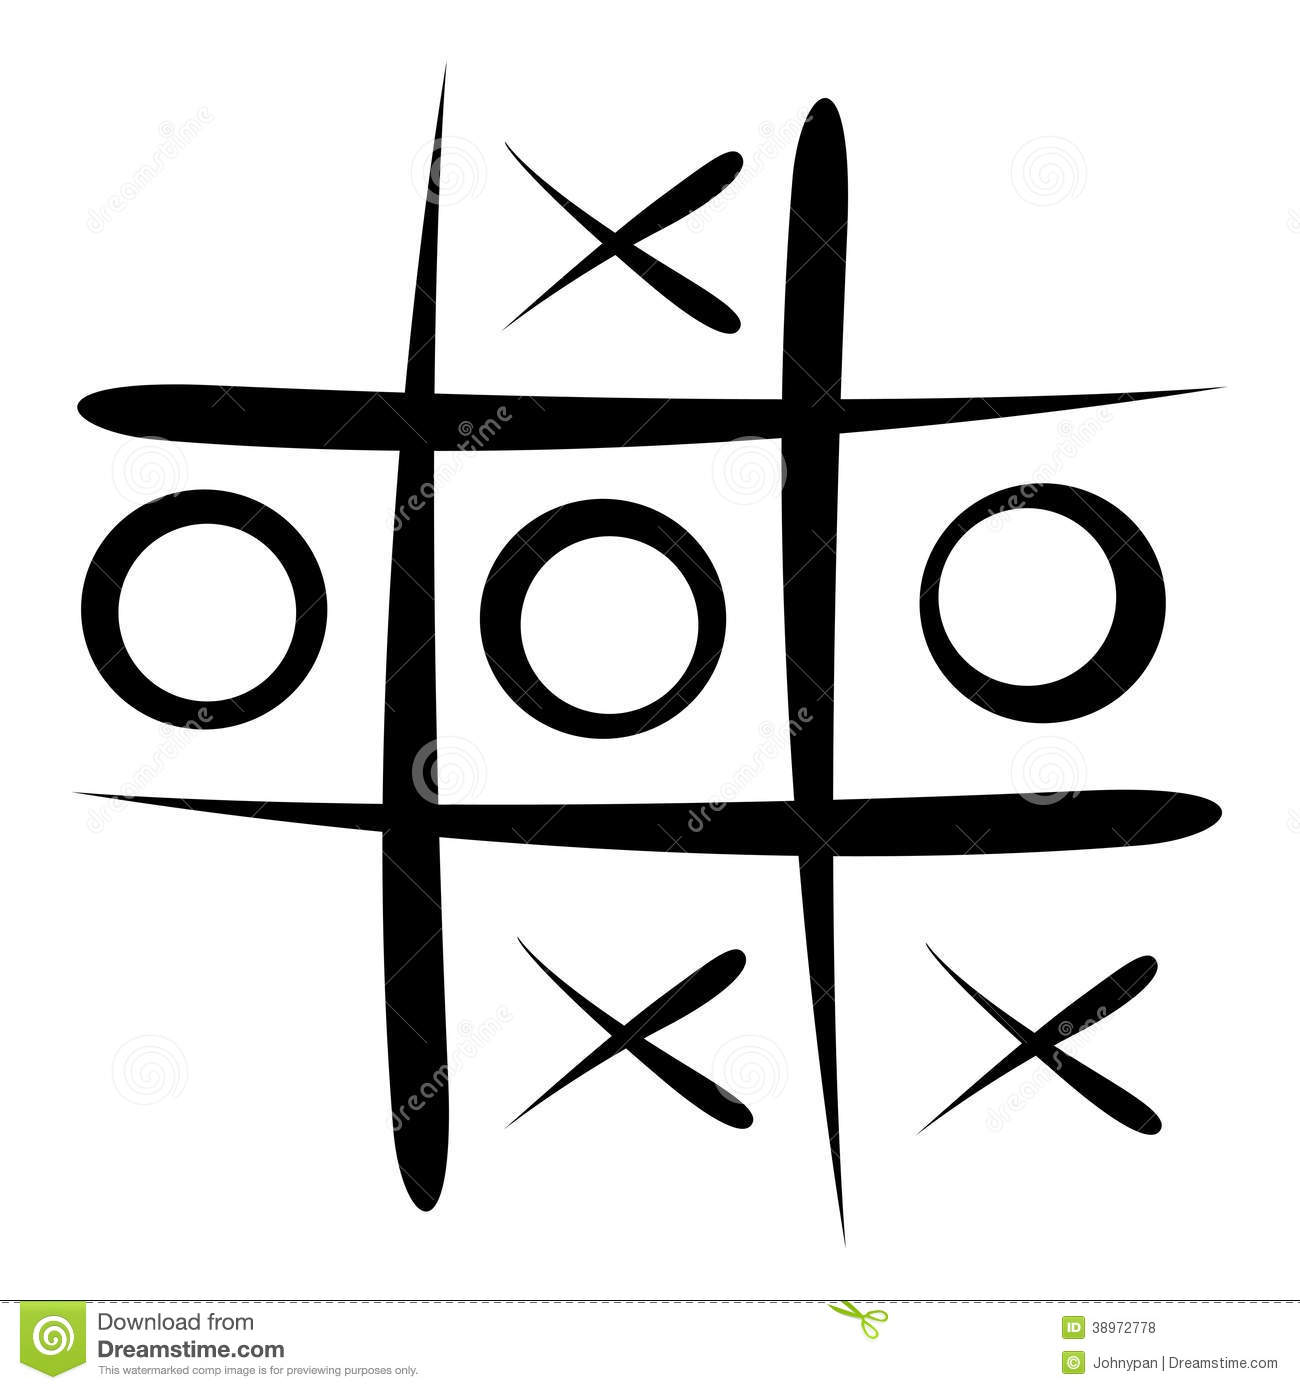
\includegraphics[width=1.0\linewidth]{Figures/tictac} 
%\end{center}
%\end{minipage}
%\begin{minipage}{7cm}
%\begin{itemize}
%%\item Each board position (taking into account symmetry) has some probability
%\onslide<2->\item Simple learning process: 
%\begin{itemize}
%\onslide<3->\item start with all values = 0.5
%\onslide<4->\item \high{policy}: choose move with highest probability of winning given current legal moves from current state
%\onslide<5->\item update entries in table based on outcome of each game
%\onslide<6->\item After many games value function will represent true probability of winning from each state
%\end{itemize}
%%\item Can try alternative policy: sometimes select moves randomly (exploration)
%\end{itemize}
%\end{minipage}
%\begin{itemize}
%\onslide<7->\item Can try alternative policy: sometimes select moves randomly (exploration)
%\end{itemize}
%\end{frame}
%
%\iffalse
%\begin{frame}\frametitle{Acting Under Uncertainty}\small
%\begin{itemize}
%\item The world and the actor may not be deterministic, or our model of the world may be incomplete
%\onslide<2->\item We assume the \high{Markov property}: the future depends on the past only through the current state
%\onslide<3->\item We describe the \high{environment} by a distribution over rewards and state transitions:
%\[
%P(s_{t+1}=s', r_{t+1}=r' | s_t = s, a_t = a)
%\]
%\onslide<4->\item The \high{policy} can also be non-deterministic:
%\[
%P(a_t = a | s_t = s)
%\]
%\onslide<5->\item Policy is not a fixed sequence of actions, but instead a conditional plan
%\end{itemize}
%\end{frame}
%\fi
%
%\begin{frame}\frametitle{MDP}\small
%\begin{itemize}
%\item Markov Decision Problem (MDP): tuple $(S,A,P,\gamma)$ where $P$ is
%\[
%P(s_{t+1}=s', r_{t+1}=r' | s_t = s, a_t = a)
%\]
%\onslide<2->\item Main assumption: Markovian dynamics and reward.
%\onslide<3->\item Standard MDP problems:
%\begin{enumerate}
%\onslide<4->\item  \high{Planning}: given complete Markov decision problem as input, compute policy with optimal expected return
%\begin{figure}
%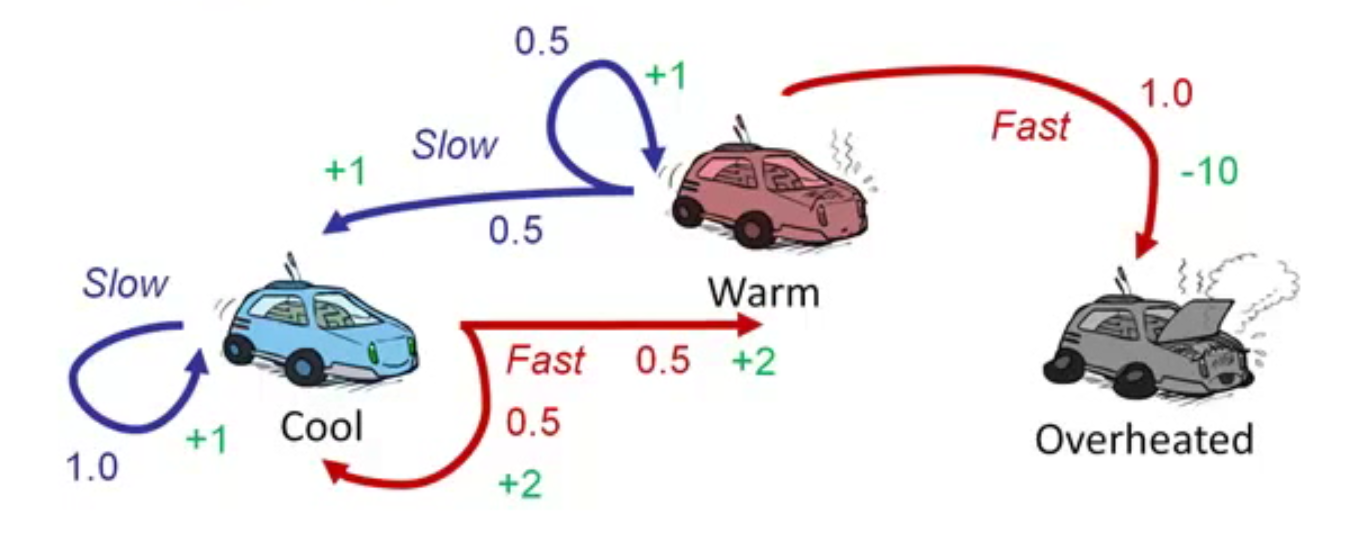
\includegraphics[width=0.7\linewidth]{Figures/rll6} 
%\end{figure}
%\end{enumerate}
%\end{itemize}
%\scriptsize [Pic: P. Abbeel]
%\end{frame}
%
%
%\begin{frame}\frametitle{Basic Problems}\small
%\begin{itemize}
%\item Markov Decision Problem (MDP): tuple $(S,A,P,\gamma)$ where $P$ is
%\[
%P(s_{t+1}=s', r_{t+1}=r' | s_t = s, a_t = a)
%\]
%\item Standard MDP problems:
%\begin{enumerate}
%\item  \high{Planning}: given complete Markov decision problem as input, compute policy with optimal expected return\\[1mm]
%\item \high{Learning}: We don't know which states are good or what the actions do. We must try out the actions and states to learn what to do
%\end{enumerate}
%\end{itemize}
%\vspace{28mm}
%
%\scriptsize [P. Abbeel]
%\end{frame}
%
%\begin{frame}\frametitle{Example of Standard MDP Problem}\small
%\begin{center}
%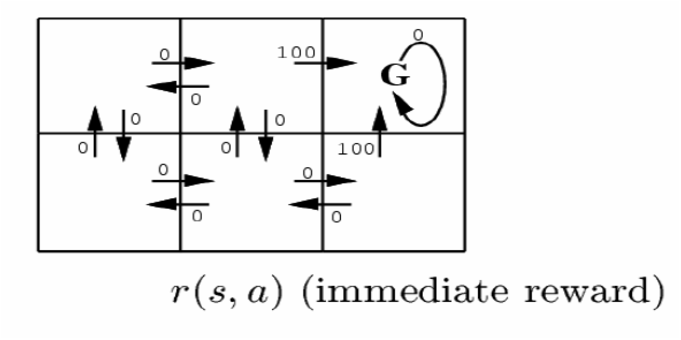
\includegraphics[width=0.54\linewidth]{Figures/tic_tac_rl} 
%\end{center}
%\begin{enumerate}
%\item  \high{Planning}: given complete Markov decision problem as input, compute policy with optimal expected return
%\item \high{Learning}: Only have access to experience in the MDP, learn a near-optimal strategy
%\end{enumerate}
%%We will focus on learning, but discuss planning along the way
%\end{frame}
%
%\begin{frame}\frametitle{Example of Standard MDP Problem}\small
%\begin{center}
%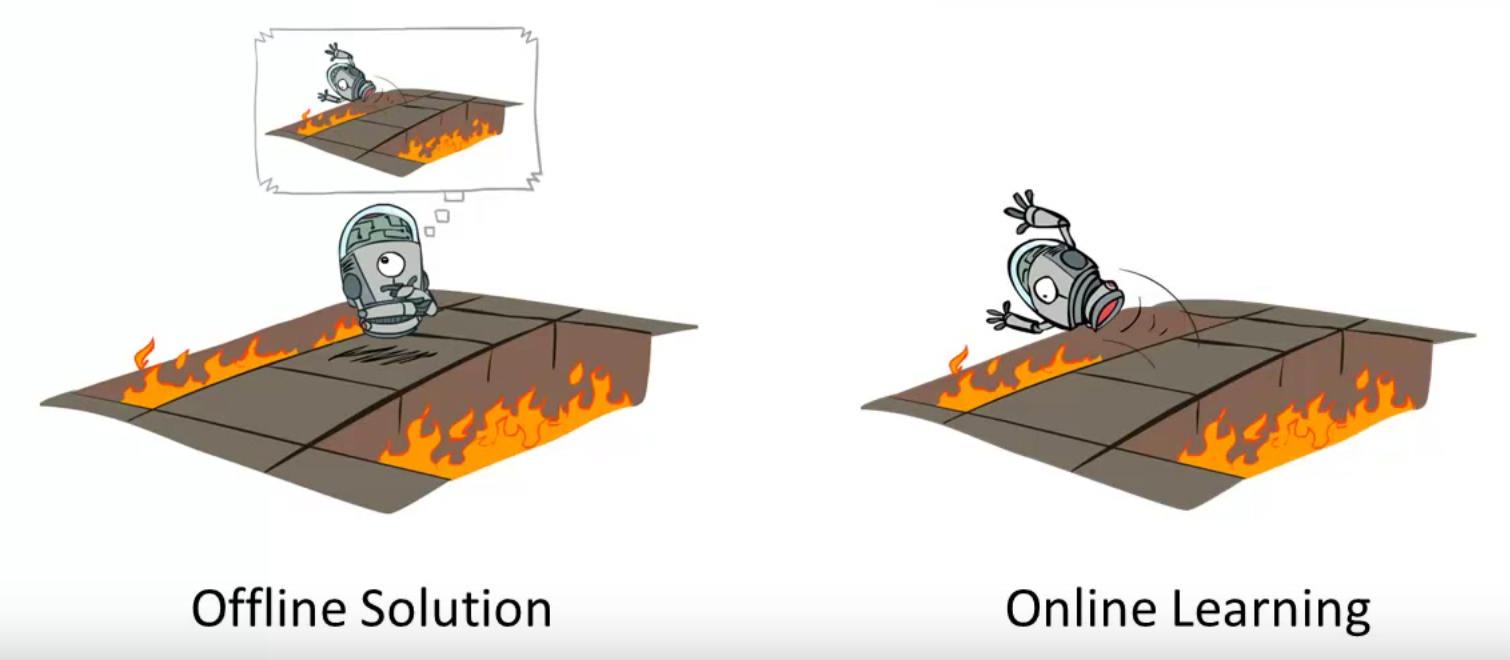
\includegraphics[width=0.785\linewidth,trim=0 50 0 0,clip]{Figures/rll4} 
%\end{center}
%\begin{enumerate}
%\item  \high{Planning}: given complete Markov decision problem as input, compute policy with optimal expected return
%\item \high{Learning}: Only have access to experience in the MDP, learn a near-optimal strategy
%\end{enumerate}
%We will focus on learning, but discuss planning along the way
%\end{frame}
%
%\begin{frame}\frametitle{Exploration vs. Exploitation}\small
%\begin{itemize}
%\item If we knew how the world works (embodied in $P$), then the policy should be deterministic 
%\begin{itemize}
%\onslide<2->\item  just select optimal action in each state
%\end{itemize}
%\onslide<3->\item Reinforcement learning is like trial-and-error learning
%\onslide<4->\item The agent should discover a good policy from its experiences of the environment
%\onslide<4->\item Without losing too much reward along the way
%
%\onslide<5->\item Since we do not have complete knowledge of the world, taking what appears to be the optimal action may prevent us from finding better states/actions
%\onslide<6->\item Interesting trade-off: 
%\begin{itemize}
%\item immediate reward (\high{exploitation}) vs. gaining knowledge that might enable higher future reward (\high{exploration})
%\end{itemize}
%\end{itemize}
%\end{frame}
%
%\begin{frame}\frametitle{Examples}\small
%\begin{itemize}
%\item Restaurant Selection
%\begin{itemize}
%\item \high{Exploitation}: Go to your favourite restaurant
%\item \high{Exploration}: Try a new restaurant
%\end{itemize}
%\item Online Banner Advertisements
%\begin{itemize}
%\item \high{Exploitation}: Show the most successful advert
%\item \high{Exploration}: Show a different advert
%\end{itemize}
%\item Oil Drilling
%\begin{itemize}
%\item \high{Exploitation}: Drill at the best known location
%\item \high{Exploration}: Drill at a new location
%\end{itemize}
%\item Game Playing
%\begin{itemize}
%\item \high{Exploitation}: Play the move you believe is best
%\item \high{Exploration}: Play an experimental move
%\end{itemize}
%\end{itemize}
%\vspace{1mm}
%\scriptsize [Slide credit: D. Silver]
%\end{frame}
%
%\begin{frame}\frametitle{Value function}\small
%\begin{itemize}
%\item The value function $V^\pi(s)$ assigns each state the expected reward 
%\[
%V^\pi(s)=\underset{a_{t},a_{t+i},s_{t+i}}{\mathbb{E}}\left[\sum_{i=1}^\infty\gamma^{i} r_{t+i} |s_t=s\right]
%\]
%\onslide<2->\item Usually not informative enough to make decisions.
%\onslide<3->\item The $Q$-value $Q^{\pi}(s,a)$ is the expected reward of taking action $a$ in state $s$ and then continuing according to $\pi$.
%\[
%Q^\pi(s,a)=\underset{a_{t+i},s_{t+i}}{\mathbb{E}}\left[\sum_{i=1}^\infty\gamma^{i} r_{t+i} |s_t=s,a_t=a\right]
%\]
%\end{itemize}
%\end{frame}
%
%\begin{frame}\frametitle{Bellman equations}\small
%\begin{itemize}
%	\item The foundation of many RL algorithms
%	{\footnotesize
%	\begin{align*}\footnotesize
%	V^\pi(s)&=\underset{a_{t},a_{t+i},s_{t+i}}{\mathbb{E}}\left[\sum_{i=1}^\infty\gamma^{i} r_{t+i} |s_t=s\right] \\
%	&=\underset{a_{t}}{\mathbb{E}}\left[r_{t+1} |s_t=s\right]  +\gamma \underset{a_{t},a_{t+i},s_{t+i}}{\mathbb{E}}\left[\sum_{i=1}^\infty\gamma^{i} r_{t+i+1} |s_t=s\right] \\
%	& = \underset{a_{t}}{\mathbb{E}}\left[r_{t+1} |s_t=s\right] +\gamma \underset{s_{t+1}}{\mathbb{E}}\left[V^{\pi}(s_{t+1})|s_t=s\right] \\
%	& = \sum_{a,r}P^{\pi}(a|s_t)p(r|a,s_t)\cdot r+\gamma \sum_{a,s'}P^{\pi}(a|s_t)p(s'|a,s_t)\cdot V^{\pi}(s')
%	\end{align*}}
%	\item Similar equation holds for $Q$
%		{\footnotesize
%		\begin{align*}\footnotesize
%		&Q^\pi(s,a)=\underset{a_{t+i},s_{t+i}}{\mathbb{E}}\left[\sum_{i=1}^\infty\gamma^{i} r_{t+i} |s_t=s,a_t=a\right] \\
%		& = \sum_{r}p(r|a,s_t)\cdot r+ \gamma\sum_{s'}p(s'|a,s_t)\cdot V^{\pi}(s') \\
%		&=\sum_{r}p(r|a,s_t)\cdot r+ \gamma\sum_{a',s'}p(s'|a,s_t)p(a'|s')\cdot Q^{\pi}(s',a')
%		\end{align*}}
%\end{itemize}
%\end{frame}
%
%\begin{frame}\frametitle{Solving Bellman equations}\small
%\begin{itemize}
%	\item The Bellman equations are a set of linear equations with a unique solution.
%	\onslide<2->\item Can solve fast(er) because the linear mapping is a contractive mapping.
%	\onslide<3->\item This lets you know the quality of each state/action under your policy - \high{policy evaluation}.
%	\onslide<4->\item You can improve by picking $\pi'(s)=\max_a Q^{\pi}(s,a)$ - \high{policy improvement}.
%	\onslide<5->\item Can show the iterative policy evaluation and improvement converges to the optimal policy.
%	\onslide<6->\item Are we done? \onslide<7-> Why isn't this enough?
%	\onslide<8->
%	\begin{itemize}
%		\item Need to know the model! Usually isn't known.
%		\item Number of states is usually huge (how many unique states does a chess game have?) 
%	\end{itemize}
%\end{itemize}
%\end{frame}
%
%\begin{frame}\frametitle{Optimal Bellman equations}\small
%\begin{itemize}
%	\item First step is understand the Bellman equation for the optimal policy $\pi^*$
%	\onslide<2->\item Under this policy $V^*(s)=\max_a Q^*(s,a)$
%		{\footnotesize
%		\begin{align*}\footnotesize
%		V^*(s)& = \max_a\left[\mathbb{E}\left[r_{t+1} |s_t=s,a_t=a\right] +\gamma \underset{s_{t+1}}{\mathbb{E}}\left[V^{*}(s_{t+1})|s_t=s,a_t=a\right]\right] \\
%		&= \max_a\left[\sum_{r}p(r|a,s_t)\cdot r+\gamma \sum_{s'}p(s'|a,s_t)\cdot V^*(s')\right] \\
%		Q^*(s,a)&=\mathbb{E}\left[r_{t+1} |s_t=s,a_t=a\right]+ \gamma\underset{s_{t+1}}{\mathbb{E}}\left[\max_{a'}Q^{*}(s_{t+1},a')|s_t=s,a_t=a\right] \\
%		&= \sum_{r}p(r|a,s_t)\cdot r+\gamma \sum_{s'}p(s'|a,s_t)\cdot\max_{a'} Q^*(s',a')
%		\end{align*}}
%	\onslide<3-> \item Set on nonlinear equations.
%	\onslide<4-> \item Same issues as before.
%	
%\end{itemize}
%\end{frame}
%
%
%\begin{frame}\frametitle{Q-learning intuition}\small
%\begin{itemize}
%	\item Q-learning is a simple algorithm to find the optimal policy without knowing the mdoel.
%		\onslide<2->\item $Q^*$ is the unique solution to the optimal Bellman equation.
%	\[
%	Q^*(s,a)=\mathbb{E}\left[r_{t+1} |s_t=s,a_t=a\right]+ \gamma\underset{s_{t+1}}{\mathbb{E}}\left[\max_{a'}Q^{*}(s_{t+1},a')|s_t=s,a_t=a\right]
%	\]
%	\onslide<3->\item We don't know the model and don't want to update all states simultaneously.
%	\onslide<4->\item Solution - given sample $s_t,a_t,r_{t+1},s_{t+1}$ from the environment update your $Q$-values so they are closer to satisfying the bellman equation.
%	\begin{itemize}
%		\item \high{off-policy} method: Samples don't have to be from the optimal policy.
%
%	\end{itemize} 
%	\item Samples need to be diverse enough to see everything - exploration.
%\end{itemize}
%\end{frame}
%
%\begin{frame}\frametitle{Exploration vs exploitation}\small
%\begin{itemize}
%	\item Given $Q$-value the best thing we can do (given our limited knowledge) is to take $a=\arg\max_{a'}Q(s,a')$ - \high{exploitation}
%	\onslide<2->\item How do we balance exploration with exploitation?
%	\onslide<3->\item Simplest solution: $\epsilon$-greedy. 
%	\begin{itemize}
%		\item With probability $1-\epsilon$ pick $a=\arg\max_{a'}Q(s,a')$ (i.e. greedy)
%		\item With probability $\epsilon$ pick any other action uniformly.
%	\end{itemize} 
%	\onslide<4->\item Another idea - softmax using $Q$ values
%	\begin{itemize}
%		\item With probability $1-\epsilon$ pick $a=\arg\max_{a'}Q(s,a')$ (i.e. greedy)
%		\item With probability $\epsilon$ pick any other action with probability $\propto\exp(\beta Q(s,a))$.
%	\end{itemize} 
%	\onslide<5->\item Other fancier solutions exist, many leading methods use simple $\epsilon$-greedy sampling.
%	
%\end{itemize}
%\end{frame}
%
%
%\begin{frame}\frametitle{Q-learning algorithm}\small
%\vspace{-0.5cm}
%\begin{figure}
%	 \includegraphics[width=0.9\linewidth]{Qalgo}
% \end{figure}
%\vspace{-0.5cm}
%\begin{itemize}
%	\onslide<2->\item Can prove convergence to the optimal $Q^*$ under mild conditions.
%	\onslide<3->\item Update is equivalent to gradient descent on loss $||R+\gamma\max_a Q(S',a)-Q(s,a)||^2$.
%	\onslide<4->\item Why $L_2$ loss? Optimal solution is the mean which is what we are looking for!
%	
%\end{itemize}
%\end{frame}
%
%\begin{frame}\frametitle{Bootstrapping}\small
%
%\begin{itemize}
%	\item Another way to think about Q-learning.
%	\item $Q(s,a)$ is the expected reward, can use Monte-Carlo estimation.
%	\onslide<2->\item Problem - you update only after the episode ends, can be very long (or infinite).
%	\onslide<3->\item Q-learning solution - take only 1 step forward and estimate the future using our Q value - \high{bootstrapping}.
%	\begin{itemize}
%		\item "learn a guess from a guess"
%	\end{itemize} 
%	\onslide<4->\item Q-learning is just one algorithm in a family of algorithms that use this idea.
%\end{itemize}
%\end{frame}
%
%\begin{frame}\frametitle{Function approximation}\small
%
%\begin{itemize}
%	\item Q-learning still scales badly with large state spaces, how many states does a chess game have? Need to save the full table!
%	\onslide<2->\item Similar states, e.g. move all chess pieces two steps to the left, at treated as totally different.
%	\onslide<3->\item Solution: Instead of $Q$ being a $S\times A$ table it is a parametrized function.
%	\onslide<4-> \item Looking for function $\hat{Q}(s,a;\bw)\approx Q^*(s,a)$
%	\begin{itemize}
%		\onslide<5->\item Linear functions $Q(s,a;\bw)=\bw^T\phi(s,a)$.
%		\item Neural network
%	\end{itemize}
%	\onslide<5->\item Hopefully can generalize to unseen states.
%	\onslide<6->\item Problem: Each change to parameters changes all states/actions - can lead to instability.
%	\onslide<7->\item For non-linear Q-learning can diverge.
%	
%\end{itemize}
%\end{frame}
%
%\begin{frame}\frametitle{Deep Q-learning}\small
%
%\begin{itemize}
%	\item We have a function approximator $Q(s,a;\theta)$, standard is neural net but doesn't have to be.
%	\onslide<2->\item What is the objective that we are optimizing?
%	\onslide<3->\item  We want to minimize $\mathbb{E}_{\rho}[||R+\gamma\max_{a'} Q(S',a')-Q(s,a)||^2]$
%	\begin{itemize}
%		\item $\rho$ is a distribution over states, depends on $\theta$!
%	\end{itemize}
%	\onslide<4->\item Two terms depend on $Q$, don't want to take gradients w.r. to $\gamma\max_aQ(S',a)$
%	\onslide<5->\item We want to correct our previous estimation given the new information.
%			\vspace{-0.2cm}
%	\begin{figure}
%		\includegraphics[width=0.85\linewidth]{Qalgo2}
%		\vspace{-0.4cm}
%		\caption{Take from:rll.berkeley.edu/deeprlcourse}
%	\end{figure}
%		\vspace{-0.5cm}
%	\onslide<5->\item This simple approach doesn't work well as is.
%	
%	
%\end{itemize}
%\end{frame}
%
%\begin{frame}\frametitle{Issues and solutions}\small
%
%\begin{itemize}
%	\item \high{Problem}: data in the minibatch is highly correlated
%	\begin{itemize}
%		\item Consecutive samples are from the same eposide and probably similar states.
%		\item Solution: \high{Replay memory}.
%		\item You store a large memory buffer of previous $(s,a,r,s')$ (notice this is all you need for Q-learning) and sample from it to get diverse minibatch.
%	\end{itemize}
%	\item \high{Problem}: The data distribution keeps changing
%\begin{itemize}
%	\item Since we aren't optimizing $y_i$ its like solving a different (but related) least squares each iteration.
%	\item We can stabilize by fixing a \high{target network} for a few iterations 
%\end{itemize}
%
%\end{itemize}
%
%	\begin{figure}
%	\includegraphics[width=0.75\linewidth]{DQN}
%	\vspace{-0.4cm}
%	\caption{Take from:rll.berkeley.edu/deeprlcourse}
%\end{figure}
%\end{frame}
%
%\begin{frame}\frametitle{Example: DQN on atari}\small
%
%\begin{itemize}
%	\item Trained a NN from scratch on atari games 
%
%\begin{figure}
%	\includegraphics[width=0.75\linewidth]{DQN_arc}
%\end{figure}
%\onslide<2->\item Ablation study
%\begin{figure}
%	\includegraphics[width=0.75\linewidth]{ablation}
%\end{figure}
%\end{itemize}
%
%\end{frame}
%
%
%\begin{frame}\frametitle{RL recap}\small
%
%\begin{itemize}
%	\item Learning from experience not from labeled examples.
%	\onslide<2->\item Why is RL hard?
%	\begin{itemize}
%		\onslide<3->\item Limited feedback.
%		\onslide<4->\item Delayed rewards.
%		\onslide<5->\item Your model effect what you
%		 see.
%		\onslide<6->\item Huge state space.
%	\end{itemize}
%	\onslide<7-> \item Usually solved by learning the value function or optimizing the policy (not covered)
%	\onslide<8-> \item Model based method but less successful at the moment.
%	\onslide<9-> \item How do you define the rewards? Can be trick.
%	\begin{itemize}
%		\item Bad rewards can lead to \high{reward hacking}
%	\end{itemize}
%	
%\end{itemize}
%
%\end{frame}
%
%\begin{frame}\frametitle{Q-Learning recap}\small
%
%\begin{itemize}
%	\item Try to find $Q$ that satisfies the optimal Bellman conditions
%	\onslide<2->\item \high{Off-policy} algorithm - Doesn't have to follow a greedy policy to evaluate it.
%	\onslide<3->\item \high{Model free} algorithm - Doesn't have any model for instantaneous reward or dynamics.
%	\onslide<4->\item Learns a seperate value for each $s,a$ pair - doesn't scale up to huge state spaces.
%	\onslide<5->\item Can scale using a function approximation
%	\begin{itemize}
%		\item No more theoretical guarantees.
%		\item Can diverge. 
%		\item Some simple tricks help a lot.
%	\end{itemize}
%	
%	
%\end{itemize}
%
%\end{frame}
%
%
%
%
%
%%%%%%%%%%%%%%%%%%%%%%%%%%%%%%%%%%%%%%%%%%%%% 
%%%%%%%%%%%%%%%%%%%%%%%%%%%%%%%%%%%%%%%%%%%%% 
%\begin{frame}{Overview}
%  \begin{itemize}
%  \item We've covered both parametric and nonparametric models for regression and classification.
%    \begin{itemize}
%    \item Parametric models summarize the data into a finite-sized model. E.g., decision trees, linear regression, logistic regression, neural nets, (linear) SVM, Na{\"\i}ve Bayes, GDA
%    \item Nonparametric models refer back to the data to make predictions. E.g., KNN
%    \end{itemize}
%    \pause
%  \item The next two lectures are about Bayesian approaches to regression.
%    \begin{itemize}
%    \item This lecture: Bayesian linear regression, a parametric model
%    \item Next lecture: Gaussian processes, a nonparametric model
%    \end{itemize}
%  \end{itemize}
%\end{frame}
%
%\begin{frame}{Overview}
%  \begin{itemize}
%  \item We're going to be Bayesian about the parameters of the model.
%    \begin{itemize}
%    \item This is in contrast with na{\"\i}ve Bayes and GDA: in those cases, we used Bayes' rule to infer the class, but used point estimates of the parameters.
%    \item By inferring a posterior distribution over the \emph{parameters}, the model can know what it doesn't know.
%    \end{itemize}
%    \pause
%  \item How can uncertainty in the predictions help us?
%    \pause
%    \begin{itemize}
%    \item Smooth out the predictions by averaging over lots of plausible explanations (just like ensembles!)
%    \item Assign confidences to predictions
%    \item Make more robust decisions
%    \item Guide exploration (focus on areas you're uncertain about)
%      \begin{itemize}
%      \item E.g., Bayesian optimization (see next tutorial)
%      \end{itemize}
%    \end{itemize}
%  \end{itemize}
%\end{frame}
%
%
%
%\begin{frame}{Recap: Linear Regression}
%  \begin{itemize}
%  %\item Probably the simplest function approximator is \high{linear regression}. This is a useful starting point since we can solve and analyze it analytically.
%  \item Given a training set of inputs and targets $\{(\inputI{\dataIdx}, \targetI{\dataIdx})\}_{\dataIdx=1}^\ndata$ 
%  \item Linear model:
%    \[ \prediction = \weights^\transpose \featureMap(\inputVec) \]
%  \item Squared error loss:
%    \[ \loss(\prediction, \target) = \frac{1}{2} (\target - \prediction)^2 \]
%  \item $L_2$ regularization:
%    \[ \regularizer(\weights) = \frac{\weightCost}{2} \| \weights \|^2 \]
%    \pause
%  \item Solution 1: solve analytically by setting the gradient to 0
%    \[ \weights = (\featureMatrix^\transpose \featureMatrix + \weightCost \ident)^{-1} \featureMatrix^\transpose \targets \]
%  \item Solution 2: solve approximately using gradient descent
%    \[ \weights \gets (1 - \learningRate \weightCost)\weights - \learningRate \featureMatrix^\transpose (\predictions - \targets) \]
%  \end{itemize}
%\end{frame}
%
%
%% \begin{frame}{Recap: Linear Regression}
%%   \begin{footnotesize}
%%   \begin{itemize}
%%   \item We can model a function as linear in a set of \high{basis functions} (i.e.~\high{feature mapping}):
%%     \[ y = \weights^\transpose \featureMap(\inputUni) \]
%%   \item E.g., we can fit a degree-$k$ polynomial using the mapping
%%     \[ \featureMap(\inputVec) = (1, \inputUni, \inputUni^2, \ldots, \inputUni^k). \]
%%   \item Exactly the same algorithms/formulas as ordinary linear regression: just pretend $\featureMap(\inputUni)$ are the inputs!
%%   \item Best-fitting cubic polynomial:
%%     \begin{center}
%%       \includegraphics[width=0.3 \textwidth]{imgs/polynomial_2.pdf}
%%     \end{center}
%%   \begin{tiny}
%%     \begin{flushright}
%%       \vspace{-1em}
%%       --- Bishop, Pattern Recognition and Machine Learning
%%     \end{flushright}
%%   \end{tiny}
%% %  \item Before 2012, feature engineering was the hardest part of building many AI systems. Now it's done automatically with neural nets.
%%   \end{itemize}
%%   \end{footnotesize}
%% \end{frame}
%
%
%
%\begin{frame}{Recap: Linear Regression}
%  \begin{footnotesize}
%  \begin{itemize}
%  \item We can give linear regression a probabilistic interpretation by assuming a Gaussian noise model:
%    \begin{align*}
%      \target \given \inputVec &\sim \normal(\weights^\transpose \featureMap(\inputVec), \ \sigma^2)
%    \end{align*}
%    \item Linear regression is just maximum likelihood under this model:
%      \begin{align*}
%        \frac{1}{\ndata} \sum_{\dataIdx=1}^\ndata \log p(\targetI{\dataIdx} \given \inputI{\dataIdx} ; \weights, \bias) 
%        &= \frac{1}{\ndata} \sum_{\dataIdx=1}^\ndata \log \normal(\targetI{\dataIdx} ; \weights^\transpose \featureMap(\inputVec), \sigma^2) \\
%        &= \frac{1}{\ndata} \sum_{\dataIdx=1}^\ndata \log \left[ \frac{1}{\sqrt{2 \pi} \sigma} \exp \left( -\frac{(\targetI{\dataIdx} - \weights^\transpose \featureMap(\inputVec))^2}{2 \sigma^2} \right) \right] \\
%        &= \textrm{const} - \frac{1}{2 \ndata \sigma^2} \sum_{\dataIdx=1}^\ndata (\targetI{\dataIdx} - \weights^\transpose \featureMap(\inputVec))^2
%      \end{align*}
%  \end{itemize}
%  \end{footnotesize}
%\end{frame}
%
%
%\begin{frame}{Recap: Linear Regression}
%  \begin{footnotesize}
%  \begin{itemize}
%  \item We can view an $L_2$ regularizer as MAP inference with a Gaussian prior.
%  \item Recall MAP inference:
%    \[ \arg \max_\weights \log p(\weights \given \data) = \arg \max_\weights \left[ \log p(\weights) + \log p(\data \given \weights) \right] \]
%  \item We just derived the likelihood term $\log p(\data \given \weights)$:
%    \[ \log p(\data \given \weights) = - \frac{1}{2 \ndata \sigma^2} \sum_{\dataIdx=1}^\ndata (\targetI{\dataIdx} - \weights^\transpose \inputVec - \bias)^2 + \textrm{const} \]
%    \pause
%  \item Assume a Gaussian prior, $\weights \sim \normal(\priorMean, \priorCov)$:
%    \begin{align*}
%      \log p(\weights) 
%      &= \log \normal(\weights ; \priorMean, \priorCov) \\
%      &= \log \left[ \frac{1}{(2 \pi)^{\ndim/2} |\priorCov|^{1/2}} \exp \left( -\tfrac{1}{2} (\weights - \priorMean)^\top \priorCov^{-1} (\weights - \priorMean) \right) \right] \\
%        &= -\tfrac{1}{2} (\weights - \priorMean)^\top \priorCov^{-1} (\weights - \priorMean) + \textrm{const}
%    \end{align*}
%    \pause
%
%    \vspace{-1em}
%  \item Commonly, $\priorMean = \zeroVec$ and $\priorCov = \eta \ident$, so
%    \[ \log p(\weights) = -\frac{1}{2 \priorVar} \| \weights \|^2 + \textrm{const}. \]
%    This is just $L_2$ regularization!
%  \end{itemize}
%  \end{footnotesize}
%\end{frame}
%
%\begin{frame}{Recap: Full Bayesian Inference}
%  \begin{itemize}
%  \item Recall: full Bayesian inference makes predictions by averaging over all likely explanations under the posterior distribution.
%  \item Compute posterior using Bayes' Rule:
%    \[ p(\weights \given \data) \propto p(\weights) p(\data \given \weights) \]
%  \item Make predictions using the posterior predictive distribution:
%    \[ p(t \given \inputVec, \data) = \int p(\weights \given \data)\, p(t \given \inputVec, \weights)\, \deriv \weights \]
%  \item Doing this lets us quantify our uncertainty. 
%  \end{itemize}
%\end{frame}
%
%





\end{document}

